\documentclass[twoside,11pt]{book}

% Package includes

\usepackage{graphicx}
\usepackage{geometry}
\usepackage{array}
\usepackage{colortbl}
\usepackage{hyperref}
\usepackage{placeins}
\usepackage{longtable}
\usepackage{multirow}
\usepackage{float}
\usepackage{xcolor}
\usepackage{listings}
\usepackage{comment}
\usepackage{enumitem}
\usepackage{verbatimbox}

\usepackage[olditem,oldenum]{paralist}

% Setup margins

\setlength{\topmargin}{-0.5in}
\setlength{\textheight}{9in}
\setlength{\oddsidemargin}{0in}
\setlength{\evensidemargin}{0in}
\setlength{\textwidth}{6.5in}

% Useful macros

\newcommand{\note}[1]{{\bf [ NOTE: #1 ]}}
\newcommand{\fixme}[1]{{\bf [ FIXME: #1 ]}}
\newcommand{\todo}[1]{\marginpar{\footnotesize #1}}

\newcommand{\wunits}[2]{\mbox{#1\,#2}}
\newcommand{\um}{\mbox{$\mu$m}}
\newcommand{\xum}[1]{\wunits{#1}{\um}}
\newcommand{\by}[2]{\mbox{#1$\times$#2}}
\newcommand{\byby}[3]{\mbox{#1$\times$#2$\times$#3}}

\newlength\savedwidth
\newcommand\whline[1]{%
  \noalign{%
    \global\savedwidth\arrayrulewidth\global\arrayrulewidth 1.5pt%
  }%
  \cline{#1}%
  \noalign{\vskip\arrayrulewidth}%
  \noalign{\global\arrayrulewidth\savedwidth}%
}

% Custom list environments

\newenvironment{tightlist}
{\begin{itemize}
 \setlength{\parsep}{0pt}
 \setlength{\itemsep}{-2pt}}
{\end{itemize}}

\newenvironment{titledtightlist}[1]
{\noindent
 ~~\textbf{#1}
 \begin{itemize}
 \setlength{\parsep}{0pt}
 \setlength{\itemsep}{-2pt}}
{\end{itemize}}

\newenvironment{commentary}
{ \vspace{-0.2in}
  \begin{quotation}
  \noindent
  \small \em
  \rule{\linewidth}{1pt}\\
}
{ 
  \end{quotation}
  \vspace{-0.2in}
}

\newenvironment{samepage-commentary}
{\begin{samepage} \begin{commentary}}
{\end{commentary} \end{samepage}}

\newenvironment{discussion}
{ \vspace{-0.2in}
  \begin{quotation}
  \noindent
  \small \em 
  \rule{\linewidth}{1pt} \\
  {\bf Discussion:}
}
{ 
  \end{quotation}
  \vspace{-0.2in}
}

% Other commands and parameters

\pagestyle{myheadings}
\setlength{\parindent}{0in}
\setlength{\parskip}{10pt}
\sloppy

% Commands for register format figures.

% New column types to use in tabular environment for instruction formats.
% Allocate 0.18in per bit.
\newcolumntype{I}{>{\centering\arraybackslash}p{0.18in}}
% Two-bit centered column.
\newcolumntype{W}{>{\centering\arraybackslash}p{0.36in}}
% Three-bit centered column.
\newcolumntype{F}{>{\centering\arraybackslash}p{0.54in}}
% Four-bit centered column.
\newcolumntype{Y}{>{\centering\arraybackslash}p{0.72in}}
% Five-bit centered column.
\newcolumntype{R}{>{\centering\arraybackslash}p{0.9in}}
% Six-bit centered column.
\newcolumntype{S}{>{\centering\arraybackslash}p{1.08in}}
% Seven-bit centered column.
\newcolumntype{O}{>{\centering\arraybackslash}p{1.26in}}
% Eight-bit centered column.
\newcolumntype{E}{>{\centering\arraybackslash}p{1.44in}}
% Ten-bit centered column.
\newcolumntype{T}{>{\centering\arraybackslash}p{1.8in}}
% Twelve-bit centered column.
\newcolumntype{M}{>{\centering\arraybackslash}p{2.2in}}
% Sixteen-bit centered column.
\newcolumntype{K}{>{\centering\arraybackslash}p{2.88in}}
% Twenty-bit centered column.
\newcolumntype{U}{>{\centering\arraybackslash}p{3.6in}}
% Twenty-bit centered column.
\newcolumntype{L}{>{\centering\arraybackslash}p{3.6in}}
% Twenty-five-bit centered column.
\newcolumntype{J}{>{\centering\arraybackslash}p{4.5in}}

\newcommand{\instbit}[1]{\mbox{\scriptsize #1}}
\newcommand{\instbitrange}[2]{~\instbit{#1} \hfill \instbit{#2}~}
\newcommand{\reglabel}[1]{\hfill {\tt #1}\hfill\ }

\newcommand{\wiri}{\textbf{WIRI}}
\newcommand{\wpri}{\textbf{WPRI}}
\newcommand{\wlrl}{\textbf{WLRL}}
\newcommand{\warl}{\textbf{WARL}}




\usepackage[nottoc,notlot,notlof]{tocbibind}
\usepackage[normalem]{ulem}
\usepackage{multicol}
\usepackage{tikz}
\usetikzlibrary{patterns}

\DeclareRobustCommand{\hsout}[1]{\texorpdfstring{\sout{#1}}{#1}}

\newcommand{\specrev}{0.37-draft}

\begin{document}

\title{\vspace{-0.7in}\Large {\bf RISC-V Bitmanip Extension} \\
    Document Version \specrev \vspace{-0.1in}
}

% \author{Editors: Clifford Wolf$^{1}$, Rex McCrary $^{2}$ \\
%     $^{1}$Symbiotic GmbH, $^{2}$Advanced Micro Devices, Inc. \\
%     {\tt clifford@symbioticeda.com}, {\tt rmccrary@amd.com} \\
%     \today
% }
\author{Editor: Clifford Wolf \\
    Symbiotic GmbH \\
    {\tt clifford@symbioticeda.com} \\
    \today
}
\date{}
\maketitle

Contributors to all versions of the spec in
alphabetical order (please contact editors to suggest
corrections):
%
Jacob Bachmeyer,
Allen Baum,
Steven Braeger,
Rogier Brussee,
Michael Clark,
Ken Dockser,
Fabian Giesen,
Robert Henry,
Bruce Hoult,
Po-wei Huang,
Rex McCrary,
Ji{\v r}{\' i} Moravec,
Samuel Neves,
Markus Oberhumer,
Nils Pipenbrinck,
and Clifford Wolf.

This document is released under a Creative Commons Attribution 4.0
International License.

\markboth{RISC-V Bitmanip Extension V\specrev}
{RISC-V Bitmanip Extension V\specrev}
\thispagestyle{empty}

\frontmatter

\tableofcontents

\mainmatter

\chapter{Introduction}

This is the RISC-V Bitmanip Extension draft spec. 

\section{ISA Extension Proposal Design Criteria}

Any proposed changes to the ISA should be evaluated according to the following
criteria.

\begin{itemize}
\item
  Architecture Consistency: Decisions must be consistent with RISC-V
  philosophy. ISA changes should deviate as little as possible from
  existing RISC-V standards (such as instruction encodings), and should
  not re-implement features that are already found in the base
  specification or other extensions.
\item
  Threshold Metric: The proposal should provide a \emph{significant}
  savings in terms of clocks or instructions. As a heuristic, any
  proposal should replace at least three instructions. An instruction
  that only replaces two may be considered, but only if the frequency
  of use is very high and/or the implementation very cheap.
\item
  Data-Driven Value: Usage in real world applications, and corresponding
  benchmarks showing a performance increase, will contribute to the
  score of a proposal. A proposal will not be accepted on the merits of
  its \emph{theoretical} value alone, unless it is used in the real
  world.
\item
  Hardware Simplicity: Though instructions saved is the primary benefit,
  proposals that dramatically increase the hardware complexity and area,
  or are difficult to implement, should be penalized and given extra
  scrutiny. The final proposals should only be made if a test
  implementation can be produced.
\item
  Compiler Support: ISA changes that can be natively detected by the
  compiler, or are already used as intrinsics, will score higher than
  instructions which do not fit that criteria.
\end{itemize}

\section{B Extension Adoption Strategy}

The overall goal of this extension is pervasive adoption by minimizing
potential barriers and ensuring the instructions can be mapped to the
largest number of ops, either direct or pseudo, that are supported by
the most popular processors and compilers. By adding generic
instructions and taking advantage of the RISC-V base instructions that
already operate on bits, the minimal set of instructions need to be added
while at the same time enabling a rich of operations.

The instructions cover the four major categories of bit manipulation: Count,
Extract, Insert, Swap. The spec supports RV32, RV64, and RV128. ``Clever''
obscure and/or overly specific instructions are avoided in favor of more
straightforward, fast, generic ones.  Coordination with other emerging RISC-V
ISA extensions groups is required to ensure our instruction sets are
architecturally consistent.

\section{Next steps}

\begin{itemize}
\item
  Assign concrete instruction encodings so that we can start
  implementing the extension in processor cores and compilers.
\item
  Add support for this extension to processor cores and compilers
  so we can run quantitative evaluations on the instructions.
\item
  Create assembler snippets for common operations that do not map 1:1
  to any instruction in this spec, but can be implemented easily using
  clever combinations of the instructions. Add support for those snippets
  to compilers.
\end{itemize}

\chapter{RISC-V Bitmanip Extension}
\label{bext}

In the proposals provided in this chapter, the C code examples are for
illustration purposes only. They are not optimal implementations, but are
intended to clearly specify the desired functionality.
% See Section~\ref{fastc} for fast C code for use in emulators.

The final standard will define a range of Z-extensions for different bit
manipulation instructions, with the ``B'' extension itself being a mix of
instructions from those Z-extensions. It is unclear as of yet what this will
look like exactly, but it will probably look something like table~\ref{zbexts}.

\begin{table}[!h]
\begin{center}
\begin{tabular}{lll}
Extension & RV32/RV64 & RV64 only \\
\hline
Zbb (*)
 & {\tt clz, ctz, cpop            } & {\tt clzw, ctzw, cpopw         } \\
 & {\tt min, minu, max, maxu      } & {\tt                           } \\
 & {\tt sext.b, sext.h, zext.h    } & {\tt                           } \\
 & {\tt andn, orn, xnor           } & {\tt                           } \\
 & {\tt rol, ror, rori            } & {\tt rolw, rorw, roriw         } \\
 & {\tt rev8(RV32), orc.b         } & {\tt rev8                      } \\
\hline
Zbp
 & {\tt andn, orn, xnor           } & {\tt                           } \\
 & {\tt pack, packu, packh        } & {\tt packw, packuw             } \\
 & {\tt rol, ror, rori            } & {\tt rolw, rorw, roriw         } \\
 & {\tt grev, grevi               } & {\tt grevw, greviw             } \\
 & {\tt gorc, gorci               } & {\tt gorcw, gorciw             } \\
 & {\tt shfl, shfli               } & {\tt shflw                     } \\
 & {\tt unshfl, unshfli           } & {\tt unshflw                   } \\
\hline
Zbx
 & {\tt xperm.n, xperm.b, xperm.h } & {\tt xperm.w                   } \\
\hline
Zbs (*)
 & {\tt bset, bseti               } & {\tt                           } \\
 & {\tt bclr, bclri               } & {\tt                           } \\
 & {\tt binv, binvi               } & {\tt                           } \\
 & {\tt bext, bexti               } & {\tt                           } \\
\hline
Zba (*)
 & {\tt sh1add                    } & {\tt sh1add.uw                 } \\
 & {\tt sh2add                    } & {\tt sh2add.uw                 } \\
 & {\tt sh3add                    } & {\tt sh3add.uw                 } \\
 & {\tt                           } & {\tt add.uw, slli.uw           } \\
\hline
Zbe
 & {\tt bmext, bmdep    } & {\tt bmextw, bmdepw  } \\
 & {\tt pack, packh               } & {\tt packw                     } \\
\hline
Zbf
 & {\tt bfp                       } & {\tt bfpw                      } \\
 & {\tt pack, packh               } & {\tt packw                     } \\
\hline
Zbc (*)
 & {\tt clmul, clmulh, clmulr     } & {\tt                           } \\
\hline
Zbm
 & {\tt                           } & {\tt bmator, bmatxor, bmatflip } \\
 & {\tt                           } & {\tt unzip16, unzip8           } \\
 & {\tt                           } & {\tt pack, packu               } \\
\hline
Zbr
 & {\tt crc32.b, crc32c.b         } & {\tt                           } \\
 & {\tt crc32.h, crc32c.h         } & {\tt                           } \\
 & {\tt crc32.w, crc32c.w         } & {\tt                           } \\
 & {\tt                           } & {\tt crc32.d, crc32c.d         } \\
\hline
Zbt
 & {\tt cmov, cmix                } & {\tt                           } \\
 & {\tt fsl, fsr, fsri            } & {\tt fslw, fsrw, fsriw         } \\
\hline
B
 & \multicolumn{2}{l}{All of the above except Zbr and Zbt} \\
\hline
Notes:\\
\multicolumn{3}{l}{- * means the instructions in these sub-extensions have been approved and are frozen. } \\
\end{tabular}
\caption{{\tt Zb*} extensions instruction listings}
\end{center}
\label{zbexts}
\end{table}

The main open questions are:
\begin{itemize}
\item Which of the ``Zb*'' extensions should be included in ``B''?
\item Which ``Zbp'' pseudo-ops should be included in ``Zbb''?
\end{itemize}

These decisions will be informed in big part by evaluations of the cost and
added value for the individual instructions.

For the purpose of tool-chain development ``B'' is currently everything.

For extensions that only implement certain pseudo-instructions (e.g., ``Zbb''
provides {\tt rev8}, {\tt orc.b}, and {\tt zext.h}, which are
pseudoinstructions for {\tt grevi}, {\tt gorci}, and {\tt pack} (RV32) or {\tt
packw} (RV64), respectively), the same binary encoding is used for those
instructions as are used on a core with full support for the {\tt grev[i]}
instruction.

Like in the base ISA, we add {\tt *W} instruction variants on RV64 with the
semantic of the matching RV32 instruction. Those instructions ignore the upper
32 bit of their input and sign-extend their 32 bit output values. The {\tt *W}
instruction is omitted when the 64-bit instruction produces the same result as
the {\tt *W} instruction would when the 64-bit instruction is fed sign-extended
32 bit values.

%%%%%%%%%%%%%%%%%%%%%%%%%%%%%%%%%%%%%%%%%%%%%%%%%%%%%%%%%%%%%%%%%%%%%%%%%%%%%%%%%%%%%%%%%%%

\section{Basic bit manipulation instructions}

%%%%%%%%%%%%%%%%%%%%%%%%%%%%%%%%%%%%%%%%%%%%%%%%%%%%%%%%%%%%%%%%%%%%%%%%%%%%%%%%%%%%%%%%%%%

\subsection{Count Leading/Trailing Zeros (\texttt{clz, ctz})}
% We need a way to show what is frozen and what is not
% Eventually, frozen extensions will be moved to forked out documents (or sections), but we need something for right now.
\framebox{Frozen}
% first lame attempt at frozen demarcation

\begin{rvb}
  RV32, RV64:
    clz rd, rs
    ctz rd, rs

  RV64 only:
    clzw rd, rs
    ctzw rd, rs
\end{rvb}

The {\tt clz} instruction counts the number of 0 bits at the MSB end of the
argument.  That is, the number of 0 bits before the first 1 bit counting from
the most significant bit. If the input is 0, the output is XLEN. If the input
is -1, the output is 0.

The {\tt ctz} instruction counts the number of 0 bits at the LSB end of the
argument. If the input is 0, the output is XLEN. If the input is -1, the
output is 0.

The {\tt clzw} and {\tt ctzw} instructions behave identically to their full-width
counterparts with the exception that they only operate on the lower 32 bits of the
source. Accordingly, their XLEN-wide outputs range from 0 to 32, inclusive.   

\input{bextcref-clz-ctz}

\begin{commentary}
Coding Use:

The expression {\tt XLEN-1-clz(x)} evaluates to the index of the most significant
set bit, also known as integer base-2 logarithm, or -1 if {\tt x} is zero.

These instructions are commonly used for scanning bitmaps for set bits. For
example, they can be used in {\tt malloc()}, in binary GCD, or in priority queues
such as the {\tt sched\_find\_first\_bit()} function used in the Linux kernel
real-time scheduler.

Other common applications include normalization in fixed-point code and soft
float libraries, and null suppression in data compression.
\end{commentary}
% \subsection{References}
%
% https://en.wikipedia.org/wiki/Find\_first\_set\#CLZ
%
% https://fgiesen.wordpress.com/2013/10/18/bit-scanning-equivalencies/

%%%%%%%%%%%%%%%%%%%%%%%%%%%%%%%%%%%%%%%%%%%%%%%%%%%%%%%%%%%%%%%%%%%%%%%%%%%%%%%%%%%%%%%%%%%

\subsection{Count Population (\texttt{cpop})}
\framebox{Frozen}

\begin{rvb}
  RV32, RV64:
    cpop rd, rs

  RV64 only:
    cpopw rd, rs
\end{rvb}

The {\tt cpop} instruction counts the population of bits set in a register (i.e., it counts the number of 1's).

The cpopw instruction is identical to its full-width counterpart with the difference that it
only operates on the least significant 32 bits of the input.

\begin{Commentary}
This operations is known as count bits set, popcount, sideways sum, bit summation, or Hamming weight.~\cite{HammingWeight,Warren12}
\end{Commentary}
	
\input{bextcref-pcnt}

%%%%%%%%%%%%%%%%%%%%%%%%%%%%%%%%%%%%%%%%%%%%%%%%%%%%%%%%%%%%%%%%%%%%%%%%%%%%%%%%%%%%%%%%%%%

\subsection{Logic-with-negate (\texttt{andn}, \texttt{orn}, \texttt{xnor})}
\framebox{Frozen}

\begin{rvb}
  RV32, RV64:
    andn rd, rs1, rs2
    orn  rd, rs1, rs2
    xnor rd, rs1, rs2
\end{rvb}

These instructions implement AND, OR, and XOR with the 2nd argument (rs2) inverted.

\input{bextcref-andn}
\begin{Commentary}
Implementation hint: This can use the existing inverter on rs2 in the ALU that's already
required to implement subtract.

Coding Use:
Among other things, these instructions allow implementing the ``trailing bit
manipulation'' code patterns in two instructions each. For example, {\tt (x -
1) \& \textasciitilde{}x} produces a mask from trailing zero bits in {\tt x}.
\end{commentary}
%%%%%%%%%%%%%%%%%%%%%%%%%%%%%%%%%%%%%%%%%%%%%%%%%%%%%%%%%%%%%%%%%%%%%%%%%%%%%%%%%%%%%%%%%%%

\subsection{Pack two words in one register (\texttt{pack, packu, packh})}

\begin{rvb}
  RV32, RV64:
    pack  rd, rs1, rs2
    packu rd, rs1, rs2
    packh rd, rs1, rs2

  RV64 only:
    packw  rd, rs1, rs2
    packuw rd, rs1, rs2
\end{rvb}

The {\tt pack} instruction packs the XLEN/2-bit lower halves of rs1 and rs2 into
rd, placing rs1 in the lower half and rs2 in the upper half.

\input{bextcref-pack}

The {\tt packu} instruction packs the XLEN/2-bit upper halves of rs1 and rs2 into
rd, placing rs1 in the lower half and rs2 in the upper half.

\input{bextcref-packu}

The {\tt packh} instruction packs the least significant bytes of rs1 and rs2 into the 16
least significant bits of rd, placing rs1 in the lower half and rs2 in the upper half, and
zero extending the rest of rd.

\input{bextcref-packh}

\begin{Commentary}
Applications include XLEN/2-bit funnel shifts, zero-extend XLEN/2 bit values, duplicate the lower
XLEN/2 bits (e.g. for mask creation), loading unsigned 32 constants on RV64, and packing
C structs that fit in a register and are therefore passed in a register according to the RISC-V
calling convention.
\end{Commentary}

\begin{minipage}{\linewidth}
\begin{verbatim}
  ; Constructing a 32-bit int from four bytes (RV32)
  packh a0, a0, a1
  packh a1, a2, a3
  pack a0, a0, a1
\end{verbatim}
\end{minipage}

\begin{minipage}{\linewidth}
\begin{verbatim}
  ; Load 0xffff0000ffff0000 on RV64
  lui rd, 0xffff0
  pack rd, rd, rd
\end{verbatim}
\end{minipage}

\begin{minipage}{\linewidth}
\begin{verbatim}
  ; Same as FSLW on RV64
  pack rd, rs1, rs3
  rol rd, rd, rs2
  addiw rd, rd, 0
\end{verbatim}
\end{minipage}

\begin{minipage}{\linewidth}
\begin{verbatim}
  ; Clear the upper half of rd
  pack rd, rd, zero
\end{verbatim}
\end{minipage}

Paired with {\tt shfli/unshfli} and the other bit permutation instructions,
pack can interleave arbitrary power-of-two chunks of {\tt rs1} and {\tt rs2}. For
example, interleaving the bytes in the lower halves of {\tt rs1} and {\tt rs2}:

\begin{minipage}{\linewidth}
\begin{verbatim}
  pack rd, rs1, rs2
  zip8 rd, rd
\end{verbatim}
\end{minipage}

%%%%%%%%%%%%%%%%%%%%%%%%%%%%%%%%%%%%%%%%%%%%%%%%%%%%%%%%%%%%%%%%%%%%%%%%%%%%%%%%%%%%%%%%%%%

\subsection{Min/max instructions (\texttt{min, max, minu, maxu})}
\framebox{Frozen}

\begin{rvb}
  RV32, RV64:
    min  rd, rs1, rs2
    max  rd, rs1, rs2
    minu rd, rs1, rs2
    maxu rd, rs1, rs2
\end{rvb}

We define 4 R-type instructions \texttt{min, max, minu, maxu} with the
following semantics:

\input{bextcref-minmax}

Code that performs saturated arithmetic on a word size $<$ \texttt{XLEN} needs to perform
min/max operations frequently. A simple way of performing those operations without branching
can benefit those programs.

Some applications spend a lot of time on calculating the absolute values of
signed integers. One example of that would be SAT solvers, due to the way CNF
literals are commonly encoded~\cite{BiereComm}. With \texttt{max} (or
\texttt{minu}) this is a two-instruction operation:

\begin{minipage}{\linewidth}
\begin{verbatim}
  neg a1, a0
  max a0, a0, a1
\end{verbatim}
\end{minipage}

%%%%%%%%%%%%%%%%%%%%%%%%%%%%%%%%%%%%%%%%%%%%%%%%%%%%%%%%%%%%%%%%%%%%%%%%%%%%%%%%%%%%%%%%%%%

\subsection{Sign-extend instructions (\texttt{sext.b, sext.h})}
\framebox{Frozen}

\begin{rvb}
  RV32, RV64:
    sext.b rd, rs
    sext.h rd, rs
\end{rvb}

The {\tt sext.b} instruction copies the least signficant byte of the source to the least
signficant byte of the destination, while filling all of the more significant bits of the
destination with a copy of the most significant bit of the source.
The {\tt sext.h} instruction copies the least signficant byte of the source to the least
signficant byte of the destination, while filling all of the more significant bits of the
destination with a copy of the most significant bit of the source.

\input{bextcref-sext}

\subsection{Zero-extend instructions (\texttt{zext.h})}
\framebox{Frozen}

\begin{rvb}
	RV32, RV64:
	zext.h rd, rs
\end{rvb}

\begin{Commentary}
NB: zext.h is a subset of the pack instruction and uses it's encoding
In implementations that include {\tt pack}, {\tt zext.h} is a pseudo instruction

% Additionally, we define pseudo-instructions for zero extending bytes or
% half-words and for zero- and sign-extending words:

%\begin{minipage}{\linewidth}
%\begin{verbatim}
%  RV32:
%    zext.b rd, rs   ->   andi rd, rs, 255
%    zext.h rd, rs   ->   pack rd, rs, zero
%
%  RV64:
%    zext.b rd, rs   ->   andi rd, rs, 255
%    zext.h rd, rs   ->   packw rd, rs, zero
%    zext.w rd, rs   ->   add.uw rd, rs, zero
%    sext.w rd, rs   ->   addiw rd, rs, 0
%\end{verbatim}
%\end{minipage}
Coding Use:

Sign extending 8-bit and 16-bit values is needed when calling a function that
accepts an 8-bit or 16-bit signed argument, because the RISC-V calling
conventions dictates that such an argument must be passed in sign-extended
form.
\end{commentary}
%%%%%%%%%%%%%%%%%%%%%%%%%%%%%%%%%%%%%%%%%%%%%%%%%%%%%%%%%%%%%%%%%%%%%%%%%%%%%%%%%%%%%%%%%%%

\subsection{Single-bit instructions (\texttt{bset, bclr, binv, bext})}

\begin{rvb}
  RV32, RV64:
    bset  rd, rs1, rs2
    bclr  rd, rs1, rs2
    binv  rd, rs1, rs2
    bext  rd, rs1, rs2
    bseti rd, rs1, imm
    bclri rd, rs1, imm
    binvi rd, rs1, imm
    bexti rd, rs1, imm
\end{rvb}

We define 4 single-bit instructions \texttt{bset} (set), \texttt{bclr} (clear),
\texttt{binv} (invert), and \texttt{bext} (extract), and their immediate-variants,
with the following semantics:

\input{bextcref-sbx}



%%%%%%%%%%%%%%%%%%%%%%%%%%%%%%%%%%%%%%%%%%%%%%%%%%%%%%%%%%%%%%%%%%%%%%%%%%%%%%%%%%%%%%%%%%%

\section{Bit permutation instructions}

The following sections describe 3 types of bit permutation instructions: Rotate
shift, generalized reverse, and generalized shuffle.

A bit permutation essentially is applying an invertible function to the bit addresses. (Bit
addresses are 5 bit values on RV32 and 6 bit values on RV64.)

Rotate shift by $k$ is simply addition ({\tt rol}) or subtraction ({\tt ror}) modulo XLEN.
$$ i'_\mathrm{rot} := i \pm k \mod \mathrm{XLEN} $$

Generalized reverse with control argument $k$ is simply XOR-ing the bit addresses with $k$:
$$ i'_\mathrm{grev} := i \oplus k $$

And generalized shuffle is performing a bit permutation on the bits of the bit addresses:
$$ i'_\mathrm{shfl} := \mathrm{perm}_k(i) $$

With the caveat that a single {\tt shfl}/{\tt unshfl} instruction can only
perferm a certain sub-set of bit address permutations, but a sequence of 4 {\tt
shfl}/{\tt unshfl} instructions can perform any of the 120 such permutations on
RV32, and a sequence of 5 {\tt shfl}/{\tt unshfl} instructions can perform any
of the 720 such permutations on RV64.

Combining those three types of operations makes a vast number of bit
permutations accessible within only a few instructions~\cite{Wolf19A} (see
Table~\ref{numperms}).

\begin{table}[!h]
\begin{center}
\begin{tabular}{r|rrr|r|r}
N & ROT-only & GREV-only & SHFL-only & ROT+GREV & ROT+GREV+SHFL \\
\hline
  0 &   1 &   1 &   1 &           1 &                           1 \\
  1 &  32 &  32 &  24 &          62 &                          85 \\
  2 & --- & --- &  86 &         864 &                      3\,030 \\
  3 & --- & --- & 119 &      4\,640 &                     78\,659 \\
  4 & --- & --- & 120 &     23\,312 &                 2\,002\,167 \\
  5 & --- & --- & --- &     92\,192 &                50\,106\,844 \\
  6 & --- & --- & --- &    294\,992 &            1\,234\,579\,963 \\
  7 & --- & --- & --- &    703\,744 & est.      30\,000\,000\,000 \\
  8 & --- & --- & --- & 1\,012\,856 & est.     700\,000\,000\,000 \\
  9 & --- & --- & --- & 1\,046\,224 & est. 15\,000\,000\,000\,000 \\
 10 & --- & --- & --- & 1\,048\,576 &  $\cdots\;\cdots\;\cdots\;\cdots\;\cdots$ \\
 11 & --- & --- & --- &         --- &  $\cdots\;\cdots\;\cdots\;\cdots\;\cdots$ \\
\end{tabular}
\end{center}
\caption{Number of permutations reachable with N permutation instructions on RV32. \hbox{``---''}~indicates
that additional instructions don't increase the space of reachable permutations.}
\label{numperms}
\end{table}

Sequences of {\tt ror}, {\tt grev}, and {\tt [un]shfl} instructions can
generate any arbitrary bit permutation. Often in surprising ways. For example,
the following sequence swaps the two LSB bits of {\tt a0}:

\begin{table}[t]
\begin{center}
\begin{tabular}{l|c|c}
Instruction & State (XLEN=8) & Bit-Index Op \\
\hline
{\it initial value}      & 7 6 5 4 3 2 1 0 & --- \\
{\tt rori a0, a0, 2}     & 1 0 7 6 5 4 3 2 & $i' := i-2$ \\
{\tt unshfli a0, a0, -1} & 1 7 5 3 0 6 4 2 & $i' := \mathrm{ror}(i)$ \\
{\tt roli a0, a0, 1}     & 7 5 3 0 6 4 2 1 & $i' := i+1$ \\
{\tt shfli a0, a0, -1}   & 7 6 5 4 3 2 0 1 & $i' := \mathrm{rol}(i)$ \\
\end{tabular}
\end{center}
\caption{Breakdown of the {\tt ror}+{\tt [un]shfl} sequence for swapping the
two LSB bits of a word, using XLEN=8 for simplicity.}
\label{permdemo}
\end{table}

\begin{minipage}{\linewidth}
\begin{verbatim}
  rori a0, a0, 2
  unshfli a0, a0, -1
  roli a0, a0, 1
  shfli a0, a0, -1
\end{verbatim}
\end{minipage}

The mechanics of this sequence is closely related to the fact that {\tt
rol(ror(x-2)+1)} is a function that maps 1 to 0 and 0 to 1 and every other
number to itself. (With {\tt rol} and {\tt ror} denoting 1-bit rotate left and
right shifts respectively.) See Table~\ref{permdemo} for details.

The numbers in the right column of Table~\ref{numperms} might appear large,
but they are tiny in comparison to the total number of 32-bit permutations
($2.63\cdot10^{35}$). Fortunately the {\tt [un]shfl} instruction ``explores''
permutations that involve fields that have a size that's a power-of-two,
and/or moves that are a power-of-two first, which means we get shorter sequences
for permutations we more often care about in real-world applications.

For example, there are 24 ways of arranging the four bytes in a 32-bit word.
{\tt ror}, {\tt grev}, and {\tt [un]shfl} can perform any of those permutations
in at most 3 instructions. See Table~\ref{permbytes} for a list of those 24
sequences.

There are 40320 ways of arranging the eight bytes in a 64-bit word or the eight
nibbles in a 32-bit word. {\tt ror}, {\tt grev}, and {\tt [un]shfl} can perform
any of those permutations in at most 9 instructions.~\cite{Wolf19A}

Besides the more-or-less arbitrary permutations we get from combining {\tt
ror}, {\tt grev}, and {\tt [un]shfl} in long sequences, there are of course
many cases where just one of these instructions does exactly what we need.
For {\tt grev} and {\tt [un]shfl} we define {\tt rev*} and {\tt [un]zip*}
pseudo instructions for the most common use-cases.

%%%%%%%%%%%%%%%%%%%%%%%%%%%%%%%%%%%%%%%%%%%%%%%%%%%%%%%%%%%%%%%%%%%%%%%%%%%%%%%%%%%%%%%%%%%

\subsection{Rotate (Left/Right) (\texttt{rol,\ ror,\ rori})}

\begin{rvb}
  RV32, RV64:
    ror  rd, rs1, rs2
    rol  rd, rs1, rs2
    rori rd, rs1, imm

  RV64 only:
    rorw  rd, rs1, rs2
    rolw  rd, rs1, rs2
    roriw rd, rs1, imm
\end{rvb}

These instructions are similar to shift-logical operations from the base
spec, except they shift in the values from the opposite side of the
register, in order. This is also called `circular shift'.

\input{bextcref-rox}

%%%%%%%%%%%%%%%%%%%%%%%%%%%%%%%%%%%%%%%%%%%%%%%%%%%%%%%%%%%%%%%%%%%%%%%%%%%%%%%%%%%%%%%%%%%

\begin{figure}[t]
\begin{center}
\input{bextcref-printperm-ror}
\end{center}
\caption{\texttt{ror} permutation network}
\label{permnet-ror}
\end{figure}

\subsection{Generalized Reverse (\texttt{grev}, \texttt{grevi}, \texttt{rev})}
\label{grev}

\begin{rvb}
  RV32, RV64:
    grev  rd, rs1, rs2
    grevi rd, rs1, imm

  RV64 only:
    grevw  rd, rs1, rs2
    greviw rd, rs1, imm
\end{rvb}

This instruction provides a single hardware instruction that can implement all
of byte-order swap, bitwise reversal, short-order-swap, word-order-swap
(RV64), nibble-order swap, bitwise reversal in a byte, etc, all from a single
hardware instruction.

The Generalized Reverse (GREV) operation iteratively checks each bit $i$ in the
2nd argument from $i=0$ to $log_2(\textrm{XLEN})-1$, and if the corresponding bit is
set, swaps each adjacent pair of $2^i$ bits.

\begin{figure}[t]
\begin{center}
\input{bextcref-printperm-grev}
\end{center}
\caption{\texttt{grev} permutation network}
\label{permnet-grev}
\end{figure}

\input{bextcref-grev}

The above pattern should be intuitive to understand in order to extend
this definition in an obvious manner for RV128.

\begin{table}[t]
\begin{small}
\begin{center}
\begin{tabular}{r l p{0.5in} r l p{0.3in} r l}

\multicolumn{2}{c}{RV32} & &
\multicolumn{5}{c}{RV64} \\

\cline{1-2}
\cline{4-8}

\multicolumn{1}{c}{shamt} & Instruction & &
\multicolumn{1}{c}{shamt} & Instruction & &
\multicolumn{1}{c}{shamt} & Instruction \\

\cline{1-2}
\cline{4-5}
\cline{7-8}

 0: 00000 & ---           &   &  0: 000000 & ---           &   & 32: 100000 & {\tt rev32} \\
 1: 00001 & {\tt rev.p}   &   &  1: 000001 & {\tt rev.p}   &   & 33: 100001 & ---         \\
 2: 00010 & {\tt rev2.n}  &   &  2: 000010 & {\tt rev2.n}  &   & 34: 100010 & ---         \\
 3: 00011 & {\tt rev.n}   &   &  3: 000011 & {\tt rev.n}   &   & 35: 100011 & ---         \\
 4: 00100 & {\tt rev4.b}  &   &  4: 000100 & {\tt rev4.b}  &   & 36: 100100 & ---         \\
 5: 00101 & ---           &   &  5: 000101 & ---           &   & 37: 100101 & ---         \\
 6: 00110 & {\tt rev2.b}  &   &  6: 000110 & {\tt rev2.b}  &   & 38: 100110 & ---         \\
 7: 00111 & {\tt rev.b}   &   &  7: 000111 & {\tt rev.b}   &   & 39: 100111 & ---         \\

\cline{1-2}
\cline{4-5}
\cline{7-8}

 8: 01000 & {\tt rev8.h}  &   &  8: 001000 & {\tt rev8.h}  &   & 40: 101000 & ---         \\
 9: 01001 & ---           &   &  9: 001001 & ---           &   & 41: 101001 & ---         \\
10: 01010 & ---           &   & 10: 001010 & ---           &   & 42: 101010 & ---         \\
11: 01011 & ---           &   & 11: 001011 & ---           &   & 43: 101011 & ---         \\
12: 01100 & {\tt rev4.h}  &   & 12: 001100 & {\tt rev4.h}  &   & 44: 101100 & ---         \\
13: 01101 & ---           &   & 13: 001101 & ---           &   & 45: 101101 & ---         \\
14: 01110 & {\tt rev2.h}  &   & 14: 001110 & {\tt rev2.h}  &   & 46: 101110 & ---         \\
15: 01111 & {\tt rev.h}   &   & 15: 001111 & {\tt rev.h}   &   & 47: 101111 & ---         \\

\cline{1-2}
\cline{4-5}
\cline{7-8}

16: 10000 & {\tt rev16}   &   & 16: 010000 & {\tt rev16.w} &   & 48: 110000 & {\tt rev16} \\
17: 10001 & ---           &   & 17: 010001 & ---           &   & 49: 110001 & ---         \\
18: 10010 & ---           &   & 18: 010010 & ---           &   & 50: 110010 & ---         \\
19: 10011 & ---           &   & 19: 010011 & ---           &   & 51: 110011 & ---         \\
20: 10100 & ---           &   & 20: 010100 & ---           &   & 52: 110100 & ---         \\
21: 10101 & ---           &   & 21: 010101 & ---           &   & 53: 110101 & ---         \\
22: 10110 & ---           &   & 22: 010110 & ---           &   & 54: 110110 & ---         \\
23: 10111 & ---           &   & 23: 010111 & ---           &   & 55: 110111 & ---         \\

\cline{1-2}
\cline{4-5}
\cline{7-8}

24: 11000 & {\tt rev8}    &   & 24: 011000 & {\tt rev8.w}  &   & 56: 111000 & {\tt rev8}  \\
25: 11001 & ---           &   & 25: 011001 & ---           &   & 57: 111001 & ---         \\
26: 11010 & ---           &   & 26: 011010 & ---           &   & 58: 111010 & ---         \\
27: 11011 & ---           &   & 27: 011011 & ---           &   & 59: 111011 & ---         \\
28: 11100 & {\tt rev4}    &   & 28: 011100 & {\tt rev4.w}  &   & 60: 111100 & {\tt rev4}  \\
29: 11101 & ---           &   & 29: 011101 & ---           &   & 61: 111101 & ---         \\
30: 11110 & {\tt rev2}    &   & 30: 011110 & {\tt rev2.w}  &   & 62: 111110 & {\tt rev2}  \\
31: 11111 & {\tt rev}     &   & 31: 011111 & {\tt rev.w}   &   & 63: 111111 & {\tt rev}   \\
\end{tabular}
\end{center}
\end{small}
\caption{Pseudo-instructions for {\tt grevi} instruction}
\label{grevi-modes}
\end{table}

The {\tt grev} operation can easily be implemented using a permutation
network with $log_2(\textrm{XLEN})$ stages. Figure~\ref{permnet-ror}
shows the permutation network for {\tt ror} for reference.
Figure~\ref{permnet-grev} shows the permutation network for {\tt grev}.

Pseudo-instructions are provided for the most common GREVI use-cases. Their names
consist of a prefix and and optional suffix. Each prefix and suffix corresponds
to a bit mask (see Table~\ref{grevi-names}). The GREVI control word is obtained
by AND-ing the two masks together.

\begin{table}[!h]
\begin{center}
\begin{tabular}{lcp{1cm}rcl}
Prefix & Mask & & Suffix & Mask \\
\hline
{\tt rev}   & 111111 & &      --- & 111111 \\
{\tt rev2}  & 111110 & & {\tt .w} & 011111 & ({\tt w} = word)\\
{\tt rev4}  & 111100 & & {\tt .h} & 001111 & ({\tt h} = half word)\\
{\tt rev8}  & 111000 & & {\tt .b} & 000111 & ({\tt b} = byte)\\
{\tt rev16} & 110000 & & {\tt .n} & 000011 & ({\tt n} = nibble)\\
{\tt rev32} & 100000 & & {\tt .p} & 000001 & ({\tt p} = pair)\\
\end{tabular}
\end{center}
\caption{Naming scheme for {\tt grevi} pseudo-instructions. The prefix and
suffix masks are ANDed to compute the immediate argument.}
\label{grevi-names}
\end{table}

In other words, the prefix controls the number of zero bits at the LSB end of the
control word, and the suffix controls the number of zeros at the MSB end of the control
word.

{\tt rev8} reverses the order of bytes in a word, thus performs endianness conversion. This
is equivalent to the ARM {\tt REV} instructions or {\tt BSWAP} on x86. ARM also has instructions
for swapping the bytes in 16-bit and 32-bit words, and reversing the bit order (see table~\ref{grevi-cmp}).

\begin{table}[h]
\begin{center}
\begin{tabular}{l|l|l}
RISC-V & ARM & X86 \\
\hline
{\tt rev}    & {\tt RBIT}  & --- \\
{\tt rev8.h} & {\tt REV16} & --- \\
{\tt rev8.w} & {\tt REV32} & --- \\
{\tt rev8}   & {\tt REV}   & {\tt BSWAP} \\
\end{tabular}
\end{center}
\caption{Comparison of bit/byte reversal instructions}
\label{grevi-cmp}
\end{table}

% \subsection{References}
%
% Hackers Delight, Chapter 7.1, ``Generalized Bit Reversal'' in
%
% https://books.google.com/books?id=iBNKMspIlqEC\&lpg=PP1\&pg=RA1-SL20-PA2\#v=onepage\&q\&f=false
%
% http://hackersdelight.org/

%%%%%%%%%%%%%%%%%%%%%%%%%%%%%%%%%%%%%%%%%%%%%%%%%%%%%%%%%%%%%%%%%%%%%%%%%%%%%%%%%%%%%%%%%%%

\subsection{Generalized Shuffle (\texttt{shfl}, \texttt{unshfl}, \texttt{shfli}, \texttt{unshfli}, \texttt{zip}, \texttt{unzip})}
\label{gzip}

\begin{rvb}
  RV32, RV64:
    shfl    rd, rs1, rs2
    unshfl  rd, rs1, rs2
    shfli   rd, rs1, imm
    unshfli rd, rs1, imm

  RV64 only:
    shflw    rd, rs1, rs2
    unshflw  rd, rs1, rs2
\end{rvb}

Shuffle is the third bit permutation instruction in the RISC-V Bitmanip
extension, after rotary shift and generalized reverse. It implements a
generalization of the operation commonly known as perfect outer shuffle and its
inverse (shuffle/unshuffle), also known as zip/unzip or interlace/uninterlace.

Bit permutations can be understood as reversible functions on bit indices (i.e.
5 bit functions on RV32 and 6 bit functions on RV64).

\begin{center}
\begin{tabular}{l l}
Operation & Corresponding function on bit indices \\
\hline
Rotate shift & Addition modulo {\rm XLEN} \\
Generalized reverse & XOR with bitmask \\
Generalized shuffle & Bitpermutation \\
\end{tabular}
\end{center}

A generalized (un)shuffle operation has $log_2(\textrm{XLEN})-1$ control bits,
one for each pair of neighbouring bits in a bit index. When the bit is set,
generalized shuffle will swap the two index bits. The {\tt shfl} operation
performs this swaps in MSB-to-LSB order (performing a rotate left shift on
contiguous regions of set control bits), and the {\tt unshfl} operation performs
the swaps in LSB-to-MSB order (performing a rotate right shift on contiguous
regions of set control bits). Combining up to $log_2(\textrm{XLEN})$ of those
{\tt shfl}/{\tt unshfl} operations can implement any bitpermutation on the
bit indices.

The most common type of shuffle/unshuffle operation is one on an immediate
control value that only contains one contiguous region of set bits. We call
those operations zip/unzip and provide pseudo-instructions for them. The naming
scheme for those pseudo-instructions is similar to the naming scheme for the
{\tt grevi} pseudo-instructions (see Tables~\ref{grevi-modes} and
\ref{grevi-names}), except that the LSB bit of the masks in Table~\ref{grevi-names}
is not used for zip/unzip.

Shuffle/unshuffle operations that only have individual bits set (not a contiguous
region of two or more bits) are their own inverse.

\begin{table}[h]
\begin{small}
\begin{center}
\begin{tabular}{r c l l}
\multicolumn{1}{c}{shamt} &
\multicolumn{1}{c}{inv} &
Bit index rotations &
Pseudo-Instruction \\

\hline

 0: 0000 & 0 & no-op                            & ---                    \\
    0000 & 1 & no-op                            & ---                    \\
 1: 0001 & 0 & {\tt i[1] -> i[0]}               & {\tt zip.n, unzip.n}   \\
    0001 & 1 & {\it equivalent to 0001 0}       & ---                    \\
 2: 0010 & 0 & {\tt i[2] -> i[1]}               & {\tt zip2.b, unzip2.b} \\
    0010 & 1 & {\it equivalent to 0010 0}       & ---                    \\
 3: 0011 & 0 & {\tt i[2] -> i[0]}               & {\tt zip.b}            \\
    0011 & 1 & {\tt i[2] <- i[0]}               & {\tt unzip.b}          \\

\hline

 4: 0100 & 0 & {\tt i[3] -> i[2]}               & {\tt zip4.h, unzip4.h} \\
    0100 & 1 & {\it equivalent to 0100 0}       & ---                    \\
 5: 0101 & 0 & {\tt i[3] -> i[2], i[1] -> i[0]} & ---                    \\
    0101 & 1 & {\it equivalent to 0101 0}       & ---                    \\
 6: 0110 & 0 & {\tt i[3] -> i[1]}               & {\tt zip2.h}           \\
    0110 & 1 & {\tt i[3] <- i[1]}               & {\tt unzip2.h}         \\
 7: 0111 & 0 & {\tt i[3] -> i[0]}               & {\tt zip.h}            \\
    0111 & 1 & {\tt i[3] <- i[0]}               & {\tt unzip.h}          \\

\hline

 8: 1000 & 0 & {\tt i[4] -> i[3]}               & {\tt zip8, unzip8}     \\
    1000 & 1 & {\it equivalent to 1000 0}       & ---                    \\
 9: 1001 & 0 & {\tt i[4] -> i[3], i[1] -> i[0]} & ---                    \\
    1001 & 1 & {\it equivalent to 1001 0}       & ---                    \\
10: 1010 & 0 & {\tt i[4] -> i[3], i[2] -> i[1]} & ---                    \\
    1010 & 1 & {\it equivalent to 1010 0}       & ---                    \\
11: 1011 & 0 & {\tt i[4] -> i[3], i[2] -> i[0]} & ---                    \\
    1011 & 1 & {\tt i[4] <- i[3], i[2] <- i[0]} & ---                    \\

\hline

12: 1100 & 0 & {\tt i[4] -> i[2]}               & {\tt zip4}             \\
    1100 & 1 & {\tt i[4] <- i[2]}               & {\tt unzip4}           \\
13: 1101 & 0 & {\tt i[4] -> i[2], i[1] -> i[0]} & ---                    \\
    1101 & 1 & {\tt i[4] <- i[2], i[1] <- i[0]} & ---                    \\
14: 1110 & 0 & {\tt i[4] -> i[1]}               & {\tt zip2}             \\
    1110 & 1 & {\tt i[4] <- i[1]}               & {\tt unzip2}           \\
15: 1111 & 0 & {\tt i[4] -> i[0]}               & {\tt zip}              \\
    1111 & 1 & {\tt i[4] <- i[0]}               & {\tt unzip}            \\

\end{tabular}
\end{center}
\end{small}
\caption{RV32 modes and pseudo-instructions for {\tt shfli}/{\tt unshfli} instruction}
\label{gzip32-modes}
\end{table}

\begin{table}[h]
\begin{small}
\begin{center}
\begin{tabular}{r c l p{1in} r c l}
\multicolumn{1}{c}{shamt} &
\multicolumn{1}{c}{inv} &
Pseudo-Instruction & &
\multicolumn{1}{c}{shamt} &
\multicolumn{1}{c}{inv} &
Pseudo-Instruction \\

\cline{1-3}
\cline{5-7}

 0: 00000 & 0 & ---                      &   &   16: 10000 & 0 & {\tt zip16, unzip16}    \\
    00000 & 1 & ---                      &   &       10000 & 1 & ---                     \\
 1: 00001 & 0 & {\tt zip.n, unzip.n}     &   &   17: 10001 & 0 & ---                     \\
    00001 & 1 & ---                      &   &       10001 & 1 & ---                     \\
 2: 00010 & 0 & {\tt zip2.b, unzip2.b}   &   &   18: 10010 & 0 & ---                     \\
    00010 & 1 & ---                      &   &       10010 & 1 & ---                     \\
 3: 00011 & 0 & {\tt zip.b}              &   &   19: 10011 & 0 & ---                     \\
    00011 & 1 & {\tt unzip.b}            &   &       10011 & 1 & ---                     \\

\cline{1-3}
\cline{5-7}

 4: 00100 & 0 & {\tt zip4.h, unzip4.h}   &   &   20: 10100 & 0 & ---                     \\
    00100 & 1 & ---                      &   &       10100 & 1 & ---                     \\
 5: 00101 & 0 & ---                      &   &   21: 10101 & 0 & ---                     \\
    00101 & 1 & ---                      &   &       10101 & 1 & ---                     \\
 6: 00110 & 0 & {\tt zip2.h}             &   &   22: 10110 & 0 & ---                     \\
    00110 & 1 & {\tt unzip2.h}           &   &       10110 & 1 & ---                     \\
 7: 00111 & 0 & {\tt zip.h}              &   &   23: 10111 & 0 & ---                     \\
    00111 & 1 & {\tt unzip.h}            &   &       10111 & 1 & ---                     \\

\cline{1-3}
\cline{5-7}

 8: 01000 & 0 & {\tt zip8.w, unzip8.w}   &   &   24: 11000 & 0 & {\tt zip8}              \\
    01000 & 1 & ---                      &   &       11000 & 1 & {\tt unzip8}            \\
 9: 01001 & 0 & ---                      &   &   25: 11001 & 0 & ---                     \\
    01001 & 1 & ---                      &   &       11001 & 1 & ---                     \\
10: 01010 & 0 & ---                      &   &   26: 11010 & 0 & ---                     \\
    01010 & 1 & ---                      &   &       11010 & 1 & ---                     \\
11: 01011 & 0 & ---                      &   &   27: 11011 & 0 & ---                     \\
    01011 & 1 & ---                      &   &       11011 & 1 & ---                     \\

\cline{1-3}
\cline{5-7}

12: 01100 & 0 & {\tt zip4.w}             &   &   28: 11100 & 0 & {\tt zip4}              \\
    01100 & 1 & {\tt unzip4.w}           &   &       11100 & 1 & {\tt unzip4}            \\
13: 01101 & 0 & ---                      &   &   29: 11101 & 0 & ---                     \\
    01101 & 1 & ---                      &   &       11101 & 1 & ---                     \\
14: 01110 & 0 & {\tt zip2.w}             &   &   30: 11110 & 0 & {\tt zip2}              \\
    01110 & 1 & {\tt unzip2.w}           &   &       11110 & 1 & {\tt unzip2}            \\
15: 01111 & 0 & {\tt zip.w}              &   &   31: 11111 & 0 & {\tt zip}               \\
    01111 & 1 & {\tt unzip.w}            &   &       11111 & 1 & {\tt unzip}             \\

\end{tabular}
\end{center}
\end{small}
\caption{RV64 modes and pseudo-instructions for {\tt shfli}/{\tt unshfli} instruction}
\label{gzip64-modes}
\end{table}

\begin{figure}[t]
\begin{center}
\input{bextcref-printperm-gzip-noflip}
\end{center}
\caption{(un)shuffle permutation network without ``flip'' stages}
\label{permnet-gzip-noflip}
\end{figure}

Like GREV and rotate shift, the (un)shuffle instruction can be implemented using a short
sequence of elementary permutations, that are enabled or disabled by the shamt
bits. But (un)shuffle has one stage fewer than GREV. Thus shfli+unshfli together require
the same amount of encoding space as grevi.

\input{bextcref-gzip32}

Or for RV64:

\input{bextcref-gzip64}

The above pattern should be intuitive to understand in order to extend
this definition in an obvious manner for RV128.

Alternatively (un)shuffle can be implemented in a single network with one more
stage than GREV, with the additional first and last stage executing a
permutation that effectively reverses the order of the inner stages. However,
since the inner stages only mux half of the bits in the word each, a hardware
implementation using this additional ``flip'' stages might actually be more
expensive than simply creating two networks.

\input{bextcref-gzip32-alt}

Figure~\ref{permnet-gzip-flip} shows the (un)shuffle permutation network with
``flip'' stages and Figure~\ref{permnet-gzip-noflip} shows the (un)shuffle
permutation network without ``flip'' stages.

\begin{figure}[t]
\begin{center}
\input{bextcref-printperm-gzip-flip}
\end{center}
\caption{(un)shuffle permutation network with ``flip'' stages}
\label{permnet-gzip-flip}
\end{figure}

The \texttt{zip} instruction with the upper half of its input cleared performs
the commonly needed ``fan-out'' operation. (Equivalent to {\tt bmdep} with a
0x55555555 mask.) The \texttt{zip} instruction applied twice fans out the bits
in the lower quarter of the input word by a spacing of 4 bits.

For example, the following code calculates the bitwise prefix sum of the bits
in the lower byte of a 32 bit word on RV32:

\begin{minipage}{\linewidth}
\begin{verbatim}
  andi a0, a0, 0xff
  zip a0, a0
  zip a0, a0
  slli a1, a0, 4
  c.add a0, a1
  slli a1, a0, 8
  c.add a0, a1
  slli a1, a0, 16
  c.add a0, a1
\end{verbatim}
\end{minipage}

The final prefix sum is stored in the 8 nibbles of the {\tt a0} output word.

Similarly, the following code stores the indices of the set bits in the LSB
nibbles of the output word (with the LSB bit having index 1), with the unused
MSB nibbles in the output set to zero:

\begin{minipage}{\linewidth}
\begin{verbatim}
  andi a0, a0, 0xff
  zip a0, a0
  zip a0, a0
  orc.n a0, a0
  li a1, 0x87654321
  and a1, a0, a1
  bmext a0, a1, a0
\end{verbatim}
\end{minipage}

Other {\tt zip} modes can be used to ``fan-out'' in blocks of 2, 4, 8, or 16 bit.
{\tt zip} can be combined with {\tt grevi} to perform inner shuffles. For example
on RV64:

\begin{minipage}{\linewidth}
\begin{verbatim}
  li a0, 0x0000000012345678
  zip4 t0, a0    ; <- 0x0102030405060708
  rev4.b t1, t0  ; <- 0x1020304050607080
  zip8 t2, a0    ; <- 0x0012003400560078
  rev8.h t3, t2  ; <- 0x1200340056007800
  zip16 t4, a0   ; <- 0x0000123400005678
  rev16.w t5, t4 ; <- 0x1234000056780000
\end{verbatim}
\end{minipage}

Another application for the zip instruction is generating Morton
code~\cite{MortonCode}.

The x86 {\tt PUNPCK[LH]*} MMX/SSE/AVX instructions perform similar operations
as {\tt zip8} and {\tt zip16}.

%%%%%%%%%%%%%%%%%%%%%%%%%%%%%%%%%%%%%%%%%%%%%%%%%%%%%%%%%%%%%%%%%%%%%%%%%%%%%%%%%%%%%%%%%%%

\subsection{Crossbar Permutation Instructions (\texttt{xperm.[nbhw]})}

\begin{rvb}
  RV32, RV64:
    xperm.n rd, rs1, rs2
    xperm.b rd, rs1, rs2
    xperm.h rd, rs1, rs2

  RV64 only:
    xperm.w rd, rs1, rs2
\end{rvb}

These instructions operate on nibbles/bytes/half-words/words. {\tt rs1} is
a vector of data words and {\tt rs2} is a vector of indices into {\tt rs1}.
The result of the instruction is the vector {\tt rs2} with each element replaced
by the corresponding data word from {\tt rs1}, or zero when the index in {\tt rs2}
is out of bounds.

\input{bextcref-xperm}

The \texttt{xperm.[nbhw]} instructions can be implemented with an $XLEN/4$-lane
nibble-wide crossbar switch.

The \texttt{xperm.n} instruction can be used to implement an arbitrary 64-bit
bit permutation in 15 instructions, using 8 control words and 4 constants~\cite{Wolf20A}:

\begin{minipage}{\linewidth}
\begin{verbatim}
  uint64_t perm64_bitmanip_xperm(perm64t &p, uint64_t v)
  {
      uint64_t v0 = _rv64_xperm_n(v, p.ctrl[0]) & p.mask[0];  // +2 instructions = 2
      uint64_t v1 = _rv64_xperm_n(v, p.ctrl[1]) & p.mask[1];  // +2 instructions = 4
      uint64_t v2 = _rv64_xperm_n(v, p.ctrl[2]) & p.mask[2];  // +2 instructions = 6
      uint64_t v3 = _rv64_xperm_n(v, p.ctrl[3]) & p.mask[3];  // +2 instructions = 8

      v0 = _rv64_xperm_n(0x1111111111111110LL, v0);  // +1 instruction =  9
      v1 = _rv64_xperm_n(0x2222222222222220LL, v1);  // +1 instruction = 10
      v2 = _rv64_xperm_n(0x4444444444444440LL, v2);  // +1 instruction = 11
      v3 = _rv64_xperm_n(0x8888888888888880LL, v3);  // +1 instruction = 12

      return v0 | v1 | v2 | v3;  // +3 instructions = 15
  }
\end{verbatim}
\end{minipage}

%%%%%%%%%%%%%%%%%%%%%%%%%%%%%%%%%%%%%%%%%%%%%%%%%%%%%%%%%%%%%%%%%%%%%%%%%%%%%%%%%%%%%%%%%%%

\begin{table}[h]
\begin{small}
\begin{center}
\begin{tabular}{r l p{0.5in} r l p{0.3in} r l}

\multicolumn{2}{c}{RV32} & &
\multicolumn{5}{c}{RV64} \\

\cline{1-2}
\cline{4-8}

\multicolumn{1}{c}{shamt} & Instruction & &
\multicolumn{1}{c}{shamt} & Instruction & &
\multicolumn{1}{c}{shamt} & Instruction \\

\cline{1-2}
\cline{4-5}
\cline{7-8}

 0: 00000 & ---           &   &  0: 000000 & ---           &   & 32: 100000 & {\tt orc32} \\
 1: 00001 & {\tt orc.p}   &   &  1: 000001 & {\tt orc.p}   &   & 33: 100001 & ---         \\
 2: 00010 & {\tt orc2.n}  &   &  2: 000010 & {\tt orc2.n}  &   & 34: 100010 & ---         \\
 3: 00011 & {\tt orc.n}   &   &  3: 000011 & {\tt orc.n}   &   & 35: 100011 & ---         \\
 4: 00100 & {\tt orc4.b}  &   &  4: 000100 & {\tt orc4.b}  &   & 36: 100100 & ---         \\
 5: 00101 & ---           &   &  5: 000101 & ---           &   & 37: 100101 & ---         \\
 6: 00110 & {\tt orc2.b}  &   &  6: 000110 & {\tt orc2.b}  &   & 38: 100110 & ---         \\
 7: 00111 & {\tt orc.b}   &   &  7: 000111 & {\tt orc.b}   &   & 39: 100111 & ---         \\

\cline{1-2}
\cline{4-5}
\cline{7-8}

 8: 01000 & {\tt orc8.h}  &   &  8: 001000 & {\tt orc8.h}  &   & 40: 101000 & ---         \\
 9: 01001 & ---           &   &  9: 001001 & ---           &   & 41: 101001 & ---         \\
10: 01010 & ---           &   & 10: 001010 & ---           &   & 42: 101010 & ---         \\
11: 01011 & ---           &   & 11: 001011 & ---           &   & 43: 101011 & ---         \\
12: 01100 & {\tt orc4.h}  &   & 12: 001100 & {\tt orc4.h}  &   & 44: 101100 & ---         \\
13: 01101 & ---           &   & 13: 001101 & ---           &   & 45: 101101 & ---         \\
14: 01110 & {\tt orc2.h}  &   & 14: 001110 & {\tt orc2.h}  &   & 46: 101110 & ---         \\
15: 01111 & {\tt orc.h}   &   & 15: 001111 & {\tt orc.h}   &   & 47: 101111 & ---         \\

\cline{1-2}
\cline{4-5}
\cline{7-8}

16: 10000 & {\tt orc16}   &   & 16: 010000 & {\tt orc16.w} &   & 48: 110000 & {\tt orc16} \\
17: 10001 & ---           &   & 17: 010001 & ---           &   & 49: 110001 & ---         \\
18: 10010 & ---           &   & 18: 010010 & ---           &   & 50: 110010 & ---         \\
19: 10011 & ---           &   & 19: 010011 & ---           &   & 51: 110011 & ---         \\
20: 10100 & ---           &   & 20: 010100 & ---           &   & 52: 110100 & ---         \\
21: 10101 & ---           &   & 21: 010101 & ---           &   & 53: 110101 & ---         \\
22: 10110 & ---           &   & 22: 010110 & ---           &   & 54: 110110 & ---         \\
23: 10111 & ---           &   & 23: 010111 & ---           &   & 55: 110111 & ---         \\

\cline{1-2}
\cline{4-5}
\cline{7-8}

24: 11000 & {\tt orc8}    &   & 24: 011000 & {\tt orc8.w}  &   & 56: 111000 & {\tt orc8}  \\
25: 11001 & ---           &   & 25: 011001 & ---           &   & 57: 111001 & ---         \\
26: 11010 & ---           &   & 26: 011010 & ---           &   & 58: 111010 & ---         \\
27: 11011 & ---           &   & 27: 011011 & ---           &   & 59: 111011 & ---         \\
28: 11100 & {\tt orc4}    &   & 28: 011100 & {\tt orc4.w}  &   & 60: 111100 & {\tt orc4}  \\
29: 11101 & ---           &   & 29: 011101 & ---           &   & 61: 111101 & ---         \\
30: 11110 & {\tt orc2}    &   & 30: 011110 & {\tt orc2.w}  &   & 62: 111110 & {\tt orc2}  \\
31: 11111 & {\tt orc}     &   & 31: 011111 & {\tt orc.w}   &   & 63: 111111 & {\tt orc}   \\
\end{tabular}
\end{center}
\end{small}
\caption{Pseudo-instructions for {\tt gorci} instruction}
\label{gorci-modes}
\end{table}

\section{Generalized OR-Combine (\texttt{gorc, gorci})}

\begin{rvb}
  RV32, RV64:
    gorc  rd, rs1, rs2
    gorci rd, rs1, imm

  RV64 only:
    gorcw  rd, rs1, rs2
    gorciw rd, rs1, imm
\end{rvb}

The GORC operation is similar to GREV, except that instead of swapping pairs of bits,
GORC ORs them together, and writes the new value in both positions.

\input{bextcref-gorc}

GORC can be useful for copying naturally-aligned fields in a word, and testing such
fields for being equal to zero.

{\tt gorci} pseudo-instructions follow the same naming scheme as {\tt grevi}
pseudo-instructions (see Tables~\ref{grevi-modes} and \ref{grevi-names}),
except the prefix {\tt orc} is used instead of {\tt rev}. See
Table~\ref{gorci-modes} for a full list of {\tt gorci} pseudo-instructions.

An important use-case is {\tt strlen()} and {\tt strcpy()}, which can utilize
{\tt orc.b} for testing for zero bytes, and counting trailing non-zero bytes
in a word.

%%%%%%%%%%%%%%%%%%%%%%%%%%%%%%%%%%%%%%%%%%%%%%%%%%%%%%%%%%%%%%%%%%%%%%%%%%%%%%%%%%%%%%%%%%%

\section{Bit-Field Place (\texttt{bfp})}

\begin{rvb}
  RV32, RV64:
    bfp rd, rs1, rs2

  RV64 only:
    bfpw rd, rs1, rs2
\end{rvb}

The bit field place ({\tt bfp}) instruction places up to $\mathrm{XLEN}/2$ LSB bits from {\tt rs2} into
the value in {\tt rs1}. The upper bits of {\tt rs2} control the length of the bit field
and target position. The layout of {\tt rs2} is chosen in a way that makes it possible to construct
{\tt rs2} easily using {\tt pack[h]} instructions and/or {\tt andi}/{\tt lui}.

\input{bextcref-bfp}

The layout of the control word in rs2 is as follows for RV32. {\tt LEN=0} encodes for {\tt LEN=16}.

\begin{minipage}{\linewidth}
\begin{verbatim}
    |  3                   2                   1                    |
    |1 0 9 8 7 6 5 4 3 2 1 0 9 8 7 6 5 4 3 2 1 0 9 8 7 6 5 4 3 2 1 0|
    |---------------|---------------|---------------|---------------|
    |       |  LEN  |     |   OFF   |             DATA              |
    |---------------|---------------|---------------|---------------|
\end{verbatim}
\end{minipage}

And on RV64 (with {\tt LEN=0} encoding for {\tt LEN=32}):

\begin{minipage}{\linewidth}
\begin{verbatim}
    |      6                   5                   4                   3             |
    |3 2 1 0 9 8 7 6 5 4 3 2 1 0 9 8 7 6 5 4 3 2 1 0 9 8 7 6 5 4 3 2 1 0 9 .... 2 1 0|
    |---------------|---------------|---------------|---------------|------ -- ------|
    |SEL| |   LEN   |   |    OFF    |     |   LEN'  |   |    OFF'   |      DATA      |
    |---------------|---------------|---------------|---------------|------ -- ------|
\end{verbatim}
\end{minipage}

When {\tt SEL=10} then {\tt LEN} and {\tt OFF} are used, otherwise {\tt LEN'} and {\tt OFF'} are used.

Placing bits from {\tt a0} in {\tt a1}, with results in {\tt t0} on RV32:

\begin{minipage}{\linewidth}
\begin{verbatim}
  addi t0, zero, {length[3:0], offset[7:0]}
  pack t0, a0, t0
  bfp t0, a1, t0
\end{verbatim}
\end{minipage}

And on RV64:

\begin{minipage}{\linewidth}
\begin{verbatim}
  lui t0, zero, {3'b 100, length[4:0], offset[7:0], 4'b 0000}
  pack t0, a0, t0
  bfp t0, a1, t0
\end{verbatim}
\end{minipage}

Or with {\tt a2=length} and {\tt a3=offset}:

\begin{minipage}{\linewidth}
\begin{verbatim}
  packh t0, a3, a2
  pack t0, a0, t0
  bfp t0, a1, t0
\end{verbatim}
\end{minipage}

Placing up to 16 constant bits in any contiguous region:

\begin{minipage}{\linewidth}
\begin{verbatim}
  lui t0, ...
  addi t0, t0, ...
  bfp[w] t0, a1, t0
\end{verbatim}
\end{minipage}

Note that above sequences only modify one register ({\tt t0}), which makes them
fuse-able sequences.

%%%%%%%%%%%%%%%%%%%%%%%%%%%%%%%%%%%%%%%%%%%%%%%%%%%%%%%%%%%%%%%%%%%%%%%%%%%%%%%%%%%%%%%%%%%

\section{Bit Compress/Decompress (\texttt{bmext,\ bmdep})}

\begin{rvb}
  RV32, RV64:
    bmext rd, rs1, rs2
    bmdep rd, rs1, rs2

  RV64 only:
    bmextw rd, rs1, rs2
    bmdepw rd, rs1, rs2
\end{rvb}

This instructions implement the generic bit extract and bit deposit functions.
This operation is also referred to as bit gather/scatter, bit pack/unpack,
parallel extract/deposit, compress/expand, or right\_compress/right\_expand.

\texttt{bmext} collects LSB justified bits to rd from rs1 using extract mask in rs2.

\texttt{bmdep} writes LSB justified bits from rs1 to rd using deposit mask in rs2.

\input{bextcref-bext}

Implementations may choose to use smaller multi-cycle implementations of
\texttt{bmext} and \texttt{bmdep}, or even emulate the instructions in software.

Even though multi-cycle \texttt{bmext} and \texttt{bmdep} often are not fast
enough to outperform algorithms that use sequences of shifts and bit masks,
dedicated instructions for those operations can still be of great advantage in
cases where the mask argument is not constant.

For example, the following code efficiently calculates the index of the tenth
set bit in {\tt a0} using \texttt{bmdep}:

\begin{minipage}{\linewidth}
\begin{verbatim}
  li a1, 0x00000200
  bmdep a0, a1, a0
  ctz a0, a0
\end{verbatim}
\end{minipage}

For cases with a constant mask an optimizing compiler would decide when to use
\texttt{bmext} or \texttt{bmdep} based on the optimization profile for the
concrete processor it is optimizing for. This is similar to the decision
whether to use MUL or DIV with a constant, or to perform the same operation
using a longer sequence of much simpler operations.

The \texttt{bmext} and \texttt{bmdep} instructions are equivalent to the x86 BMI2
instructions PEXT and PDEP. But there is much older prior art. For example, the
soviet BESM-6 mainframe computer, designed and built in the 1960s, had APX/AUX
instructions with almost the same semantics.~\cite{BESM6} (The BESM-6 APX/AUX
instructions packed/unpacked at the MSB end instead of the LSB end. Otherwise
it is the same instruction.)

% \subsection{Justification}
%
% http://svn.clifford.at/handicraft/2017/permsyn/
%
% \subsection{References}
%
% http://programming.sirrida.de/bit\_perm.html\#gather\_scatter
%
% Hackers Delight, Chapter 7.1, ``Compress, Generalized Extract'' in
%
% https://books.google.com/books?id=iBNKMspIlqEC\&lpg=PP1\&pg=RA1-SL20-PA2\#v=onepage\&q\&f=false
%
% http://hackersdelight.org/
%
% https://github.com/cliffordwolf/bextdep
%
% http://palms.ee.princeton.edu/system/files/Hilewitz_JSPS_08.pdf

%%%%%%%%%%%%%%%%%%%%%%%%%%%%%%%%%%%%%%%%%%%%%%%%%%%%%%%%%%%%%%%%%%%%%%%%%%%%%%%%%%%%%%%%%%%

\section{Carry-Less Multiply (\texttt{clmul, clmulh, clmulr})}

\begin{rvb}
  RV32, RV64:
    clmul  rd, rs1, rs2
    clmulh rd, rs1, rs2
    clmulr rd, rs1, rs2
\end{rvb}

Calculate the carry-less product~\cite{CarryLessProduct} of the two arguments. \texttt{clmul}
produces the lower half of the carry-less product and \texttt{clmulh} produces the upper half
of the 2$\cdot$XLEN carry-less product.

Carry-less multiplication is equivalent to multiplication in the polynomial ring over GF(2).

\texttt{clmulr} produces bits 2$\cdot$XLEN$-2$:XLEN-1 of the 2$\cdot$XLEN carry-less product.
That means \texttt{clmulh} is equivalent to \texttt{clmulr} followed by a 1-bit right shift.
(The MSB of a \texttt{clmulh} result is always zero.) Another equivalent definition of
\texttt{clmulr} is \texttt{clmulr(a,b) := rev(clmul(rev(a), rev(b)))}. (The ``r''
in \texttt{clmulr} means reversed.)

Unlike {\tt mulh[[s]u]}, we add a *W variant of {\tt clmulh}. This is because we expect
some code to use 32-bit clmul intrisics, even on 64-bit architectures. For example in cases
where data is processed in 32-bit chunks.

\input{bextcref-clmul}

The classic applications for \texttt{clmul} are Cyclic Redundancy Check (CRC)~\cite{FastCRC,Wolf18A}
and Galois/Counter Mode (GCM), but more applications exist, including the following examples.

There are obvious applications in hashing and pseudo random number generations. For
example, it has been reported that hashes based on carry-less multiplications can
outperform Google's CityHash~\cite{CLHASH}.

\texttt{clmul} of a number with itself inserts zeroes between each input bit. This can
be useful for generating Morton code~\cite{MortonCode}.

\texttt{clmul} of a number with -1 calculates the prefix XOR operation. This can
be useful for decoding gray codes.

Another application of XOR prefix sums calculated with \texttt{clmul} is
branchless tracking of quoted strings in high-performance parsers.~\cite{ParseJSON}

Carry-less multiply can also be used to implement Erasure code efficiently.~\cite{ClmulErasureCode}

SPARC introduced similar instructions (XMULX, XMULXHI) in SPARC T3 in 2010.~\cite{sparct3}

TI C6000 introduced a similar instruction (XORMPY) in C64x+.~\cite{c64xp}

%%%%%%%%%%%%%%%%%%%%%%%%%%%%%%%%%%%%%%%%%%%%%%%%%%%%%%%%%%%%%%%%%%%%%%%%%%%%%%%%%%%%%%%%%%%

\section{CRC Instructions (\texttt{crc32.[bhwd], crc32c.[bhwd]})}

\begin{rvb}
  RV32, RV64:
    crc32.b rd, rs
    crc32.h rd, rs
    crc32.w rd, rs
    crc32c.b rd, rs
    crc32c.h rd, rs
    crc32c.w rd, rs

  RV64 only:
    crc32.d rd, rs
    crc32c.d rd, rs
\end{rvb}

Unary Cyclic Redundancy Check (CRC) instructions that interpret the bits of rs1
as a CRC32/CRC32C state and perform a polynomial reduction of that state
shifted left by 8, 16, 32, or 64 bits.

The instructions return the new CRC32/CRC32C state.

The \texttt{crc32.w}/\texttt{crc32c.w} instructions are equivalent to executing
\texttt{crc32.h}/\texttt{crc32c.h} twice, and \texttt{crc32.h}/\texttt{crc32c.h}
instructions are equivalent to executing \texttt{crc32.b}/\texttt{crc32c.b}
twice.

All 8 CRC instructions operate on bit-reflected data.

\input{bextcref-crc}

Payload data must be XOR'ed into the LSB end of the state before executing the
CRC instruction. The following code demonstrates the use of \texttt{crc32.b}:

\begin{minipage}{\linewidth}
\begin{verbatim}
  uint32_t crc32_demo(const uint8_t *p, int len)
  {
    uint32_t x = 0xffffffff;
    for (int i = 0; i < len; i++) {
      x = x ^ p[i];
      x = crc32_b(x);
    }
    return ~x;
  }
\end{verbatim}
\end{minipage}

In terms of binary polynomial arithmetic those instructions perform the operation
$$ \texttt{rd}'(x) = (\texttt{rs1}'(x) \cdot x^N) \; \textrm{mod} \; \{\texttt{1}, P'\}(x)\textrm, $$
with $N \in \{8, 16, 32, 64\}$,
$P = \texttt{0xEDB8\_8320}$ for CRC32 and $P = \texttt{0x82F6\_3B78}$ for CRC32C,
$a'$ denoting the XLEN bit reversal of $a$,
and $\{a, b\}$ denoting bit concatenation.
Note that for example for CRC32 $\{\texttt{1}, P'\} = \texttt{0x1\_04C1\_1DB7}$
on RV32 and $\{\texttt{1}, P'\} = \texttt{0x1\_04C1\_1DB7\_0000\_0000}$ on RV64.

These dedicated CRC instructions are meant for RISC-V implementations without fast multiplier
and therefore without fast \texttt{clmul[h]}. For implementations with fast \texttt{clmul[h]}
it is recommended to use the methods described in~\cite{FastCRC} and demonstrated in~\cite{Wolf18A}
that can process XLEN input bits using just one carry-less multiply for arbitrary CRC polynomials.

In applications where those methods are not applicable it is possible to emulate the dedicated CRC
instructions using two carry-less multiplies that implement a Barrett reduction. The following example
implements a replacement for \texttt{crc32.w} (RV32).

\begin{minipage}{\linewidth}
\begin{verbatim}
crc32_w:
  li t0, 0xF7011641
  li t1, 0xEDB88320
  clmul a0, a0, t0
  clmulr a0, a0, t1
  ret
\end{verbatim}
\end{minipage}

%%%%%%%%%%%%%%%%%%%%%%%%%%%%%%%%%%%%%%%%%%%%%%%%%%%%%%%%%%%%%%%%%%%%%%%%%%%%%%%%%%%%%%%%%%%

\section{Bit-Matrix Instructions (\texttt{bmatxor, bmator, bmatflip}, RV64 only)}

\begin{rvb}
  RV64 only:
    bmator rd, rs1, rs2
    bmatxor rd, rs1, rs2
    bmatflip rd, rs
\end{rvb}

These are 64-bit-only instruction that are not available on RV32. On RV128 they
ignore the upper half of operands and sign extend the results.

This instructions interpret a 64-bit value as 8x8 binary matrix.

\texttt{bmatxor} performs a matrix-matrix multiply with boolean AND as multiply
operator and boolean XOR as addition operator.

\texttt{bmator} performs a matrix-matrix multiply with boolean AND as multiply
operator and boolean OR as addition operator.

\texttt{bmatflip} is a unary operator that transposes the source matrix. It is
equivalent to \texttt{zip; zip; zip} on RV64.

\input{bextcref-bmat}

Among other things, \texttt{bmatxor}/\texttt{bmator} can be used to perform
arbitrary permutations of bits within each byte (permutation matrix as 2nd
operand) or perform arbitrary permutations of bytes within a 64-bit word
(permutation matrix as 1st operand).

There are similar instructions in Cray XMT~\cite{CrayXMT}. The Cray X1
architecture even has a full 64x64 bit matrix multiply unit~\cite{CrayX1}.
(See Section~\ref{bmat64} for how to implement 64x64 bit matix operations
with {\tt bmat[x]or}.)

The MMIX architecture has MOR and MXOR instructions with the same semantic.~\cite[p.~182f]{Knuth4A}

The x86 EVEX/VEX/SSE instruction GF2P8AFFINEQB is equivalent to {\tt bmatxor}.

%%%%%%%%%%%%%%%%%%%%%%%%%%%%%%%%%%%%%%%%%%%%%%%%%%%%%%%%%%%%%%%%%%%%%%%%%%%%%%%%%%%%%%%%%%%

\section{Ternary Bit-Manipulation Instructions}

%%%%%%%%%%%%%%%%%%%%%%%%%%%%%%%%%%%%%%%%%%%%%%%%%%%%%%%%%%%%%%%%%%%%%%%%%%%%%%%%%%%%%%%%%%%

\subsection{Conditional Mix ({\tt cmix})}

\begin{rvb}
  RV32, RV64:
    cmix rd, rs2, rs1, rs3
\end{rvb}

(Note that the assembler syntax of {\tt cmix} has the {\tt rs2} argument first
to make assembler code more readable. But the reference C code code below uses
the ``architecturally correct'' argument order {\tt rs1, rs2, rs3}.)

The {\tt cmix rd, rs2, rs1, rs3} instruction selects bits from {\tt rs1} and {\tt rs3} based
on the bits in the control word {\tt rs2}.

\input{bextcref-cmix}

It replaces sequences like the following.

\begin{minipage}{\linewidth}
\begin{verbatim}
  and rd, rs1, rs2
  andn t0, rs3, rs2
  or rd, rd, t0
\end{verbatim}
\end{minipage}

Using {\tt cmix} a single butterfly stage can be implemented in only two
instructions. Thus, arbitrary bit-permutations can be implemented using only
18 instruction (32 bit) or 22 instructions (64 bits).

\subsection{Conditional Move ({\tt cmov})}

\begin{rvb}
  RV32, RV64:
    cmov rd, rs2, rs1, rs3
\end{rvb}

(Note that the assembler syntax of {\tt cmov} has the {\tt rs2} argument first
to make assembler code more readable. But the reference C code code below uses
the ``architecturally correct'' argument order {\tt rs1, rs2, rs3}.)

The {\tt cmov rd, rs2, rs1, rs3} instruction selects {\tt rs1} if the control
word {\tt rs2} is non-zero, and {\tt rs3} if the control word is zero.

\input{bextcref-cmov}

The {\tt cmov} instruction helps avoiding branches, which can lead to better
performance, and helps with constant-time code as used in some cryptography
applications.

\subsection{Funnel Shift ({\tt fsl}, {\tt fsr}, {\tt fsri})}

\begin{rvb}
  RV32, RV64:
    fsl  rd, rs1, rs3, rs2
    fsr  rd, rs1, rs3, rs2
    fsri rd, rs1, rs3, imm

  RV64 only:
    fslw  rd, rs1, rs3, rs2
    fsrw  rd, rs1, rs3, rs2
    fsriw rd, rs1, rs3, imm
\end{rvb}

(Note that the assembler syntax for funnel shifts has the {\tt rs2} argument
last to make assembler code more readable. But the reference C code code below
uses the ``architecturally correct'' argument order {\tt rs1, rs2, rs3}.)

The {\tt fsl rd, rs1, rs3, rs2} instruction creates a $2\cdot\textrm{XLEN}$ word
by concatenating rs1 and rs3 (with rs1 in the MSB half), rotate-left-shifts that
word by the amount indicated in the $log_2(\textrm{XLEN})+1$ LSB bits in rs2, and
then writes the MSB half of the result to rd.

The {\tt fsr rd, rs1, rs3, rs2} instruction creates a $2\cdot\textrm{XLEN}$ word
by concatenating rs1 and rs3 (with rs1 in the LSB half), rotate-right-shifts that
word by the amount indicated in the $log_2(\textrm{XLEN})+1$ LSB bits in rs2, and
then writes the LSB half of the result to rd.

\input{bextcref-fsl}

\input{bextcref-fsr}

A shift unit capable of either {\tt fsl} or {\tt fsr} is capable of performing all
the other shift functions, including the other funnel shift, with only minimal additional
logic.

For any values of {\tt A}, {\tt B}, and {\tt C}:

\begin{minipage}{\linewidth}
\begin{verbatim}
  fsl(A, B, C) = fsr(A, -B, C)
\end{verbatim}
\end{minipage}

And for any values {\tt x} and $0 \le \texttt{shamt} < \texttt{XLEN}$:

\begin{minipage}{\linewidth}
\begin{verbatim}
  sll(x, shamt) == fsl(x, shamt, 0)
  srl(x, shamt) == fsr(x, shamt, 0)
  sra(x, shamt) == fsr(x, shamt, sext_x)
  slo(x, shamt) == fsl(x, shamt, ~0)
  sro(x, shamt) == fsr(x, shamt, ~0)
  ror(x, shamt) == fsr(x, shamt, x)
  rol(x, shamt) == fsl(x, shamt, x)
\end{verbatim}
\end{minipage}

Furthermore an RV64 implementation of either {\tt fsl} or {\tt fsr} is capable
of performing the *W versions of all shift operations with only a few gates
of additional control logic.

On RV128 there is no {\tt fsri} instruction. But there is {\tt fsriw} and {\tt fsrid}.

%%%%%%%%%%%%%%%%%%%%%%%%%%%%%%%%%%%%%%%%%%%%%%%%%%%%%%%%%%%%%%%%%%%%%%%%%%%%%%%%%%%%%%%%%%%

\section{Address calculation instructions}

\begin{rvb}
  RV32, RV64:
    sh1add rd, rs1, rs2
    sh2add rd, rs1, rs2
    sh3add rd, rs1, rs2

  RV64 only:
    sh1add.uw rd, rs1, rs2
    sh2add.uw rd, rs1, rs2
    sh3add.uw rd, rs1, rs2
\end{rvb}

These instructions shift {\tt rs1} left by 1, 2, or 3 bits, then add the result
to {\tt rs2}. The {\tt sh?add.uw} instructions are identical to {\tt sh?add}, except
that bits XLEN-1:32 of the {\tt rs1} argument are cleared before the shift.

\input{bextcref-shadd}

An opcode for {\tt sh4add}/{\tt sh4add.uw} for RV128 and/or RVQ is reserved.

%%%%%%%%%%%%%%%%%%%%%%%%%%%%%%%%%%%%%%%%%%%%%%%%%%%%%%%%%%%%%%%%%%%%%%%%%%%%%%%%%%%%%%%%%%%

\section{Add/shift with prefix zero-extend ({\tt add.uw}, {\tt slli.uw})}

\begin{rvb}
  RV64:
    add.uw rd, rs1, rs2
    slli.uw rd, rs1, imm
\end{rvb}

{\tt slli.uw} and {\tt add.uw} are identical to {\tt slli} and {\tt add}, respectively,
except that bits XLEN-1:32 of the {\tt rs1} argument are cleared before the shift or add.

\input{bextcref-slliuw}
\input{bextcref-adduw}

%%%%%%%%%%%%%%%%%%%%%%%%%%%%%%%%%%%%%%%%%%%%%%%%%%%%%%%%%%%%%%%%%%%%%%%%%%%%%%%%%%%%%%%%%%%

\section{Opcode Encodings}
\label{opcodes}

This chapter contains proposed encodings for most of the instructions described
in this document. {\bf DO NOT IMPLEMENT THESE OPCODES YET.} We are trying to get
official opcodes assigned and will update this chapter soon with the official
opcodes.

The {\tt andn}, {\tt orn}, and {\tt xnor} instruction are encoded the same way
as {\tt and}, {\tt or}, and {\tt xor}, but with {\tt op[30]} set, mirroring the
encoding scheme used for {\tt add} and {\tt sub}.

All shift instructions use {\tt funct3=001} for left shifts and {\tt funct3=101}
for right shifts. Just like in the RISC-V integer base ISA, the shift-immediate
instructions have a 5 bit immediate on RV32, and a 6 bit immediate on RV64, and we
reserve encoding space for a 7 bit immediate for RV128.  The same sizes apply
to {\tt bseti}, {\tt bclri}, {\tt binvi}, and {\tt bexti}.

The immediate for {\tt shfli}/{\tt unshufli} is one bit smaller than the immediate
for shift instructions, that is 4 bits on RV32, 5 bits on RV64, and we reserve 6
bits for RV128.

{\tt op[26]=1} selects funnel shifts. For funnel shifts {\tt op[30:29]} is part
if the 3rd operand and therefore unused for encoding the operation. For all other
shift operations {\tt op[26]=0}.

{\tt fsri} is also encoded with {\tt op[26]=1}, leaving a 6 bit immediate. The 7th
bit, that is necessary to perform a 128 bit funnel shift on RV64, can be
emulated by swapping rs1 and rs3.

There is no {\tt shfliw} instruction. The {\tt slli.uw} instruction occupies
the encoding slot that would be occupied by {\tt shfliw}.

On RV128 {\tt op[26]} contains the MSB of the immediate for the shift instructions.
Therefore there is no FSRI instruction on RV128. (But there is FSRIW/FSRID.)

\begin{minipage}{\linewidth}
\begin{verbatim}
         | SLL  SRL  SRA | SLO SRO | ROL ROR | FSL FSR
  op[30] |   0    0    1 |   0   0 |   1   1 |   -   -
  op[29] |   0    0    0 |   1   1 |   1   1 |   -   -
  op[26] |   0    0    0 |   0   0 |   0   0 |   1   1
  funct3 | 001  101  101 | 001 101 | 001 101 | 001 101
\end{verbatim}
\end{minipage}

Only an encoding for RORI exists, as ROLI can be implemented with RORI by negating
the immediate. Unary functions are encoded in the spot that would correspond to ROLI,
with the function encoded in the 5 LSB bits of the immediate.

The CRC instructions are encoded as unary instructions with {\tt op[24]} set. The
polynomial is selected via {\tt op[23]}, with {\tt op[23]=0} for CRC32 and
{\tt op[23]=1} for CRC32C. The width is selected with {\tt op[22:20]}, using
the same encoding as is used in {\tt funct3} for load/store operations.

{\tt cmix} and {\tt cmov} are encoded using the two remaining ternary operator
encodings in {\tt funct3=001} and {\tt funct3=101}. (There are two ternary
operator encodings per minor opcode using the {\tt op[26]=1} scheme for
marking ternary OPs.)

The single-bit instructions are also encoded within the shift opcodes, with
{\tt op[27]} set, and using {\tt op[30]} and {\tt op[29]} to select the operation:

\begin{minipage}{\linewidth}
\begin{verbatim}
         |  BCLR   BSET   BINV |  BEXT   GORC   GREV
  op[30] |     1      0      1 |     1      0      1
  op[29] |     0      1      1 |     0      1      1
  op[27] |     1      1      1 |     1      1      1
  funct3 |   001    001    001 |   101    101    101
\end{verbatim}
\end{minipage}

GORC and GREV are encoded in the two remaining slots in the single-bit
instruction encoding space.

The remaining instructions are encoded within {\tt funct7=0000100} and
{\tt funct7=0000101}.

The {\tt funct7=0000101} block contains {\tt clmul[hr]},
{\tt min[u]}, and {\tt max[u]}.

The encoding of {\tt clmul, clmulr, clmulh} is identical to the encoding of
{\tt mulh, mulhsu, mulhu}, except that {\tt op[27]=1}.

The encoding of {\tt min[u]}/{\tt max[u]} uses {\tt funct3=100..111}. The
{\tt funct3} encoding matches {\tt op[31:29]} of the AMO min/max functions.

The remaining instructions are encoded within {\tt funct7=0000100}. The
shift-like {\tt shfl}/{\tt unshfl} instructions uses the same {\tt funct3}
values as the shift operations. {\tt bmdep} and {\tt bmext} are encoded in a
way so that {\tt funct3[2]} selects the ``direction'', similar to shift
operations.

{\tt bmat[x]or} use {\tt funct3=011} and {\tt funct3=111} in {\tt funct7=0000100}.

{\tt pack} occupies {\tt funct3=100} in {\tt funct7=0000100}.

{\tt add.uw} is encoded like {\tt addw}, except that {\tt op[27]=1}.

Finally, RV64 has {\tt *W} instructions for all bitmanip instructions, with the
following exceptions:

{\tt andn}, {\tt cmix}, {\tt cmov}, {\tt min[u]}, {\tt max[u]} have no {\tt *W}
variants because they already behave in the way a {\tt *W} instruction would
when presented with sign-exteded 32-bit arguments.

{\tt bmatflip}, {\tt bmatxor}, {\tt bmator} have no {\tt *W} variants because
they are 64-bit only instructions.

{\tt crc32.[bhwd]}, {\tt crc32c.[bhwd]} have no {\tt *W} variants because {\tt
crc32[c].w} is deemed sufficient.

There is no {\tt [un]shfliw}, as a perfect outer shuffle always preserves the
MSB bit, thus {\tt [un]shfli} preserves proper sign extension when the
upper bit in the control word is set. There's still {\tt [un]shflw} that
masks that upper control bit and sign-extends the output.

Relevant instruction encodings from the base ISA are included in the table below
and are marked with a {\tt *}.

% Opcodes:
% 0010011 OP-IMM
% 0110011 OP
% 0011011 OP-IMM-32
% 0111011 OP-32

\begin{minipage}{\linewidth}
\begin{verbatim}
|  3                   2                   1                    |
|1 0 9 8 7 6 5 4 3 2 1 0 9 8 7 6 5 4 3 2 1 0 9 8 7 6 5 4 3 2 1 0|
|---------------------------------------------------------------|
|    funct7   |   rs2   |   rs1   |  f3 |    rd   |    opcode   |  R-type
|   rs3   | f2|   rs2   |   rs1   |  f3 |    rd   |    opcode   |  R4-type
|          imm          |   rs1   |  f3 |    rd   |    opcode   |  I-type
|===============================================================|
|  0000000    |   rs2   |   rs1   | 111 |    rd   |   0110011   |  AND*
|  0000000    |   rs2   |   rs1   | 110 |    rd   |   0110011   |  OR*
|  0000000    |   rs2   |   rs1   | 100 |    rd   |   0110011   |  XOR*
|  0100000    |   rs2   |   rs1   | 111 |    rd   |   0110011   |  ANDN
|  0100000    |   rs2   |   rs1   | 110 |    rd   |   0110011   |  ORN
|  0100000    |   rs2   |   rs1   | 100 |    rd   |   0110011   |  XNOR
|---------------------------------------------------------------|
|  0000000    |   rs2   |   rs1   | 001 |    rd   |   0110011   |  SLL*
|  0000000    |   rs2   |   rs1   | 101 |    rd   |   0110011   |  SRL*
|  0100000    |   rs2   |   rs1   | 101 |    rd   |   0110011   |  SRA*
|  0010000    |   rs2   |   rs1   | 001 |    rd   |   0110011   |  SLO
|  0010000    |   rs2   |   rs1   | 101 |    rd   |   0110011   |  SRO
|  0110000    |   rs2   |   rs1   | 001 |    rd   |   0110011   |  ROL
|  0110000    |   rs2   |   rs1   | 101 |    rd   |   0110011   |  ROR
|---------------------------------------------------------------|
|  0010000    |   rs2   |   rs1   | 010 |    rd   |   0110011   |  SH1ADD
|  0010000    |   rs2   |   rs1   | 100 |    rd   |   0110011   |  SH2ADD
|  0010000    |   rs2   |   rs1   | 110 |    rd   |   0110011   |  SH3ADD
|---------------------------------------------------------------|
|  0100100    |   rs2   |   rs1   | 001 |    rd   |   0110011   |  BCLR
|  0010100    |   rs2   |   rs1   | 001 |    rd   |   0110011   |  BSET
|  0110100    |   rs2   |   rs1   | 001 |    rd   |   0110011   |  BINV
|  0100100    |   rs2   |   rs1   | 101 |    rd   |   0110011   |  BEXT
|  0010100    |   rs2   |   rs1   | 101 |    rd   |   0110011   |  GORC
|  0110100    |   rs2   |   rs1   | 101 |    rd   |   0110011   |  GREV
|---------------------------------------------------------------|
|  00000  |     imm     |   rs1   | 001 |    rd   |   0010011   |  SLLI*
|  00000  |     imm     |   rs1   | 101 |    rd   |   0010011   |  SRLI*
|  01000  |     imm     |   rs1   | 101 |    rd   |   0010011   |  SRAI*
|  00100  |     imm     |   rs1   | 001 |    rd   |   0010011   |  SLOI
|  00100  |     imm     |   rs1   | 101 |    rd   |   0010011   |  SROI
|  01100  |     imm     |   rs1   | 101 |    rd   |   0010011   |  RORI
|---------------------------------------------------------------|
|  01001  |     imm     |   rs1   | 001 |    rd   |   0010011   |  BCLRI
|  00101  |     imm     |   rs1   | 001 |    rd   |   0010011   |  BSETI
|  01101  |     imm     |   rs1   | 001 |    rd   |   0010011   |  BINVI
|  01001  |     imm     |   rs1   | 101 |    rd   |   0010011   |  BEXTI
|  00101  |     imm     |   rs1   | 101 |    rd   |   0010011   |  GORCI
|  01101  |     imm     |   rs1   | 101 |    rd   |   0010011   |  GREVI
|---------------------------------------------------------------|
|   rs3   | 11|   rs2   |   rs1   | 001 |    rd   |   0110011   |  CMIX
|   rs3   | 11|   rs2   |   rs1   | 101 |    rd   |   0110011   |  CMOV
|   rs3   | 10|   rs2   |   rs1   | 001 |    rd   |   0110011   |  FSL
|   rs3   | 10|   rs2   |   rs1   | 101 |    rd   |   0110011   |  FSR
|   rs3   |1|    imm    |   rs1   | 101 |    rd   |   0010011   |  FSRI
|---------------------------------------------------------------|
\end{verbatim}
\end{minipage}

\begin{minipage}{\linewidth}
\begin{verbatim}
|  3                   2                   1                    |
|1 0 9 8 7 6 5 4 3 2 1 0 9 8 7 6 5 4 3 2 1 0 9 8 7 6 5 4 3 2 1 0|
|===============================================================|
|  0110000    |  00000  |   rs1   | 001 |    rd   |   0010011   |  CLZ
|  0110000    |  00001  |   rs1   | 001 |    rd   |   0010011   |  CTZ
|  0110000    |  00010  |   rs1   | 001 |    rd   |   0010011   |  CPOP
|  0110000    |  00011  |   rs1   | 001 |    rd   |   0010011   |  BMATFLIP
|  0110000    |  00100  |   rs1   | 001 |    rd   |   0010011   |  SEXT.B
|  0110000    |  00101  |   rs1   | 001 |    rd   |   0010011   |  SEXT.H
|---------------------------------------------------------------|
|  0110000    |  10000  |   rs1   | 001 |    rd   |   0010011   |  CRC32.B
|  0110000    |  10001  |   rs1   | 001 |    rd   |   0010011   |  CRC32.H
|  0110000    |  10010  |   rs1   | 001 |    rd   |   0010011   |  CRC32.W
|  0110000    |  10011  |   rs1   | 001 |    rd   |   0010011   |  CRC32.D
|  0110000    |  11000  |   rs1   | 001 |    rd   |   0010011   |  CRC32C.B
|  0110000    |  11001  |   rs1   | 001 |    rd   |   0010011   |  CRC32C.H
|  0110000    |  11010  |   rs1   | 001 |    rd   |   0010011   |  CRC32C.W
|  0110000    |  11011  |   rs1   | 001 |    rd   |   0010011   |  CRC32C.D
|---------------------------------------------------------------|
|  0000101    |   rs2   |   rs1   | 001 |    rd   |   0110011   |  CLMUL
|  0000101    |   rs2   |   rs1   | 010 |    rd   |   0110011   |  CLMULR
|  0000101    |   rs2   |   rs1   | 011 |    rd   |   0110011   |  CLMULH
|  0000101    |   rs2   |   rs1   | 100 |    rd   |   0110011   |  MIN
|  0000101    |   rs2   |   rs1   | 101 |    rd   |   0110011   |  MINU
|  0000101    |   rs2   |   rs1   | 110 |    rd   |   0110011   |  MAX
|  0000101    |   rs2   |   rs1   | 111 |    rd   |   0110011   |  MAXU
|---------------------------------------------------------------|
|  0000100    |   rs2   |   rs1   | 001 |    rd   |   0110011   |  SHFL
|  0000100    |   rs2   |   rs1   | 101 |    rd   |   0110011   |  UNSHFL
|  0100100    |   rs2   |   rs1   | 110 |    rd   |   0110011   |  BDECOMPRESS
|  0000100    |   rs2   |   rs1   | 110 |    rd   |   0110011   |  BCOMPRESS
|  0000100    |   rs2   |   rs1   | 100 |    rd   |   0110011   |  PACK
|  0100100    |   rs2   |   rs1   | 100 |    rd   |   0110011   |  PACKU
|  0000100    |   rs2   |   rs1   | 011 |    rd   |   0110011   |  BMATOR
|  0100100    |   rs2   |   rs1   | 011 |    rd   |   0110011   |  BMATXOR
|  0000100    |   rs2   |   rs1   | 111 |    rd   |   0110011   |  PACKH
|  0100100    |   rs2   |   rs1   | 111 |    rd   |   0110011   |  BFP
|---------------------------------------------------------------|
|  000010   |    imm    |   rs1   | 001 |    rd   |   0010011   |  SHFLI
|  000010   |    imm    |   rs1   | 101 |    rd   |   0010011   |  UNSHFLI
|===============================================================|
|  00001  |     imm     |   rs1   | 001 |    rd   |   0011011   |  SLLI.UW
|  0000100    |   rs2   |   rs1   | 000 |    rd   |   0111011   |  ADD.UW
|---------------------------------------------------------------|
\end{verbatim}
\end{minipage}

\begin{minipage}{\linewidth}
\begin{verbatim}
|  3                   2                   1                    |
|1 0 9 8 7 6 5 4 3 2 1 0 9 8 7 6 5 4 3 2 1 0 9 8 7 6 5 4 3 2 1 0|
|===============================================================|
|  0010000    |   rs2   |   rs1   | 001 |    rd   |   0111011   |  SLOW
|  0010000    |   rs2   |   rs1   | 101 |    rd   |   0111011   |  SROW
|  0110000    |   rs2   |   rs1   | 001 |    rd   |   0111011   |  ROLW
|  0110000    |   rs2   |   rs1   | 101 |    rd   |   0111011   |  RORW
|---------------------------------------------------------------|
|  0010000    |   rs2   |   rs1   | 010 |    rd   |   0111011   |  SH1ADD.UW
|  0010000    |   rs2   |   rs1   | 100 |    rd   |   0111011   |  SH2ADD.UW
|  0010000    |   rs2   |   rs1   | 110 |    rd   |   0111011   |  SH3ADD.UW
|---------------------------------------------------------------|
|  0010100    |   rs2   |   rs1   | 101 |    rd   |   0111011   |  GORCW
|  0110100    |   rs2   |   rs1   | 101 |    rd   |   0111011   |  GREVW
|---------------------------------------------------------------|
|  0010000    |   imm   |   rs1   | 001 |    rd   |   0011011   |  SLOIW
|  0010000    |   imm   |   rs1   | 101 |    rd   |   0011011   |  SROIW
|  0110000    |   imm   |   rs1   | 101 |    rd   |   0011011   |  RORIW
|---------------------------------------------------------------|
|  0010100    |   imm   |   rs1   | 101 |    rd   |   0011011   |  GORCIW
|  0110100    |   imm   |   rs1   | 101 |    rd   |   0011011   |  GREVIW
|---------------------------------------------------------------|
|   rs3   | 10|   rs2   |   rs1   | 001 |    rd   |   0111011   |  FSLW
|   rs3   | 10|   rs2   |   rs1   | 101 |    rd   |   0111011   |  FSRW
|   rs3   | 10|   imm   |   rs1   | 101 |    rd   |   0011011   |  FSRIW
|---------------------------------------------------------------|
|  0110000    |  00000  |   rs1   | 001 |    rd   |   0011011   |  CLZW
|  0110000    |  00001  |   rs1   | 001 |    rd   |   0011011   |  CTZW
|  0110000    |  00010  |   rs1   | 001 |    rd   |   0011011   |  CPOPW
|---------------------------------------------------------------|
|  0000100    |   rs2   |   rs1   | 001 |    rd   |   0111011   |  SHFLW
|  0000100    |   rs2   |   rs1   | 101 |    rd   |   0111011   |  UNSHFLW
|  0100100    |   rs2   |   rs1   | 110 |    rd   |   0111011   |  BDECOMPRESSW
|  0000100    |   rs2   |   rs1   | 110 |    rd   |   0111011   |  BCOMPRESSW
|  0000100    |   rs2   |   rs1   | 100 |    rd   |   0111011   |  PACKW
|  0100100    |   rs2   |   rs1   | 100 |    rd   |   0111011   |  PACKUW
|  0100100    |   rs2   |   rs1   | 111 |    rd   |   0111011   |  BFPW
|---------------------------------------------------------------|
\end{verbatim}
\end{minipage}

\begin{minipage}{\linewidth}
\begin{verbatim}
|  3                   2                   1                    |
|1 0 9 8 7 6 5 4 3 2 1 0 9 8 7 6 5 4 3 2 1 0 9 8 7 6 5 4 3 2 1 0|
|===============================================================|
|  0010100    |   rs2   |   rs1   | 010 |    rd   |   0110011   |  XPERM.N
|  0010100    |   rs2   |   rs1   | 100 |    rd   |   0110011   |  XPERM.B
|  0010100    |   rs2   |   rs1   | 110 |    rd   |   0110011   |  XPERM.H
|  0010100    |   rs2   |   rs1   | 000 |    rd   |   0110011   |  XPERM.W
|---------------------------------------------------------------|
\end{verbatim}
\end{minipage}


Encoding changes in v0.93 of the RISC-V Bitmanip Spec ({\tt +} for addition,
{\tt -} for removal):

\begin{minipage}{\linewidth}
\begin{verbatim}
|  3                   2                   1                    |
|1 0 9 8 7 6 5 4 3 2 1 0 9 8 7 6 5 4 3 2 1 0 9 8 7 6 5 4 3 2 1 0|
|===============================================================|
|  0010000    |   rs2   |   rs1   | 010 |    rd   |   0110011   |  + SH1ADD
|  0010000    |   rs2   |   rs1   | 100 |    rd   |   0110011   |  + SH2ADD
|  0010000    |   rs2   |   rs1   | 110 |    rd   |   0110011   |  + SH3ADD
|---------------------------------------------------------------|
|  0010000    |   rs2   |   rs1   | 010 |    rd   |   0111011   |  + SH1ADD.UW
|  0010000    |   rs2   |   rs1   | 100 |    rd   |   0111011   |  + SH2ADD.UW
|  0010000    |   rs2   |   rs1   | 110 |    rd   |   0111011   |  + SH3ADD.UW
|---------------------------------------------------------------|
|  0000101    |   rs2   |   rs1   | 101 |    rd   |   0110011   |  - MAX
|  0000101    |   rs2   |   rs1   | 110 |    rd   |   0110011   |  - MINU
|  0000101    |   rs2   |   rs1   | 110 |    rd   |   0110011   |  + MAX
|  0000101    |   rs2   |   rs1   | 101 |    rd   |   0110011   |  + MINU
|---------------------------------------------------------------|
|  0100100    |   rs2   |   rs1   | 000 |    rd   |   0111011   |  - SUBU.W
|---------------------------------------------------------------|
|  0010100    |   rs2   |   rs1   | 010 |    rd   |   0110011   |  + XPERM.N
|  0010100    |   rs2   |   rs1   | 100 |    rd   |   0110011   |  + XPERM.B
|  0010100    |   rs2   |   rs1   | 110 |    rd   |   0110011   |  + XPERM.H
|  0010100    |   rs2   |   rs1   | 000 |    rd   |   0110011   |  + XPERM.W
|---------------------------------------------------------------|
|       immediate       |   rs1   | 100 |    rd   |   0011011   |  - ADDIWU
|  0000101    |   rs2   |   rs1   | 000 |    rd   |   0111011   |  - ADDWU
|  0100101    |   rs2   |   rs1   | 000 |    rd   |   0111011   |  - SUBWU
|---------------------------------------------------------------|
|  0000101    |   rs2   |   rs1   | 001 |    rd   |   0111011   |  - CLMULW
|  0000101    |   rs2   |   rs1   | 010 |    rd   |   0111011   |  - CLMULRW
|  0000101    |   rs2   |   rs1   | 011 |    rd   |   0111011   |  - CLMULHW
|---------------------------------------------------------------|
\end{verbatim}
\end{minipage}

\begin{figure}[t]
\begin{center}
\begin{minipage}{\linewidth}
\begin{verbnobox}[\tiny]
|   funct7  |                                             funct3                                            |
|30|29|27|25|    001    |    101    |    000    |    010    |    011    |    100    |    110    |    111    |
|-----------|-----------------------------------------------------------------------------------------------|
|  -00-0-0  |    SLL    |    SRL    |    ADD    |    SLT^   |    SLTU^  |    XOR^   |     OR^   |    AND^   |
|  -10-0-0  |           |    SRA    |    SUB    |           |           |    XNOR^  |     ORN^  |    ANDN^  |
|-----------|-----------------------------------------------------------------------------------------------|
|  -00-0-1  |   MULH^(2)|   DIVU (2)|    MUL    |   MULHSU^ |   MULHU^  |    DIV    |    REM    |    REMU   |
|  -10-0-1  |        (2)|        (2)|           |           |           |           |           |           |
|-----------|-----------------------------------------------------------------------------------------------|
|  -00-1-0  |   SHFL (4)|   UNSHFL  | ADD.UW (1)|           |   BMATOR^ |    PACK   |BDECOMPRESS|   PACKH^  |
|  -10-1-0  |    BCLR   |    BEXT   |           |           |  BMATXOR^ |   PACKU   | BCOMPRESS |    BFP    |
|-----------|-----------------------------------------------------------------------------------------------|
|  -00-1-1  |  CLMUL^(2)|   MINU^(2)|           |   CLMULR^ |   CLMULH^ |    MIN^   |    MAX^   |    MAXU^  |
|  -10-1-1  |        (2)|        (2)|           |           |           |           |           |           |
|-----------|-----------------------------------------------------------------------------------------------|
|  -01-0-0  |    SLO    |    SRO    |  (SH4ADD) |   SH1ADD  |           |   SH2ADD  |   SH3ADD  |           |
|  -11-0-0  |    ROL (3)|    ROR    |           |           |           |           |           |           |
|-----------|-----------------------------------------------------------------------------------------------|
|  -01-0-1  |        (2)|        (2)|           |           |           |           |           |           |
|  -11-0-1  |        (2)|        (2)|           |           |           |           |           |           |
|-----------|-----------------------------------------------------------------------------------------------|
|  -01-1-0  |    BSET   |    GORC   |  XPERM.W  |  XPERM.N  |           |  XPERM.B  |  XPERM.H  |           |
|  -11-1-0  |    BINV   |    GREV   |           |           |           |           |           |           |
|-----------|-----------------------------------------------------------------------------------------------|
|  -01-1-1  |        (2)|        (2)|           |           |           |           |           |           |
|  -11-1-1  |        (2)|        (2)|           |           |           |           |           |           |
|-----------|-----------------------------------------------------------------------------------------------|
Notes:
- funct7 bits not shown: 31,28 unused (always zero), 26 used for ternary instructions
- columns reordered to show shift opcodes on the left
- rows reordered in groups with and without bit 30 set
(1) These instructions only exist in OP-32.
(2) No "shift-immediate" encoding for opcodes with bit 25 set.
(3) All unary instructions use the code space for the non-existing ROLI instruction.
(4) SLLI.UW is encoded in the code space for the non-existing SHFLIW instruction.
^ Instructions marked with ^ have no *W equivalent in OP-32
\end{verbnobox}
\end{minipage}
\end{center}
\caption{OP/OP-32 Binary Instruction Map}
\label{op-op32-bin}
\end{figure}

\begin{figure}[t]
\begin{center}
\begin{minipage}{\linewidth}
\begin{verbnobox}[\tiny]
|   funct7  |                                             funct3                                            |
| RS3|26|25 |    001    |    101    |    000    |    010    |    011    |    100    |    110    |    111    |
|-----------|-----------------------------------------------------------------------------------------------|
|  -----10  |    FSL (2)|    FSR (1)|           |           |           |           |           |           |
|  -----11  |    CMIX   |    CMOV   |           |           |           |           |           |           |
|-----------|-----------------------------------------------------------------------------------------------|
Notes:
- funct7 bits: bits 31:27 RS3, bit 26 always set for ternary instructions
- columns reordered to show shift opcodes on the left
(1) There is also an FSRI instruction in OP-IMM/OP-IMM-32 (except OP-IMM on RV128)
(2) The encoding for the non-existing FSLI instruction is reserved
(RV128 FSRI could be implemented using the reserved FSLI opcodes in OP-IMM-32/OP-IMM-64)
\end{verbnobox}
\end{minipage}
\end{center}
\caption{OP/OP-32 Ternary Instruction Map}
\label{op-op32-tern}
\end{figure}

%%%%%%%%%%%%%%%%%%%%%%%%%%%%%%%%%%%%%%%%%%%%%%%%%%%%%%%%%%%%%%%%%%%%%%%%%%%%%%%%%%%%%%%%%%%

\section{Macro-op fusion patterns}

Some bitmanip operations have been left out of this spec because of lack of a (sensible) way
to encode them in the 32-bit RISC-V encoding space. Instead we present fuse-able sequences
of up to three instructions for those operations, so that high-end processors can implement
them in a single fused macro-op, should they decide to do so.

For this document we only consider sequences fuse-able if they read at most two
registers, only write one register, and contain no branch instructions.

\subsection{Fused {\tt *-bfp} sequences}

The {\tt bfp} instruction is most commonly used in sequences of one the the following forms.

For 32-bit (RV32 or *W instructions on RV64):

\begin{minipage}{\linewidth}
\begin{verbatim}
  addi rd, zero, ...
  pack[w] rd, rs2, rd
  bfp[w] rd, rs1, rd
\end{verbatim}
\end{minipage}

\begin{minipage}{\linewidth}
\begin{verbatim}
  lui rd, ...
  addi rd, rd, ...
  bfp[w] rd, rs1, rd
\end{verbatim}
\end{minipage}

And for 64-bit:

\begin{minipage}{\linewidth}
\begin{verbatim}
  lui rd, ...
  pack rd, rs2, rd
  bfp rd, rs1, rd
\end{verbatim}
\end{minipage}

\subsection{Load-immediate}

For 32-bit code (RV32 or *W instructions on RV64) we recommend to fuse the {\tt
lui+addi} pattern for loading a 32-bit constants:

\begin{minipage}{\linewidth}
\begin{verbatim}
  lui rd, imm
  addi[w] rd, rd, imm
\end{verbatim}
\end{minipage}

Further, for loading 64-bit constants in two macro-ops:

\begin{minipage}{\linewidth}
\begin{verbatim}
  lui rd, imm
  addiw rd, rd, imm
  pack rd, rd, rs
\end{verbatim}
\end{minipage}

\subsection{Fused shift sequences}
\label{postfix-shift-fusion}

Pairs of left and right shifts are common operations for extracting a bit field.

To extract the contiguous bit field starting at {\tt pos} with length {\tt len}
from {\tt rs} (with $\texttt{pos}>0$, $\texttt{len}>0$, and
$\texttt{pos}+\texttt{len}\le\textrm{XLEN}$):

\begin{minipage}{\linewidth}
\begin{verbatim}
  slli rd, rs, (XLEN-len-pos)
  srli rd, rd, (XLEN-len)
\end{verbatim}
\end{minipage}

Using \texttt{srai} instead of \texttt{srli} will sign-extend the extracted bit-field.

Similarly, placing a bit field with length {\tt len} at the position {\tt pos}:

\begin{minipage}{\linewidth}
\begin{verbatim}
  slli rd, rs, (XLEN-len)
  srli rd, rd, (XLEN-len-pos)
\end{verbatim}
\end{minipage}

Note that the postfix right shift instruction can use a compressed encoding,
yielding a 48-bit fused instruction if the left shift is a 32-bit instruction.

More generally, a processor might fuse all destructive shift operations following
any other ALU operation.

We define the following assembler pseudo-ops for {\tt sr[la]i} postfix fusion:

\begin{minipage}{\linewidth}
\begin{verbatim}
  bfext  rd, rs, len, pos    ->   slli rd, rs, (XLEN-len-pos); srai rd, rd, (XLEN-len)
  bfextu rd, rs, len, pos    ->   slli rd, rs, (XLEN-len-pos); srli rd, rd, (XLEN-len)
  bfmak  rd, len, pos        ->   sroi rd, zero, len; srli rd, rd, (XLEN-len-pos)
\end{verbatim}
\end{minipage}

(The names {\tt bfext}, {\tt bfextu}, and {\tt bfmak} are borrowed from m88k,
that had dedicated instructions of those names (without {\tt bf}-prefix) with
equivalent semantics.~\cite[p.~3-28]{m88k})

%%%%%%%%%%%%%%%%%%%%%%%%%%%%%%%%%%%%%%%%%%%%%%%%%%%%%%%%%%%%%%%%%%%%%%%%%%%%%%%%%%%%%%%%%%%

\section{Other micro-architectural considerations}

In addition to macro-op fusion, we issue the following recommendations for
cores that aim at better performance for bitmanipulation tasks.

\subsection{Unaligned memory access}

The base ISA spec requires load/store operations that are not naturally aligned
to succeed in U-mode, but explicitly states that execution may be slow.

For many bitmanipulation tasks it can be of great advantage to be able to
perform load and store operations with arbitrary alignments quickly. Thus we
recommend that cores optimized for bitmanipulation tasks provide fast hardware
support for load/store with arbitrary alignment.

There should be a {\tt getauxval()}-based mechanism as part of the RISC-V Linux
ABI that can be used to query information on support for unaligned memory
access.~\cite{FastLdSt}

\subsection{Fast multiply}

A lot of bitmanipulation tricks rely on multiplication with ``magic numbers'' and
similar tricks involving multiply/divide instructions. Thus, cores optimized for
bitmanipulation tasks should provide reasonably fast implementations of the
``M''-extension multiply/divide instructions.

%%%%%%%%%%%%%%%%%%%%%%%%%%%%%%%%%%%%%%%%%%%%%%%%%%%%%%%%%%%%%%%%%%%%%%%%%%%%%%%%%%%%%%%%%%%

\begin{table}[h]
\begin{center}
\begin{tabular}{l|cc|ccc|}
& \multicolumn{2}{c|}{RV32} & \multicolumn{3}{c|}{RV64} \\
Instruction & {\tt \_rv\_*} & {\tt \_rv32\_*} & {\tt \_rv\_*} & {\tt \_rv32\_*} & {\tt \_rv64\_*} \\
\hline
{\tt clz      } & \ding{52} & \ding{52} & \ding{52} & \ding{52} & \ding{52} \\
{\tt ctz      } & \ding{52} & \ding{52} & \ding{52} & \ding{52} & \ding{52} \\
{\tt cpop     } & \ding{52} & \ding{52} & \ding{52} & \ding{52} & \ding{52} \\
\hline
{\tt pack     } & \ding{52} & \ding{52} & \ding{52} & \ding{52} & \ding{52} \\
{\tt min      } & \ding{52} & \ding{52} & \ding{52} & \ding{52} & \ding{52} \\
{\tt minu     } & \ding{52} & \ding{52} & \ding{52} & \ding{52} & \ding{52} \\
{\tt max      } & \ding{52} & \ding{52} & \ding{52} & \ding{52} & \ding{52} \\
{\tt maxu     } & \ding{52} & \ding{52} & \ding{52} & \ding{52} & \ding{52} \\
\hline
{\tt bset     } & \ding{52} & \ding{52} & \ding{52} & \ding{52} & \ding{52} \\
{\tt bclr     } & \ding{52} & \ding{52} & \ding{52} & \ding{52} & \ding{52} \\
{\tt binv     } & \ding{52} & \ding{52} & \ding{52} & \ding{52} & \ding{52} \\
{\tt bext     } & \ding{52} & \ding{52} & \ding{52} & \ding{52} & \ding{52} \\
\hline
{\tt sll      } & \ding{52} & \ding{52} & \ding{52} & \ding{52} & \ding{52} \\
{\tt srl      } & \ding{52} & \ding{52} & \ding{52} & \ding{52} & \ding{52} \\
{\tt sra      } & \ding{52} & \ding{52} & \ding{52} & \ding{52} & \ding{52} \\
{\tt slo      } & \ding{52} & \ding{52} & \ding{52} & \ding{52} & \ding{52} \\
{\tt sro      } & \ding{52} & \ding{52} & \ding{52} & \ding{52} & \ding{52} \\
{\tt rol      } & \ding{52} & \ding{52} & \ding{52} & \ding{52} & \ding{52} \\
{\tt ror      } & \ding{52} & \ding{52} & \ding{52} & \ding{52} & \ding{52} \\
\hline
{\tt grev     } & \ding{52} & \ding{52} & \ding{52} & \ding{52} & \ding{52} \\
{\tt gorc     } & \ding{52} & \ding{52} & \ding{52} & \ding{52} & \ding{52} \\
{\tt shfl     } & \ding{52} & \ding{52} & \ding{52} & \ding{52} & \ding{52} \\
{\tt unshfl   } & \ding{52} & \ding{52} & \ding{52} & \ding{52} & \ding{52} \\
\hline
{\tt bfp      } & \ding{52} & \ding{52} & \ding{52} & \ding{52} & \ding{52} \\
\hline
{\tt bmext   } & \ding{52} & \ding{52} & \ding{52} & \ding{52} & \ding{52} \\
{\tt bmdep } & \ding{52} & \ding{52} & \ding{52} & \ding{52} & \ding{52} \\
\hline
{\tt clmul    } & \ding{52} & \ding{52} & \ding{52} & \ding{52} & \ding{52} \\
{\tt clmulh   } & \ding{52} & \ding{52} & \ding{52} & \ding{52} & \ding{52} \\
{\tt clmulr   } & \ding{52} & \ding{52} & \ding{52} & \ding{52} & \ding{52} \\
\hline
{\tt bmatflip } &           &           & \ding{52} &           & \ding{52} \\
{\tt bmator   } &           &           & \ding{52} &           & \ding{52} \\
{\tt bmatxor  } &           &           & \ding{52} &           & \ding{52} \\
\hline
{\tt fsl      } & \ding{52} & \ding{52} & \ding{52} & \ding{52} & \ding{52} \\
{\tt fsr      } & \ding{52} & \ding{52} & \ding{52} & \ding{52} & \ding{52} \\
\hline
{\tt cmix     } & \ding{52} &           & \ding{52} &           &           \\
{\tt cmov     } & \ding{52} &           & \ding{52} &           &           \\
\hline
{\tt crc32\_b } & \ding{52} &           & \ding{52} &           &           \\
{\tt crc32\_h } & \ding{52} &           & \ding{52} &           &           \\
{\tt crc32\_w } & \ding{52} &           & \ding{52} &           &           \\
{\tt crc32\_d } &           &           & \ding{52} &           &           \\
\hline
{\tt crc32c\_b} & \ding{52} &           & \ding{52} &           &           \\
{\tt crc32c\_h} & \ding{52} &           & \ding{52} &           &           \\
{\tt crc32c\_w} & \ding{52} &           & \ding{52} &           &           \\
{\tt crc32c\_d} &           &           & \ding{52} &           &           \\
\end{tabular}
\end{center}
\caption{C intrinsics defined in {\tt <rvintrin.h>}}
\label{rvintrin}
\end{table}

\section{C intrinsics via {\tt <rvintrin.h>}}

A C header file {\tt <rvintrin.h>} is provided that contains assembler
templates for directly creating assembler instructions from C code.

The header defines {\tt \_rv\_*(...)} functions that operate on the {\tt long}
data type, {\tt \_rv32\_*(...)} functions that operate on the {\tt int32\_t}
data type, and {\tt \_rv64\_*(...)} functions that operate on the {\tt
int64\_t} data type. The {\tt \_rv64\_*(...)} functions are only available on
RV64. See table~\ref{rvintrin} for a complete list of intrinsics defined in
{\tt <rvintrin.h>}.

Usage example:

\begin{minipage}{\linewidth}
\begin{verbatim}
  #include <rvintrin.h>

  int find_nth_set_bit(unsigned int value, int cnt) {
    return _rv32_ctz(_rv32_bdep(1 << cnt, value));
  }
\end{verbatim}
\end{minipage}

Defining {\tt RVINTRIN\_EMULATE} before including {\tt <rvintrin.h>} will
define plain C functions that emulate the behavior of the RISC-V instructions.
This is useful for testing software on non-RISC-V platforms.

%%%%%%%%%%%%%%%%%%%%%%%%%%%%%%%%%%%%%%%%%%%%%%%%%%%%%%%%%%%%%%%%%%%%%%%%%%%%%%%%%%%%%%%%%%%
\section{Previously considered instructions}

The following instructions had been previously considered but have not been included in any
of BitManip subextensions. The reasons for exclusion are included with each group of
instructions so that they can be revisited should sufficient evidence arise to show that
they are useful and efficient as well as overcome any specific objections.

\subsection{Shift Ones (Left/Right) (\texttt{slo,\ sloi,\ sro,\ sroi})}

\begin{commentary}
\begin{center}
	Reason for exclusion:...
\end{center}
The Shift Ones instructions were excluded due to a lack of support in languages for such
instructions. Furthermore, there was insufficient evidence to show that the inclusion of 
these instructions would help performance or reduce power.
In general, the function of these instructions can be emulated by a three instruction
sequence of invert => shift => invert. 
\end{commentary}

\begin{rvb}
	RV32, RV64:
	slo  rd, rs1, rs2
	sro  rd, rs1, rs2
	sloi rd, rs1, imm
	sroi rd, rs1, imm
	
	RV64 only:
	slow  rd, rs1, rs2
	srow  rd, rs1, rs2
	sloiw rd, rs1, imm
	sroiw rd, rs1, imm
\end{rvb}

These instructions are similar to shift-logical operations from the base
spec, except instead of shifting in zeros, they shift in ones.

\input{bextcref-sxo}

ISAs with flag registers often have a "Shift in Carry" or "Rotate through Carry" instruction.
Arguably a "Shift Ones" is an equivalent on an ISA like RISC-V that avoids such flag registers.

The main application for the Shift Ones instruction is mask generation.

\begin{commentary}
	It is intended that the shift ones instructions differ from their "shift zero"
	counterparts by a single bit in the instruction encoding, with that bit being a "0" for the
	standard instructions and a "1" for these shift-in-one instructions. In such a scheme, the
	logic for both versions of the instructions can be the same with the shifted-in value being
	this one different encoding bit. 
\end{commentary}

\subsection{addiwu (\texttt{addiwu})}
\begin{commentary}
This is a placeholder for info on this instruction. We need to figure out how to document variations that were removed when the main instruction remained.
\end{commentary}

\chapter{RISC-V XBitfield Extension}
\label{bfxp}

This chapter describes the {\tt bfxp} and {\tt bfxpc} instructions that implement
bit-field extract and place operations with optional complement.

Because of the large immediate required for those instructions they are encoded
using a 48-bit instruction format.

{\it There are no standard instruction formats for 48-bit instructions yet, and
no RISC-V processors that support instructions $>32$ bits. The encodings listed
below are merely for demonstrating that there is sufficient encoding space in
48-bit opcode space to easily implement {\tt bfxp} and {\tt bfxpc}
instructions.}

This chapter also describes an ``XBitfield32'' extension that provides a compressed
encoding of {\tt bfxp} and {\tt bfxpc} that uses almost the entire major opcode
1111011 ({\it custom-3}).

{\it Note that we do not propose XBitfield32 as a standard extension. There
will never be a ZBitfield32 extension.}

\section{Bit-field extract and place ({\tt bfxp}, {\tt bfxpc})}

The bit-field extract and place instruction extracts a bitfield of length
{\tt len} starting at bit position {\tt start} from {\tt rs1}, creates a new value with
the extracted bitfield at offset {\tt dest}, and fills the other bits
in the output with {\tt rs2}.

The bit-field extract and place complement instruction does the same thing,
but first complements {\tt rs1}.

Instruction words with $\texttt{start}+\texttt{len}>\textrm{XLEN}$ or
$\texttt{dest}+\texttt{len}>\textrm{XLEN}$ or $\texttt{len} = 0$ are
reserved for other instructions.

\input{bextcref-bfxp}

The assembler mnemonics for {\tt bfxp} and {\tt bfxpc} are as follows.

\begin{verbatim}
  bfxp  rd, rs1, rs2, start, len, dest
  bfxpc rd, rs1, rs2, start, len, dest
\end{verbatim}

The {\tt bfxp}/{\tt bfxpc} instructions can be cleanly encoded using a 48-bit
instruction format. For example:

\begin{center}
\begin{tabular}{F@{}F@{}F@{}F@{}F@{}F@{}S@{}F@{}}
\instbitrange{47}{41} &
\instbitrange{40}{34} &
\instbitrange{33}{27} &
\instbitrange{26}{22} &
\instbitrange{21}{17} &
\instbitrange{16}{12} &
\instbitrange{11}{6} &
\instbitrange{5}{0} \\
\hline
\multicolumn{1}{|c|}{start} &
\multicolumn{1}{c|}{len} &
\multicolumn{1}{c|}{dest} &
\multicolumn{1}{c|}{rs2} &
\multicolumn{1}{c|}{rs1} &
\multicolumn{1}{c|}{rd} &
\multicolumn{1}{c|}{OP-BFXP} &
\multicolumn{1}{c|}{011111} \\
\hline
\multicolumn{1}{|c|}{start} &
\multicolumn{1}{c|}{len} &
\multicolumn{1}{c|}{dest} &
\multicolumn{1}{c|}{rs2} &
\multicolumn{1}{c|}{rs1} &
\multicolumn{1}{c|}{rd} &
\multicolumn{1}{c|}{OP-BFXPC} &
\multicolumn{1}{c|}{011111} \\
\hline
7 & 7 & 7 & 5 & 5 & 5 & 6 & 6 \\
\end{tabular}
\end{center}

There are no standard instruction formats for 48-bit instructions yet, and no
RISC-V processors that support instructions $>32$ bits. Therefore the above
encoding merely serves the purpose of demonstrating that there is sufficient
encoding space in 48-bit opcode space to implement the instruction.

\section{XBitfield32 extension using compressed 32-bit encoding}

XBitfield32 proposes a compressed encoding of {\tt bfxp}/{\tt bfxpc} inside the
32-bit encoding space.

The compressed {\tt bfxp}/{\tt bfxpc} encoding has the following limitations:

\begin{itemize}
\item Uses almost an entire custom opcode ({\it custom-3}) because there is not
enough encoding space anywhere else in the 32-bit opcode space.

\item {\tt rs2} can only be {\tt x0 (zero)} or equal to {\tt rd}.

\item {\tt rs1} and {\tt rd} can only be in the range {\tt x8 ... x15}.

\item Only available on RV32/RV64.

\item {\tt len} can not be larger than 32.
\end{itemize}

In XBitfield32 {\tt bfxp}/{\tt bfxpc} occupy the {\it custom-3} major opcode:

\begin{center}
\begin{tabular}{M@{}F@{}R@{}W@{}F@{}O}
\instbitrange{31}{18} &
\instbitrange{17}{15} &
\instbitrange{14}{11} &
\multicolumn{1}{c}{\scriptsize 10} &
\instbitrange{9}{7} &
\instbitrange{6}{0} \\
\hline
\multicolumn{1}{|c|}{imm} &
\multicolumn{1}{c|}{rs1$'$} &
\multicolumn{1}{c|}{imm} &
\multicolumn{1}{c|}{rs2$^*$} &
\multicolumn{1}{c|}{rd$'$} &
\multicolumn{1}{c|}{1111011} \\
\hline
14 & 3 & 4 & 1 & 3 & 7 \\
\cline{1-1}
\cline{3-3}
\multicolumn{1}{c}{
	\rotatebox{90}{\tt \ \ len[3]}  % 31
	\rotatebox{90}{\tt \ \ len[2]}  % 30
	\rotatebox{90}{\tt \ \ len[1]}  % 29
	\rotatebox{90}{\tt \ \ len[0]}  % 28
	\rotatebox{90}{\tt start[3]}    % 27
	\rotatebox{90}{\tt start[2]}    % 26
	\rotatebox{90}{\tt start[1]}    % 25
	\rotatebox{90}{\tt start[0]}    % 24
	\rotatebox{90}{\tt \ dest[5]}   % 23
	\rotatebox{90}{\tt \ dest[4]}   % 22
	\rotatebox{90}{\tt \ dest[3]}   % 21
	\rotatebox{90}{\tt \ dest[2]}   % 20
	\rotatebox{90}{\tt \ dest[1]}   % 19
	\rotatebox{90}{\tt \ dest[0]}   % 18
} & &
\multicolumn{1}{c}{
	\rotatebox{90}{\tt \ \ len[4]}  % 12
	\rotatebox{90}{\tt start[5]}    % 14
	\rotatebox{90}{\tt start[4]}    % 13
	\rotatebox{90}{\tt \ \ bfxpc}   % 11
} & & &
\end{tabular}
\end{center}

With rs1$'$ and rd$'$ interpreted as in ``C'' opcodes
($\textrm{rs1} = \textrm{rs1$'$}+8$, $\textrm{rd} = \textrm{rd$'$}+8$),
and rs2$^* = 0$ encoding for $\textrm{rs2} = \textrm{x0 (zero)}$ and
rs2$^* = 1$ encoding for $\textrm{rs2} = \textrm{rd}$.

On RV64 $\texttt{len} = 0$ encodes for $\texttt{len} = 32$. On RV32
$\texttt{len} = 0$ is reserved.

The bits from {\tt start}, {\tt len}, and {\tt dest} are placed in the
immediate fields in a manner that aims at maximizing the usefulness of the
remaining brownfield in the {\it custom-3} opcode: On RV64 and RV32, if
instruction bits 14:12 are all set (funct3 = 111), then the instruction is
reserved if any of the bits 31:24 are set.

\chapter{RISC-V ZTernarybits Extension}
\label{tbits}

This chapter describes four additional bit manipulation instructions {\tt cmix}, {\tt cmov},
{\tt fsl}, and {\tt fsr} instructions that require three source operands. Those instruction
are not included in RISC-V Bitmanip because only instructions with one or two source operands are
included in the base Bitmanip spec for increased compatibility with existing RISC-V integer
pipelines.

All four instructions can be encoded in the same single minor opcode, for example in the
brownfield within the floating point fused-multiply-add instructions.

\section{Conditional mix ({\tt cmix})}

The {\tt cmix rd, rs1, rs2, rs3} instruction selects bits from {\tt rs1} and {\tt rs3} based
on the bits in the control word {\tt rs2}. It is equivalent to the following sequence.

\begin{verbatim}
  and rd, rs1, rs2
  andc t0, rs3, rs2
  or rd, rd, t0
\end{verbatim}

Using {\tt cmix} a single butterfly or stage can be implemented in only two
instructions. Thus, arbitrary bit-permutations can be implemented using only
18 instruction (32 bit) or 22 instructions (64 bits).

\input{bextcref-cmix}

\section{Conditional move ({\tt cmov})}

The {\tt cmov rd, rs1, rs2, rs3} instruction selects {\tt rs1} if the control
word {\tt rs2} is non-zero, and {\tt rs3} if the control word is zero.

\input{bextcref-cmov}

\section{Funnel shift ({\tt fsl}, {\tt fsr})}

The {\tt fsl rd, rs1, rs2, rs3} instruction creates a $2\cdot\textrm{XLEN}$ word
by concatenating rs1 and rs3 (with rs1 in the MSB half), rotate-left-shifts that
word by the amount indicated in the $log_2(\textrm{XLEN})+1$ LSB bits in rs2, and
then writes the MSB half of the result to rd.

The {\tt fsr rd, rs1, rs2, rs3} instruction creates a $2\cdot\textrm{XLEN}$ word
by concatenating rs1 and rs3 (with rs1 in the LSB half), rotate-right-shifts that
word by the amount indicated in the $log_2(\textrm{XLEN})+1$ LSB bits in rs2, and
then writes the LSB half of the result to rd.

\input{bextcref-fsl}

\input{bextcref-fsr}

A shift unit capable of either {\tt fsl} or {\tt fsr} is capable of performing all
the other shift functions, including the other funnel shift, with only minimal additional
logic.

For any values of {\tt A}, {\tt C}, and {\tt C}:

\begin{verbatim}
  fsl(A, B, C) = fsr(A, -B, C)
\end{verbatim}

And for any values {\tt x} and $0 \le \texttt{shamt} < \texttt{XLEN}$:

\begin{verbatim}
  sll(x, shamt) == fsl(x, shamt, 0)
  srl(x, shamt) == fsr(x, shamt, 0)
  sra(x, shamt) == fsr(x, shamt, sext_x)
  slo(x, shamt) == fsl(x, shamt, ~0)
  sro(x, shamt) == fsr(x, shamt, ~0)
  ror(x, shamt) == fsr(x, shamt, x)
  rol(x, shamt) == fsl(x, shamt, x)
\end{verbatim}

\chapter{Additional Instructions}

This chapter contains additional instructions that are being proposed and/or
currently discussed within the Bitmanip task group.

%%%%%%%%%%%%%%%%%%%%%%%%%%%%%%%%%%%%%%%%%%%%%%%%%%%%%%%%%%%%%%%%%%%%%%%%%%%%%%%%%%%%%%%%%%%

\section{Min/max instructions (\texttt{min, max, minu, maxu})}

We define 4 R-type instructions \texttt{min, max, minu, maxu} with the
following semantics:

\input{bextcref-minmax}

Code that performs saturated arithmetic on a word size $<$ \texttt{XLEN} needs to perform
min/max operations frequently. A simple way of performing those operations without branching
can benefit those programs.

SAT solvers spend a lot of time calculating the absolute value of a signed
integer due to the way CNF literals are commonly encoded~\cite{BiereComm}. With
\texttt{max} (or \texttt{minu}) this is a two-instruction operation:

\begin{verbatim}
  neg a1, a0
  max a0, a0, a1
\end{verbatim}

\vspace{-0.3in}
\begin{center}
\begin{tabular}{S@{}R@{}R@{}S@{}R@{}O}
\\
\instbitrange{31}{25} &
\instbitrange{24}{20} &
\instbitrange{19}{15} &
\instbitrange{14}{12} &
\instbitrange{11}{7} &
\instbitrange{6}{0} \\
\hline
\multicolumn{1}{|c|}{funct7} &
\multicolumn{1}{c|}{rs2} &
\multicolumn{1}{c|}{rs1} &
\multicolumn{1}{c|}{funct3} &
\multicolumn{1}{c|}{rd} &
\multicolumn{1}{c|}{opcode} \\
\hline
7 & 5 & 5 & 3 & 5 & 7 \\
??????? & src2 & src1 & MIN   & dest & OP    \\
??????? & src2 & src1 & MAX   & dest & OP    \\
??????? & src2 & src1 & MINU  & dest & OP    \\
??????? & src2 & src1 & MAXU  & dest & OP    \\
??????? & src2 & src1 & MINW  & dest & OP-32 \\
??????? & src2 & src1 & MAXW  & dest & OP-32 \\
??????? & src2 & src1 & MINUW & dest & OP-32 \\
??????? & src2 & src1 & MAXUW & dest & OP-32 \\
\end{tabular}
\end{center}


%%%%%%%%%%%%%%%%%%%%%%%%%%%%%%%%%%%%%%%%%%%%%%%%%%%%%%%%%%%%%%%%%%%%%%%%%%%%%%%%%%%%%%%%%%%

\section{Carry-less multiply (\texttt{clmul, clmulh})}

Calculate the carry-less product~\cite{CarryLessProduct} of the two arguments. \texttt{clmul}
produces the lower half of the carry-less product and \texttt{clmulh} produces the upper half
of the carry-less product.

We need to coordinate with the crypto extension work group if carry-less multiply should
be part of the B-extension or crypto-extension. (One possible option is to have a vectorized
clmul instruction in the crypto-extension and a scalar version in the B-extension.)

\input{bextcref-clmul}

The classic applications for \texttt{clmul} are the GCM and CRC~\cite{FastCRC,Wolf18A}, but more
applications exist, including the following examples.

There are obvious applications in hashing and pseudo random number generations. For
example, it has been reported that hashes based on carry-less multiplications can
outperform Google's CityHash~\cite{CLHASH}.

\texttt{clmul} of a number with itself inserts zeroes between each input bit. This can
be useful for generating Morton code~\cite{MortonCode}.

\texttt{clmul} of a number with -1 calculates the prefix XOR operation. This can
be useful for decoding gray codes.

Carry-less multiply can be used to implement Erasure code efficiently~\cite{ClmulErasureCode}.

SPARC introduced similar instructions (XMULX, XMULXHI) in SPARC T3 in 2010.

%%%%%%%%%%%%%%%%%%%%%%%%%%%%%%%%%%%%%%%%%%%%%%%%%%%%%%%%%%%%%%%%%%%%%%%%%%%%%%%%%%%%%%%%%%%

\section{CRC instructions (\texttt{crc32.[bhwd], crc32c.[bhwd]})}

Unary CRC instructions that interpret the bits of rs1 as a CRC32/CRC32C state
and perform a polynomial reduction of that state shifted left by 8, 16, 32, or
64 bits.

The instructions return the new CRC32/CRC32C state.

The \texttt{crc32w}/\texttt{crc32cw} instructions are equivalent to executing
\texttt{crc32h}/\texttt{crc32ch} twice, and \texttt{crc32h}/\texttt{crc32ch}
instructions are equivalent to executing \texttt{crc32b}/\texttt{crc32cb}
twice.

All 8 CRC instructions operate on bit-reflected data.

\input{bextcref-crc}

Payload data must be XOR'ed into the LSB end of the state before executing the
CRC instruction. The following code demonstrates the use of \texttt{crc32.b}:

\begin{minipage}{\linewidth}
\begin{verbatim}
  uint32_t crc32_demo(const uint8_t *p, int len)
  {
    uint32_t x = 0xffffffff;
    for (int i = 0; i < len; i++) {
      x = x ^ p[i];
      x = crc32_b(x);
    }
    return ~x;
  }
\end{verbatim}
\end{minipage}

In terms of binary polynomial arithmetic those instructions perform the operation
$$ \texttt{rd}'(x) = (\texttt{rs1}'(x) \cdot x^N) \; \textrm{mod} \; \{\texttt{1}, P'\}(x)\textrm, $$
with $N \in \{8, 16, 32, 64\}$,
$P = \texttt{0xEDB8\_8320}$ for CRC32 and $P = \texttt{0x82F6\_3B78}$ for CRC32C,
$a'$ denoting the XLEN bit reversal of $a$,
and $\{a, b\}$ denoting bit concatenation.
Note that for example for CRC32 $\{\texttt{1}, P'\} = \texttt{0x1\_04C1\_1DB7}$
on RV32 and $\{\texttt{1}, P'\} = \texttt{0x1\_04C1\_1DB7\_0000\_0000}$ on RV64.

These dedicated CRC instructions are meant for RISC-V implementations without fast multiplier
and therefore without fast \texttt{clmul[h]}. For implementations with fast \texttt{clmul[h]}
it is recommended to use the methods described in~\cite{FastCRC} and demonstrated in~\cite{Wolf18A}
that can process XLEN input bits using just one carry-less multiply for arbitrary CRC polynomials.

In applications where those methods are not applicable it is possible to emulate the dedicated CRC
instructions using two carry-less multiplies that implement a Barrett reduction. The following example
implements a replacement for \texttt{crc32.w} (RV32).

\begin{minipage}{\linewidth}
\begin{verbatim}
crc32_w:
  li t0, 0x04C11DB7
  li t1, 0x04D101DF
  brev a0, a0
  clmulh a1, a0, t1
  xor a1, a1, a0
  clmul a0, a1, t0
  brev a0, a0
  ret
\end{verbatim}
\end{minipage}

%%%%%%%%%%%%%%%%%%%%%%%%%%%%%%%%%%%%%%%%%%%%%%%%%%%%%%%%%%%%%%%%%%%%%%%%%%%%%%%%%%%%%%%%%%%

\section{Bit-matrix operations (\texttt{bmatxor, bmator, bitmatflip})}

These are 64-bit-only instruction that are not available on RV32. On RV128 they
ignore the upper half of operands and set the upper half of the results to zero.

This instructions interpret a 64-bit value as 8x8 binary matrix.

\texttt{bmatxor} performs a matrix-matrix multiply with boolean AND as multiply
operator and boolean XOR as addition operator.

\texttt{bmator} performs a matrix-matrix multiply with boolean AND as multiply
operator and boolean OR as addition operator.

\texttt{bmatflip} is a unary operator that transposes the source matrix. It is
equivalent to \texttt{zip; zip; zip} on RV64.

Among other things, \texttt{bmatxor}/\texttt{bmator} can be used to perform
arbitrary permutations of bits within each byte (permutation matrix as 2nd
operand) or perform arbitrary permutations of bytes within a 64-bit word
(permutation matrix as 1st operand).

There are similar instructions in Cray XMT~\cite{CrayXMT}. The Cray X1
architecture even has a full 64x64 bit matrix multiply unit~\cite{CrayX1}.

The MMIX architecture has MOR and MXOR instructions with the same semantic.~\cite[p.~182f]{Knuth4A}

\input{bextcref-bmat}

\chapter{Discussion}

\section{Frequently Asked Questions}

\subsubsection{Which instructions were considered but not included in the RISC-V Bitmanip extension?}

\begin{itemize}
\item A bit-field extract instruction. Unfortunately the encoding space required
by such an instruction would be enormous (for forward-looking support up to
RV128 this would require a $2 \time 7 = 14$ bits immediate. This was deemed
too expensive considering that the same functionality can already be implemented
using only two shift instructions. However, see Chapter~\ref{bfxp} for an
alternative. (The same encoding space argument applies to instructions for
inserting bits in a bit field, or setting or clearing ranges of bits.)

\item A ``butterfly'' instruction with an XLEN/2 immediate that would run one
butterfly stage (see Section~\ref{butterfly}). The {\tt smartbextdep} implementation
of {\tt bext}/{\tt bdep} (see Section~\ref{cores}) already includes the hardware
for that, all that would be required is exposing a few internal control signals.
However, the encoding cost of such an instruction would be enormous, the
instruction itself would only be useful in niche applications, and it would require
implementers to implement {\tt bext}/{\tt bdep} in a certain way. So it's is
not worth the effort considering that a butterfly stage can also be implemented in
four instructions using {\tt grevi} and the MIX pattern (see Section~\ref{butterfly}).

\item A reverse-subtract-immediate operation that performs the calculation
$\texttt{imm} - \texttt{rs}$.  This comes up often in calculating bit indices
(for example $\texttt{XLEN} - i$ is a very common operation, and compressed
instructions are only of some help here because compressed immediates are in
the range $-32 \dots 31$). However, a reverse-subtract-immediate operation is
not very bit-manipulation specific, would require a much larger encoding
space than the rest of the RISC-V Bitmanip extension (it would have a 12 bit immediate), and
does not add any functionality that can not be emulated easily with {\tt neg} and
{\tt addi}: $\texttt{rsbi}(x, k) = \texttt{neg}(\texttt{addi}(x, -k)) = \texttt{addi}(\texttt{neg}(x), k)$

\item Conditional move and mix instructions. Those would be very helpful! However,
they would require three source operands, and we did not want to add a register
file with three read ports as requirement for the RISC-V Bitmanip extension. See Section~\ref{mixmux}
for short sequences implementing conditional move (aka mux) and mix operations.

\item Funnel shift instructions. Those are also super helpful! For example when
processing input that is a bit-packed stream of words of arbitrary (variable)
bit width. However, a funnel shift instruction would also require three source
operands, therefore it was not considered for inclusion in the RISC-V Bitmanip extension.

\item Instructions for testing, setting and clearing bits. This operations can
be performed in few easily macro-op fusible instructions. So implementations
might provide hardware support for them, but we do not reserve dedicated opcodes
for those operations.

\item Instructions for the usual patterns of ALU operations to fiddle with
trailing bits, such as {\tt x \& -x} (extract lowest set bit), or
{\tt x \^{} (x - 1)} (mask up to and including lowest set bit). But those
operations all fit into short easily macro-op fusible instruction sequences
(see Section~\ref{x86comp}).

\item Instructions for carry-less multiplication (similar to the x86 CLMUL
instructions). They are useful for cryptographic applications, CRC
calculations, and compression. But for cryptographic applications they need to
be implemented in a way that executes them in constant time to avoid leaking
secret information via a timing side-channel. Because of those considerations,
and the area requirements for a core implementing the operations, I think
it is better to leave these instructions for a RISC-V ISA extension for security
instructions.
\end{itemize}

\subsubsection{\texttt{grev} seems to be overly complicated? Do we really need it?}

The \texttt{grev} instruction can be used to build a wide range of common
bit permutation instructions, such as endianness conversion or bit reversal.

If \texttt{grev} were removed from this spec we would need to add a few
new instructions in its place for those operations.

\subsubsection{Do we really need all the \texttt{*W} opcodes for 32 bit ops on RV64?}

I don't know. I think nobody does know at the moment. But they add very little
complexity to the core. So the only question is if it is worth the encoding
space. We need to run proper experiments with compilers that support those
instructions. So they are in for now and if future evaluations show that they
are not worth the encoding space then we can still throw them out.

\subsubsection{Why only \texttt{andc} and not any other complement operators?}

Early versions of this spec also included other \texttt{*c} operators. But
experiments have shown that \texttt{andc} is much more common in bit
manipulation code than any other operators.~\cite{Wolf17A}
Especially because it is commonly used in \texttt{mix} and \texttt{mux} operations.

\subsubsection{Why \texttt{andc}? It can easily be emulated using \texttt{and} and \texttt{not}.}

Yes, and we did not include any other ALU+complement operators. But \texttt{andc}
is so common (mostly because of the \texttt{mix} and \texttt{mux} patterns), and
its implementation is so cheap, that we decided to dedicate an R-type instruction
to the operation.

\subsubsection{The shift-ones instructions can be emulated using {\tt not} and logical shift? Do we really need it?}

Yes, a shift-ones instruction can easily be implemented using the logical shift
instructions, with a bitwise invert before and after it. (This is literally the
code we are using in the reference C implementation of shift-ones.)

We have decided to include it for now so that we can collect benchmark data
before making a final decision on the inclusion or exclusion of those
instructions. The main objection here is instruction encoding space. The
hardware overhead of adding this functionality to a shifter is relatively low.

\subsubsection{BEXT/BDEP look like really expensive operations. Do we really need them?}

Yes, they are expensive, but not as expensive as one might expect. A
single-cycle 32 bit BEXT+BDEP+GREV core can be implemented in less space than a
single-cycle 16x16 bit multiplier with 32 bit output.~\cite{Wolf17B}

It is also important to keep in mind that implementing those operations in
software is very expensive. Hacker's Delight contains a highly optimized
software implementation of 32-bit BEXT that requires $>120$ instructions. Their
BDEP software implementation requires $>160$ instructions. (Please disregard the
``hardware-oriented algorithm'' described in Hacker's Delight. It is
extremely expensive compared to other implementations.~\cite{Wolf17B})

\subsubsection{But do we really need 64-bit BEXT/BDEP?}

Good question. A 64-bit BEXT/BDEP unit certainly is more than 2x the size of a
32-bit unit and in most cases 32-bit would be sufficient. It is also not very difficult
to emulate 64-bit BEXT/BDEP using 32-bit BEXT/BDEP. On RV64 (with data in {\tt a0} and
mask in {\tt a1}):

\begin{multicols}{2}
\begin{minipage}{\linewidth}
\begin{verbatim}
  bext64:
    pcntw a2, a1
    bextw a3, a0, a1
    c.srli a0, 32
    c.srli a1, 32
    bextw a0, a0, a1
    sloi a1, zero, 32
    c.and a3, a1
    c.and a0, a1
    sll a0, a2
    c.or a0, a3
    ret
\end{verbatim}
\end{minipage}

\begin{minipage}{\linewidth}
\begin{verbatim}
  bdep64:
    pcntw a2, a1
    bdepw a3, a0, a1
    srl a0, a0, a2
    c.srli a1, 32
    bdepw a0, a0, a1
    c.slli a0, 32
    c.slli a3, 32
    c.srli a3, 32
    c.or a0, a3
    ret
\end{verbatim}
\end{minipage}
\end{multicols}

However, one solution here would be to still reserve the opcode for 64-bit
BEXT/BDEP and leave it to the implementation to decide whether to implement the
function in hardware or emulating it using a software trap.

\subsubsection{Compressed encoding space is expensive. Do we need {\tt c.neg}, {\tt c.not}, {\tt c.brev}?}

Because they are unary operations and encoded with $\texttt{rd}' = \texttt{rs}'$, they only take
up $\approx 0.05\%$ of the total ``C'' encoding space, and only $\approx 1.1\%$
of the remaining reserved ``C'' encoding space.

They are common building blocks of sequences that are candidates for macro-op fusion,
and keeping these sequences short can help with decoding them efficiently, especially
{\tt c.not}.

{\tt c.neg} can be emulated using {\tt c.not} if the next (or previous) operation
is an {\tt addi}. But commonly {\tt c.neg} is simply used to turn the value 1
into all-bits-set and leave the value 0 at 0. Or it is used stand-alone to
effectively perform the operation $\textrm{XLEN}-i$ to calculate the shift
amount for the 2nd shift in a funnel shift (see Section~\ref{funnel}, XLEN does
not actually need to be added because the shift operations only uses the lower
$log_2(\textrm{XLEN})$ bits of their 2nd argument anyways). In those cases
there is no addition before or after the {\tt c.neg} instruction.

Further evaluation will show which of those instructions are worth their cost
in compressed encoding space and decoder logic.

\subsubsection{The compressed instructions use weird encodings. Is this really necessary?}

This criticism is justified.

\begin{enumerate}
\item {\tt c.neg} contains {\tt rd$'$/rs2$'$} instead of {\tt rd$'$/rs1$'$}.

\item All three instructions use an encoding that can not be determined by looking
only at the bits 15:13, and 1:0. This complicates decoder logic and decoder
logic depth.
\end{enumerate}

One possible solution would be to have only one compressed instruction ({\tt
c.not} is the obvious candidate). This instruction would occupy the entire
reserved encoding space in {\tt c.lui/c.addi16sp} and would operate on {\tt rd/rs}
instead of {\tt rd$'$/rs$'$}. This way the instruction format of {\tt c.not}
would match that of {\tt c.addi16sp} and {\tt c.lui}.

Another solution would be to use the reserved {\tt c.addi4spn} $nzuimm=0$ encoding
with rd$'$=0 still being an illegal instruction.

\section{Analysis of used encoding space}

\begin{table}
\begin{center}
\begin{tabular}{rr|rr|l}
\multicolumn{2}{c|}{RV32} & \multicolumn{2}{c|}{RV64} & Instruction \\
\hline
3x &  0 & 6x &  0 & {\tt clz, clzw, ctz, ctzw, pcnt, pcntw} \\
\hline
3x & 15 & 3x & 15 & {\tt grev, shfl, unshfl} \\
2x & 15 & 2x & 16 & {\tt grevi, shfli/unshfli} \\
\hline
2x & 15 & 6x & 15 & {\tt slo, sro, slow, srow, sloiw, sroiw} \\
2x & 15 & 2x & 16 & {\tt sloi, sroi} \\
\hline
2x & 15 & 5x & 15 & {\tt ror, rol, rorw, rolw, roriw} \\
1x & 15 & 1x & 16 & {\tt rori} \\
\hline
3x & 15 & 3x & 15 & {\tt andc, bext, bdep} \\
   &    & 2x & 15 & {\tt bextw, bdepw} \\
\hline
3x &  4 & 3x &  4 & {\tt c.neg, c.not, c.brev} \\
\end{tabular}
\end{center}
\caption{Bitmanip encoding space ($log2$, i.e. in equivalent number of bits)}
\label{encspace-tab}
\end{table}

Table~\ref{encspace-tab} lists all Bitmanip instructions and the encoding
space needed to implement them.  We do not count any encoding space for the
unary instructions {\tt clz}, {\tt clzw}, {\tt ctz}, {\tt ctzw}, {\tt pcnt},
and {\tt pcntw} because they can be implemented in the reserved modes in {\tt
gzip}.

The compressed encoding space is $\approx 15.6$ bits wide.

$$ log_2(3 \cdot 2^{14}) \approx 15.585 $$

The compressed Bitmanip instructions need the equivalent of a 4.6 bit
encoding space, or $\approx 0.05\%$ of the total $\approx 15.6$ bits available.

$$ log_2(3 \cdot 2^3) \approx 4.585 $$
$$ 100 / (2^{15.585-4.585}) \approx 0.049 $$

The reserved ``C'' encoding space as of Version 2.2 of the RISC-V User-Level
ISA is summarized in Table~\ref{resctab}. (This is not including RV32-only
or RV64-only reserved encoding space.) According to this information
the reserved space is $\approx 11.2$ bits wide. Therefore the compressed
Bitmanip instructions would use $\approx 1.1\%$ of the remaining
reserved ``C'' encoding space.

$$ log_2(2^3-1 + 2^{11} + 2^5 + 2^7 + 2^6 + 1) \approx 11.155 $$
$$ 100 / (2^{11.155-4.585}) \approx 1.053 $$

\begin{table}[h]
\begin{small}
\begin{center}
\begin{tabular}{p{0in}p{0.05in}p{0.05in}p{0.05in}p{0.05in}p{0.05in}p{0.05in}p{0.05in}p{0.05in}p{0.05in}p{0.05in}p{0.05in}p{0.05in}p{0.05in}p{0.05in}p{0.05in}p{0.05in}l}
& & & & & & & & & & \\ &
\instbit{15} &
\instbit{14} &
\instbit{13} &
\multicolumn{1}{c}{\instbit{12}} &
\instbit{11} &
\instbit{10} &
\instbit{9} &
\instbit{8} &
\instbit{7} &
\instbit{6} &
\multicolumn{1}{c}{\instbit{5}} &
\instbit{4} &
\instbit{3} &
\instbit{2} &
\instbit{1} &
\instbit{0} \\
\cline{2-17}
&
\multicolumn{3}{|c|}{000} &
\multicolumn{8}{c|}{0} &
\multicolumn{3}{c|}{nz} &
\multicolumn{2}{c|}{00} & $2^3-1$ \\
\cline{2-17}
&
\multicolumn{3}{|c|}{100} &
\multicolumn{11}{c|}{---} &
\multicolumn{2}{c|}{00} & $2^{11}$ \\
\cline{2-17}
&
\multicolumn{3}{|c|}{011} &
\multicolumn{1}{c|}{0} &
\multicolumn{5}{c|}{---} &
\multicolumn{5}{c|}{0} &
\multicolumn{2}{c|}{01} & $2^5$ \\
\cline{2-17}
&
\multicolumn{3}{|c|}{100} &
\multicolumn{3}{c|}{111} &
\multicolumn{3}{c|}{---} &
\multicolumn{1}{c|}{1} &
\multicolumn{4}{c|}{---} &
\multicolumn{2}{c|}{01} & $2^7$ \\
\cline{2-17}
&
\multicolumn{3}{|c|}{010} &
\multicolumn{1}{c|}{---} &
\multicolumn{5}{c|}{0} &
\multicolumn{5}{c|}{---} &
\multicolumn{2}{c|}{10} & $2^6$ \\
\cline{2-17}
&
\multicolumn{3}{|c|}{100} &
\multicolumn{1}{c|}{0} &
\multicolumn{5}{c|}{0} &
\multicolumn{5}{c|}{0} &
\multicolumn{2}{c|}{10} & $1$ \\
\cline{2-17}
\end{tabular}
\end{center}
\end{small}
\caption{Reserved ``C'' encoding space as of Version 2.2 of the RISC-V User-Level ISA}
\label{resctab}
\end{table}

On RV32, Bitmanip requires the equivalent of a $\approx 18.9$ bit encoding space in
the uncompressed encoding space. For comparison: A single standard I-type
instruction (such as \texttt{ADDI} or \texttt{SLTIU}) requires a $22$ bit
encoding space. I.e. the entire RV32 Bitmanip extension needs less than
one-eighth of the encoding space of the \texttt{SLTIU} instruction.

$$ log_2(15\cdot2^{15}) \approx 18.907 $$

On RV64, Bitmanip requires the equivalent of a $\approx 19.9$ bit encoding
space in the uncompressed encoding space. I.e. the entire RV64 Bitmanip
extension needs about one-quarter of the encoding space of the \texttt{SLTIU}
instruction.

$$ log_2(19\cdot2^{15} + 5\cdot2^{16}) \approx 19.858 $$

\section{Area usage of reference implementations}
\label{cores}

\begin{figure}[b]
%%%%%%% BEGIN: verilog/stats.tex %%%%%%%
\begin{center}
\begin{tikzpicture}
\draw[gray!20] (0,-0.119) -- (11.500,-0.119);
\draw[gray!20] (0,-0.238) -- (11.500,-0.238);
\draw[gray!20] (0,-0.356) -- (11.500,-0.356);
\draw[gray!20] (0,-0.475) -- (11.500,-0.475);
\draw[gray!20] (0,-0.594) -- (11.500,-0.594);
\draw[gray!20] (0,0.340) -- (11.500,0.340);
\draw[gray!20] (0,0.680) -- (11.500,0.680);
\draw[gray!20] (0,1.020) -- (11.500,1.020);
\draw[gray!20] (0,1.360) -- (11.500,1.360);
\draw[gray!20] (0,1.700) -- (11.500,1.700);
\draw[gray!20] (0,2.040) -- (11.500,2.040);
\draw[gray!20] (0,2.380) -- (11.500,2.380);
\draw[gray!20] (0,2.720) -- (11.500,2.720);
\draw[gray!20] (0,3.060) -- (11.500,3.060);
\draw[gray!20] (0,3.400) -- (11.500,3.400);
\fill[white] (0,2.5) rectangle (4,4);
\draw[-latex] (0,0) -- (0,4);
\draw (-0.2,4) node[left,rotate=90] {\tiny Logic (LUTs or Gates)};
\draw[-latex] (0,0) -- (0,-1);
\draw (-0.2,-1) node[right,rotate=90] {\tiny FFs};
\draw[pattern=north west lines, pattern color=blue] (0.25,3.5) rectangle (0.5,3.75);
\draw[pattern=crosshatch dots, pattern color=green] (0.25,3.0) rectangle (0.5,3.25);
\draw[pattern=crosshatch, pattern color=magenta] (0.25,2.5) rectangle (0.5,2.75);
\draw (0.5,3.5 + 0.125) node[right] {\tiny ASIC Gates (ror $=$ 458)};
\draw (0.5,3.0 + 0.125) node[right] {\tiny FPGA 4-LUTs (ror $=$ 160)};
\draw (0.5,2.5 + 0.125) node[right] {\tiny D-FFs (ror $=$ 32)};
\draw (0.550,0) node[above right,rotate=90] {\tiny\tt ror};
\fill[white] (0.500,0) rectangle (0.750,0.340);
\fill[white] (0.750,0) rectangle (1.000,0.340);
\fill[white] (0.500,0) rectangle (1.000,-0.119);
\draw[pattern=north west lines, pattern color=blue] (0.500,0) rectangle (0.750,0.340);
\draw[pattern=crosshatch dots, pattern color=green] (0.750,0) rectangle (1.000,0.340);
\draw[pattern=crosshatch, pattern color=magenta] (0.500,0) rectangle (1.000,-0.119);
\draw (1.550,0) node[above right,rotate=90] {\tiny\tt tinygrev};
\fill[white] (1.500,0) rectangle (1.750,0.160);
\fill[white] (1.750,0) rectangle (2.000,0.240);
\fill[white] (1.500,0) rectangle (2.000,-0.160);
\draw[pattern=north west lines, pattern color=blue] (1.500,0) rectangle (1.750,0.160);
\draw[pattern=crosshatch dots, pattern color=green] (1.750,0) rectangle (2.000,0.240);
\draw[pattern=crosshatch, pattern color=magenta] (1.500,0) rectangle (2.000,-0.160);
\draw (2.550,0) node[above right,rotate=90] {\tiny\tt simplegrev};
\fill[white] (2.500,0) rectangle (2.750,0.340);
\fill[white] (2.750,0) rectangle (3.000,0.340);
\fill[white] (2.500,0) rectangle (3.000,-0.119);
\draw[pattern=north west lines, pattern color=blue] (2.500,0) rectangle (2.750,0.340);
\draw[pattern=crosshatch dots, pattern color=green] (2.750,0) rectangle (3.000,0.340);
\draw[pattern=crosshatch, pattern color=magenta] (2.500,0) rectangle (3.000,-0.119);
\draw (3.550,0) node[above right,rotate=90] {\tiny\tt tinygzip};
\fill[white] (3.500,0) rectangle (3.750,0.217);
\fill[white] (3.750,0) rectangle (4.000,0.264);
\fill[white] (3.500,0) rectangle (4.000,-0.156);
\draw[pattern=north west lines, pattern color=blue] (3.500,0) rectangle (3.750,0.217);
\draw[pattern=crosshatch dots, pattern color=green] (3.750,0) rectangle (4.000,0.264);
\draw[pattern=crosshatch, pattern color=magenta] (3.500,0) rectangle (4.000,-0.156);
\draw (4.550,0) node[above right,rotate=90] {\tiny\tt simplegzip};
\fill[white] (4.500,0) rectangle (4.750,0.277);
\fill[white] (4.750,0) rectangle (5.000,0.336);
\fill[white] (4.500,0) rectangle (5.000,-0.119);
\draw[pattern=north west lines, pattern color=blue] (4.500,0) rectangle (4.750,0.277);
\draw[pattern=crosshatch dots, pattern color=green] (4.750,0) rectangle (5.000,0.336);
\draw[pattern=crosshatch, pattern color=magenta] (4.500,0) rectangle (5.000,-0.119);
\draw (5.550,0) node[above right,rotate=90] {\tiny\tt simplebitcnt};
\fill[white] (5.500,0) rectangle (5.750,0.460);
\fill[white] (5.750,0) rectangle (6.000,0.317);
\fill[white] (5.500,0) rectangle (6.000,-0.022);
\draw[pattern=north west lines, pattern color=blue] (5.500,0) rectangle (5.750,0.460);
\draw[pattern=crosshatch dots, pattern color=green] (5.750,0) rectangle (6.000,0.317);
\draw[pattern=crosshatch, pattern color=magenta] (5.500,0) rectangle (6.000,-0.022);
\draw (6.550,0) node[above right,rotate=90] {\tiny\tt simplebfxp};
\fill[white] (6.500,0) rectangle (6.750,0.344);
\fill[white] (6.750,0) rectangle (7.000,0.276);
\fill[white] (6.500,0) rectangle (7.000,-0.119);
\draw[pattern=north west lines, pattern color=blue] (6.500,0) rectangle (6.750,0.344);
\draw[pattern=crosshatch dots, pattern color=green] (6.750,0) rectangle (7.000,0.276);
\draw[pattern=crosshatch, pattern color=magenta] (6.500,0) rectangle (7.000,-0.119);
\draw (7.550,0) node[above right,rotate=90] {\tiny\tt simplebextdep};
\fill[white] (7.500,0) rectangle (7.750,0.589);
\fill[white] (7.750,0) rectangle (8.000,0.676);
\fill[white] (7.500,0) rectangle (8.000,-0.486);
\draw[pattern=north west lines, pattern color=blue] (7.500,0) rectangle (7.750,0.589);
\draw[pattern=crosshatch dots, pattern color=green] (7.750,0) rectangle (8.000,0.676);
\draw[pattern=crosshatch, pattern color=magenta] (7.500,0) rectangle (8.000,-0.486);
\draw (8.550,0) node[above right,rotate=90] {\tiny\tt smartbextdep};
\fill[white] (8.500,0) rectangle (8.750,1.145);
\fill[white] (8.750,0) rectangle (9.000,1.131);
\fill[white] (8.500,0) rectangle (9.000,-0.119);
\draw[pattern=north west lines, pattern color=blue] (8.500,0) rectangle (8.750,1.145);
\draw[pattern=crosshatch dots, pattern color=green] (8.750,0) rectangle (9.000,1.131);
\draw[pattern=crosshatch, pattern color=magenta] (8.500,0) rectangle (9.000,-0.119);
\draw (9.550,0) node[above right,rotate=90] {\tiny\tt Bitmanip};
\fill[white] (9.500,0) rectangle (9.750,2.221);
\fill[white] (9.750,0) rectangle (10.000,2.123);
\fill[white] (9.500,0) rectangle (10.000,-0.379);
\draw[pattern=north west lines, pattern color=blue] (9.500,0) rectangle (9.750,2.221);
\draw[pattern=crosshatch dots, pattern color=green] (9.750,0) rectangle (10.000,2.123);
\draw[pattern=crosshatch, pattern color=magenta] (9.500,0) rectangle (10.000,-0.379);
\draw (10.550,0) node[above right,rotate=90] {\tiny\tt Rocket MulDiv};
\fill[white] (10.500,0) rectangle (10.750,3.762);
\fill[white] (10.750,0) rectangle (11.000,3.043);
\fill[white] (10.500,0) rectangle (11.000,-0.445);
\draw[pattern=north west lines, pattern color=blue] (10.500,0) rectangle (10.750,3.762);
\draw[pattern=crosshatch dots, pattern color=green] (10.750,0) rectangle (11.000,3.043);
\draw[pattern=crosshatch, pattern color=magenta] (10.500,0) rectangle (11.000,-0.445);
\draw (0,0) -- (11.500,0);
\end{tikzpicture}
\end{center}
%%%%%%% END: verilog/stats.tex %%%%%%%
\caption{Relative area of Bitmanip reference cores compared to simple 32-bit rotate
shift and Rocket MulDiv. The height of 1 LUT $\hat{=}$ 2.86 Gates, 1 FF $\hat{=}$ 5.00 Gates.}
\label{area-fig}
\end{figure}

We created RV32 implementations for the different compute cores necessary to
implement Bitmanip (and XBitfield): \url{https://github.com/riscv/riscv-bitmanip/tree/master/verilog}

We are comparing the area of those cores with the following two references:

\begin{enumerate}
\item A very basic right-rotate shift core ({\tt ror}):
\begin{verbatim}
    module reference_ror (
        input clock,
        input [31:0] din,
        input [4:0] shamt,
        output reg [31:0] dout
    );
        always @(posedge clock)
            dout <= {din, din} >> shamt;
    endmodule
\end{verbatim}
\item A version of the Rocket RV32 {\tt MulDiv} core that performs multiplication
in 5 cycles and division/modulo in 32+ cycles. This is the {\tt MulDiv} default
configuration used in Rocket for small cores.
\end{enumerate}

The implementations of cores performing Bitmanip (and XBitfield) operations are:

\begin{itemize}
\item {\tt tinygrev} --- A small multi-cycle implementation of {\tt grev}/{\tt grevi}.
It takes 6 cycles for one operation.
\item {\tt tinygzip} --- A small multi-cycle implementation of {\tt shfl/unshfl/shfli/unshfli}.
It takes 5 cycles for one operation.
\item {\tt simplegrev} --- A simple single-cycle implementation of {\tt grev}/{\tt grevi}.
\item {\tt simplegzip} --- A simple single-cycle implementation of {\tt shfl/unshfl/shfli/unshfli}.
\item {\tt simplebitcnt} --- A simple single-cycle implementation of {\tt clz}, {\tt ctz}, and {\tt pcnt}.
\item {\tt simplebfxp} --- A simple single-cycle implementation of the XBitfield {\tt bfxp}
instruction (see Chapter~\ref{bfxp}). It requires an external rotate-shift implementation.
\item {\tt simplebextdep} --- A straight-forward multi-cycle implementation of {\tt bext}/{\tt bdep}.
It takes up to 32 cycles for one operation (number of set mask bits).
\item {\tt smartbextdep} --- A single-cycle implementation of {\tt bext}/{\tt bdep}
using the method described in~\cite{Hilewitz06}.
\end{itemize}

We implemented those cores with an ASIC cell library containing NOT, NAND, NOR,
AOI3, OAI3, AOI4, and OAI4 gates. For the gate counts below we count NAND and NOR
as 1 gate, NOT as 0.5 gates, AOI3 and OAI3 as 1.5 gates, and AOI4 and OAI4 as 2 gates.

We also implemented the cores using a simple FPGA architecture with 4-LUTs (and no
dedicated CARRY or MUX resources).

\begin{table}[h]
%%%%%%% BEGIN: verilog/stats.tex %%%%%%%
\begin{center}
\begin{tabular}{l|rr|rr|r}
Module & Gates & Depth & 4-LUTs & Depth & FFs \\
\hline
{\tt ror} & 458 & 7 & 160 & 5 & 32 \\
\hline
{\tt tinygrev} & 215 & 5 & 113 & 3 & 43 \\
{\tt simplegrev} & 458 & 7 & 160 & 5 & 32 \\
\hline
{\tt tinygzip} & 292 & 6 & 124 & 4 & 42 \\
{\tt simplegzip} & 373 & 6 & 158 & 4 & 32 \\
\hline
{\tt simplebitcnt} & 619 & 42 & 149 & 13 & 6 \\
\hline
{\tt simplebfxp} & 463 & 14 & 130 & 6 & 32 \\
\hline
{\tt simplebextdep} & 794 & 35 & 318 & 13 & 131 \\
{\tt smartbextdep} & 1542 & 28 & 532 & 10 & 32 \\
\hline
{\tt Bitmanip} & 2992 & 42 & 999 & 13 & 102 \\
{\tt Rocket MulDiv} & 5068 & 49 & 1432 & 24 & 120 \\
\end{tabular}
\end{center}
%%%%%%% END: verilog/stats.tex %%%%%%%
\caption{Area and logic depth of Bitmanip reference cores compared to simple 32-bit rotate
shift and Rocket MulDiv. The entry {\tt Bitmanip} is just the total of {\tt simplegrev} $+$ {\tt
simplegzip} $+$ {\tt simplebitcnt} $+$ {\tt smartbextdep}. Not included in {\tt Bitmanip} is the
cost for adding shift-ones and rotate-shift support to the existing ALU shifter
and the cost for additional decode and control logic.}
\label{area-tab}
\end{table}

Table~\ref{area-tab} and Figure~\ref{area-fig} show the area and logic depth of
our reference cores (and the simple 32-bit rotate shift and Rocket MulDiv for
comparison).

{\tt smartbextdep} could share resources with {\tt simplegrev} (it contains
two butterfly circuits) and {\tt simplebitcnt} (it contains a prefix adder network).
We have not explored those resource sharing options in our reference cores.

\chapter{Evaluation}

This chapter contains a collection of short code snippets and algorithms using
the Bitmanip extension for evaluation purposes. For the sake of simplicity we
assume RV32 for most examples in this chapter.

Most assembler routines in this chapter are written as if they were ABI functions,
i.e. arguments are passed in a0, a1,~\dots~and results are returned in a0. Registers
a0, a1,~\dots~are also used for spilling Registers t0, t1,~\dots~are used for
pre-computed masks to be used with {\tt bext}/{\tt bdep}.

Some of the assembler routines below can not or should not overwrite their
first argument. In those cases the arguments are passed in a1, a2,~\dots~and
results are returned in a0.

The main motivation behind this chapter is to show that all the common bit
manipulation tasks can be performed in few instructions using Bitmanip. (In
many cases RV32I/RV64I instructions are already sufficient.) In most cases the
sequences are short enough to allow large cores to macro-op-fuse them into a
single instruction. For this reason we also focus on code snippets that do
not spill any registers, as this further simplifies macro-op fusion.

There likely will be a separate RISC-V standard for recommended sequences for
macro-op fusion. The macros listed here are merely for demonstrating that
suitable sequences exist. We do not advocate for any of those sequences to
become ``standard sequences'' for macro-op fusion.

\section{Bitfield extract}

Extracting a bit field of length {\tt len} at position {\tt pos} can be done using
two shift operations (or equivalently using the {\tt bfext} pseudo instruction, see
Section~\ref{bfext}).

\begin{verbatim}
  c.slli a0, (XLEN-pos-len)
  c.srli a0, (XLEN-len)
\end{verbatim}

The XBitfield {\tt bfxp} instruction (see Chapter~\ref{bfxp}) performs this operation
plus one more left shift and an OR operation in a single instruction.

\section{MIX/MUX pattern}
\label{mixmux}

A MIX pattern selects bits from {\tt a0} and {\tt a1} based on the bits in
the control word {\tt a2}.

\begin{verbatim}
  c.and a0, a2
  andc a1, a1, a2
  c.or a0, a1
\end{verbatim}

A MUX operation selects word {\tt a0} or {\tt a1} based on if the control
word {\tt a2} is zero or nonzero, without branching.

\begin{verbatim}
  snez a2, a2
  c.neg a2
  c.and a0, a2
  andc a1, a1, a2
  c.or a0, a1
\end{verbatim}

Or when {\tt a2} is already either 0 or 1:

\begin{verbatim}
  c.neg a2
  c.and a0, a2
  andc a1, a1, a2
  c.or a0, a1
\end{verbatim}

Alternatively, a core might fuse a conditional branch that just skips one
instruction with that instruction to form a fused conditional macro-op.

\section{Bit scanning and counting}

Counting leading ones:

\begin{verbatim}
  c.not a0
  clz a0, a0
\end{verbatim}

Counting trailing ones:

\begin{verbatim}
  c.not a0
  ctz a0, a0
\end{verbatim}

Counting bits cleared:

\begin{verbatim}
  c.not a0
  pcnt a0, a0
\end{verbatim}

(This is better than XLEN-pcnt because RISC-V has no ``reverse-subtract-immediate'' operation.)

Odd parity:

\begin{verbatim}
  pcnt a0, a0
  c.andi a0, 1
\end{verbatim}

Even parity:

\begin{verbatim}
  pcnt a0, a0
  c.addi a0, 1
  c.andi a0, 1
\end{verbatim}

(Using {\tt addi} here is better than using {\tt xori}, because there is
a compressed opcode for {\tt addi} but none for {\tt xori}.)

\section{Test, set, and clear individual bits}

Extracting bit N:

\begin{verbatim}
  c.srli a0, N
  c.andi a0, 1
\end{verbatim}

Branching on bit N set:

\begin{verbatim}
  c.slli a0, (XLEN-N-1)
  bltz a0, <bit_n_set>
\end{verbatim}

Branching on bit N clear:

\begin{verbatim}
  c.slli a0, (XLEN-N-1)
  bgez a0, <bit_n_clear>
\end{verbatim}

Setting bit N (note that this {\tt li} is only one instruction on RV32, except when N=11 which requires two instructions):

\begin{verbatim}
  li a1, (1 << N)
  c.or a0, a1
\end{verbatim}

Setting bit N without spilling:

\begin{verbatim}
  rori a0, a0, N
  ori a0, 1
  rori a0, a0, 32-N
\end{verbatim}

(Or simply ``{\tt ori a0, 1 << N}'' if N is sufficiently small.)

Clearing bit N (note that this {\tt li} is only one instruction on RV32, except when N=11 which requires two instructions):

\begin{verbatim}
  li a1, (1 << N)
  andc a0, a1
\end{verbatim}

Clearing bit N without spilling:

\begin{verbatim}
  rori a0, a0, N
  c.andi a0, -2
  rori a0, a0, XLEN-N
\end{verbatim}

(Or simply ``{\tt andi a0, $\sim$(1 << N)}'' if N is sufficiently small.)

Setting bit N to the value in {\tt a1} (assuming a1 already is either 0 or 1):

\begin{verbatim}
  rori a0, a0, N
  c.andi a0, -2
  c.or a0, a1
  rori a0, a0, 32-N
\end{verbatim}

\section{Funnel shifts}
\label{funnel}

A funnel shift takes two XLEN registers, concatenates them to a $2 \times \textrm{XLEN}$ word,
shifts that by a certain amount, then returns the lower half of the result
for a right shift and the upper half of the result for a left shift.

This can be very useful for processing a stream of bit data that is not
composed of units aligned to byte boundaries. (Especially when implemented
in a single instruction, it can also be useful for misaligned memcopy when
source and destination are not misaligned by the same offset.)

Performing a funnel right shift of {\tt a0} (LSB) and {\tt a1} (MSB) by the
shift amount specified in {\tt a2} (with $0 < \texttt{a2} < \textrm{XLEN}$):

\begin{verbatim}
  c.srl a0, a2
  c.neg a2
  c.sll a1, a2
  c.or a0, a1
\end{verbatim}

When the shift amount is a compile-time constant, then a 32-bit funnel shift can be
performed using two XBitfield {\tt bfxp} instructions (see Chapter~\ref{bfxp}):

\begin{verbatim}
  bfxp a0, a0, zero, N, 32-N, 0
  bfxp a0, a1, a0, 0, N, 32-N
\end{verbatim}

\section{Arbitrary bit permutations}

This section lists code snippets for computing arbitrary bit permutations that
are defined by data (as opposed to bit permutations that are known at compile
time and can likely be compiled into shift-and-mask operations and/or a few
instances of bext/bdep).

\subsection{Using butterfly operations}
\label{butterfly}

The following macro performs a stage-{\tt N} butterfly operation on the word in
{\tt a0} using the mask in {\tt a1}.

\begin{verbatim}
  grevi a2, a0, (1 << N)
  c.and a2, a1
  andc a0, a0, a1
  c.or a0, a2
\end{verbatim}

The bitmask in {\tt a1} must be preformatted correctly for the selected butterfly
stage. A butterfly operation only has a XLEN/2 wide control word. The following
macros format the mask assuming those XLEN/2 bits in the lower half of {\tt a1}
on entry (preformatted mask in {\tt a1} on exit):

\begin{verbatim}
bfly_msk_0:
  zip a1, a1
  slli a2, a1, 1
  c.or a1, a2

bfly_msk_1:
  zip2 a1, a1
  slli a2, a1, 2
  c.or a1, a2

bfly_msk_2:
  zip4 a1, a1
  slli a2, a1, 4
  c.or a1, a2

...
\end{verbatim}

A sequence of $2\cdot{}log_2(\textrm{XLEN})-1$ butterfly operations can perform any
arbitrary bit permutation (Bene{\v s} network):

\begin{verbatim}
  butterfly(LOG2_XLEN-1)
  butterfly(LOG2_XLEN-2)
  ...
  butterfly(0)
  ...
  butterfly(LOG2_XLEN-2)
  butterfly(LOG2_XLEN-1)
\end{verbatim}


Many permutations arising from real-world applications can be implemented
using shorter sequences. For example, any sheep-and-goats operation with either
the sheep or the goats bit reversed can be implemented in $log_2(\textrm{XLEN})$
butterfly operations.

Reversing a permutation implemented using butterfly operations is as simple as
reversing the order of butterfly operations.

% References
% http://www.princeton.edu/~rblee/PUpapers/xiao_spie00.pdf
% https://www.lirmm.fr/arith18/papers/hilewitz-PerformingBitManipulations.pdf
% https://pdfs.semanticscholar.org/bcd0/8fdccf3d5ab959fd81162bd811706ba1676a.pdf

\subsection{Using omega-flip networks}

The omega operation is a stage-0 butterfly preceded by a zip operation:

\begin{verbatim}
  zip a0, a0
  grevi a2, a0, 1
  c.and a2, a1
  andc a0, a0, a1
  c.or a0, a2
\end{verbatim}

The flip operation is a stage-0 butterfly followed by an unzip operation:

\begin{verbatim}
  grevi a2, a0, 1
  c.and a2, a1
  andc a0, a0, a1
  c.or a0, a2
  unzip a0, a0
\end{verbatim}

A sequence of $log_2(\textrm{XLEN})$ omega operations followed by
$log_2(\textrm{XLEN})$ flip operations can implement any arbitrary 32 bit
permutation.

As for butterfly networks, permutations arising from real-world applications
can often be implemented using a shorter sequence.

% References
% https://ieeexplore.ieee.org/document/878264/
% https://www.princeton.edu/~rblee/ELE572Papers/lee_slideshotchips2002.pdf

\subsection{Using baseline networks}

Another way of implementing arbitrary 32 bit permutations is using a
baseline network followed by an inverse baseline network.

A baseline network is a sequence of $log_2(\textrm{XLEN})$ butterfly(0)
operations interleaved with unzip operations. For example, a 32-bit
baseline network:

\begin{verbatim}
  butterfly(0)
  unzip
  butterfly(0)
  unzip.h
  butterfly(0)
  unzip.b
  butterfly(0)
  unzip.n
  butterfly(0)
\end{verbatim}

An inverse baseline network is a sequence of $log_2(\textrm{XLEN})$ butterfly(0)
operations interleaved with zip operations. The order is opposite to the
order in a baseline network. For example, a 32-bit inverse baseline network:

\begin{verbatim}
  butterfly(0)
  zip.n
  butterfly(0)
  zip.b
  butterfly(0)
  zip.h
  butterfly(0)
  zip
  butterfly(0)
\end{verbatim}

A baseline network followed by an inverse baseline network can implement
any arbitrary bit permutation.

% References
% https://dl.acm.org/citation.cfm?id=1311797

\subsection{Using sheep-and-goats}

The Sheep-and-goats (SAG) operation is a common operation for bit permutations.
It moves all the bits selected by a mask (goats) to the LSB end of the word
and all the remaining bits (sheep) to the MSB end of the word, without changing
the order of sheep or goats.

The SAG operation can easily be performed using {\tt bext} (data in {\tt a0} and
mask in {\tt a1}):

\begin{verbatim}
  bext a2, a0, a1
  c.not a1
  bext a0, a0, a1
  pcnt a1, a1
  ror a0, a0, a1
  c.or a0, a2
\end{verbatim}

Any arbitrary bit permutation can be implemented in $log_2(\textrm{XLEN})$ SAG
operations.

{\it The Hacker's Delight} describes an optimized standard C implementation of
the SAG operation. Their algorithm takes 254 instructions (for 32 bit) or 340
instructions (for 64 bit) on their reference RISC instruction
set.~\cite[p.~152f,~162f]{Seander05}

% References
% Knuth
% Hackers Delight, Chapter 7-7

\section{Comparison with x86 Bit Manipulation ISAs}
\label{x86comp}

The following code snippets implement all instructions from the x86 bit manipulation
ISA extensions ABM, BMI1, BMI2, and TBM using RISC-V code that does not spill any
registers and thus could easily be implemented in a single instruction using macro-op
fusion. (Some of them simply map directly to instructions in this spec and so no
macro-op fusion is needed.) Note that shorter RISC-V code sequences are
sometimes possible if we allow spilling to temporary registers.

ABM added x86 encodings for POPCNT, LZCNT, and TZCNT.\footnote{Depending on if
you ask Intel or AMD you will get different opinion regarding whether LZCNT
and/or TZCNT are part of ABM or BMI1.} The difference between LZCNT and the
80386 instruction BSR, and between TZCNT and the 80386 instruction BSF, is that
the new instructions return the operand size when the input operand is zero,
while BSR and BSF were undefined in that case. The ABM instructions map 1:1 to
Bitmanip instructions. Table~\ref{abm-comp} lists ABM instructions and regular
x86 bit manipulation instructions.

\begin{table}[h]
\centering
\begin{tabular}{lrrl}
\multirow{2}{*}{x86 Instruction} & \multicolumn{2}{c}{Bytes} & \multirow{2}{*}{RISC-V Code} \\
& x86 & RV & \\
\hline
POPCNT       &   5 &  4 & {\tt pcnt a0, a0} \\
\hline
LZCNT / BSR  &   5 &  4 & {\tt clz a0, a0} \\
\hline
TZCNT / BSF  &   5 &  4 & {\tt ctz a0, a0} \\
\hline
BSWAP        &   3 &  4 & {\tt bswap} \\
\hline
ROL          &   4 &  4 & {\tt roli} \\
\hline
ROR          &   4 &  4 & {\tt rori} \\
\hline
BT           &   5 &  4 & {\tt c.srl a0, N} \\
             &     &    & {\tt c.andi a0, 1} \\
\hline
BTC          &   5 & 16 & {\tt rori a0, N} \\
             &     &    & {\tt andi a1, a0, 1} \\
             &     &    & {\tt xori a0, a0, 1} \\
             &     &    & {\tt rori a0, XLEN-N} \\
\hline
BTR          &   5 & 16 & {\tt rori a0, N} \\
             &     &    & {\tt andi a1, a0, 1} \\
             &     &    & {\tt andi a0, a0, -2} \\
             &     &    & {\tt rori a0, XLEN-N} \\
\hline
BTS          &   5 & 16 & {\tt rori a0, N} \\
             &     &    & {\tt andi a1, a0, 1} \\
             &     &    & {\tt ori a0, a0, 1} \\
             &     &    & {\tt rori a0, XLEN-N} \\
\end{tabular}
\caption{Comparison of x86+ABM with Bitmanip}
\label{abm-comp}
\end{table}

BMI1 adds some instructions for trailing bit manipulations, an add-complement instruction,
and a bit field extract instruction that expects the length and start position packed in one
register operand. Our version expects the length in a0, start position in a1, and source
value in a2. See Table~\ref{bmi1-comp}.

\begin{table}[h]
\centering
\begin{tabular}{lrrl}
\multirow{2}{*}{x86 Instruction} & \multicolumn{2}{c}{Bytes} & \multirow{2}{*}{RISC-V Code} \\
& x86 & RV & \\
\hline
ANDN    & 5 &  4 & {\tt andc a0, a2, a1} \\
\hline
BEXTR (regs)  & 5 & 12 & {\tt c.add a0, a1} \\
              &   &    & {\tt slo a0, zero, a0} \\
              &   &    & {\tt c.and a0, a2} \\
              &   &    & {\tt srl a0, a0, a1} \\
\hline
BLSI          & 5 &  6 & {\tt neg a0, a1} \\
              &   &    & {\tt c.and a0, a1} \\
\hline
BLSMSK        & 5 &  6 & {\tt addi a0, a1, -1} \\
              &   &    & {\tt c.xor a0, a1} \\
\hline
BLSR          & 5 &  6 & {\tt addi a0, a1, -1} \\
              &   &    & {\tt c.and a0, a1} \\
\end{tabular}
\caption{Comparison of x86 BMI1 with Bitmanip}
\label{bmi1-comp}
\end{table}

BMI2 adds a few \texttt{*X} instructions that just perform the indicated
operation without changing any flags. RISC-V does not use flags, so this
instructions trivially just map to their regular RISC-V counterparts. In
addition to those instructions, BMI2 adds bit extract and deposit instructions
and an instruction to clear high bits above a given bit index. See Table~\ref{bmi2-comp}.

\begin{table}[h]
\centering
\begin{tabular}{lrrl}
\multirow{2}{*}{x86 Instruction} & \multicolumn{2}{c}{Bytes} & \multirow{2}{*}{RISC-V Code} \\
& x86 & RV & \\
\hline
BZHI     & 5 &  6 & {\tt slo a0, zero, a2} \\
         &   &    & {\tt c.and a0, a1} \\
\hline
PDEP     & 5 &  4 & {\tt bdep} \\
\hline
PEXT     & 5 &  4 & {\tt bext} \\
\hline
MULX     & 5 &  4 & {\tt mul} \\
\hline
RORX     & 6 &  4 & {\tt rori} \\
\hline
SARX     & 5 &  4 & {\tt sra} \\
\hline
SHRX     & 5 &  4 & {\tt srl} \\
\hline
SHLX     & 5 &  4 & {\tt sll} \\
\end{tabular}
\caption{Comparison of x86 BMI2 with Bitmanip}
\label{bmi2-comp}
\end{table}

Finally, TBM was a short-lived x86 ISA extension introduced by AMD in
Piledriver processors, complementing the trailing bit manipulation instructions
from BMI1. See Table~\ref{tbm-comp}.

\begin{table}[h]
\centering
\begin{tabular}{lrrl}
\multirow{2}{*}{x86 Instruction} & \multicolumn{2}{c}{Bytes} & \multirow{2}{*}{RISC-V Code} \\
& x86 & RV & \\
\hline
BEXTR (imm)  & 7 &  4 & {\tt c.slli a0, (32-START-LEN)} \\
             &   &    & {\tt c.srli a0, (32-LEN)} \\
\hline
BLCFILL      & 5 &  6 & {\tt addi a0, a1, 1} \\
             &   &    & {\tt c.and a0, a1} \\
\hline
BLCI         & 5 &  8 & {\tt addi a0, a1, 1} \\
             &   &    & {\tt c.not a0} \\
             &   &    & {\tt c.or a0, a1} \\
\hline
BLCIC        & 5 & 10 & {\tt addi a0, a1, 1} \\
             &   &    & {\tt andc a0, a1, a0} \\
             &   &    & {\tt c.not a0} \\
\hline
BLCMSK       & 5 &  6 & {\tt addi a0, a1, 1} \\
             &   &    & {\tt c.xor a0, a1} \\
\hline
BLCS         & 5 &  6 & {\tt addi a0, a1, 1} \\
             &   &    & {\tt c.or a0, a1} \\
\hline
BLSFILL      & 5 &  6 & {\tt addi a0, a1, -1} \\
             &   &    & {\tt c.or a0, a1} \\
\hline
BLSIC        & 5 & 10 & {\tt addi a0, a1, -1} \\
             &   &    & {\tt andc a0, a1, a0} \\
             &   &    & {\tt c.not a0} \\
\hline
T1MSKC       & 5 & 10 & {\tt addi a0, a1, +1} \\
             &   &    & {\tt andc a0, a1, a0} \\
             &   &    & {\tt c.not a0} \\
\hline
T1MSK        & 5 &  8 & {\tt addi a0, a1, -1} \\
             &   &    & {\tt andc a0, a0, a1} \\
\end{tabular}
\caption{Comparison of x86 TBM with Bitmanip}
\label{tbm-comp}
\end{table}

\section{Comparison with RI5CY Bit Manipulation ISA}

The following section compares Bitmanip with the RI5CY bit manipulation
instructions as documented in~\cite{Ri5cy}. All RI5CY bit manipulation
instructions (or something very close to their behavior) can be emulated with
Bitmanip using 3 instructions or less.

\subsubsection{RI5CY Instructions {\tt p.extract}, {\tt p.extractu}, {\tt p.extractr}, and {\tt p.extractur}}

These four RI5CY instructions extract bit-fields. The non-{\tt u}-versions sign-extend
the extracted bit-field. This operations can be performed with two shift-immediate
operations. It even fits in a 32-bit word when using compressed instructions (requires
{\tt rd} $=$ {\tt rs}).

\begin{verbatim}
  p.extract rd, rs, len, pos:
    slli rd, rs, (XLEN-pos-len)
    srai rd, rd, (XLEN-len)

  p.extractu rd, rs, len, pos:
    slli rd, rs, (XLEN-pos-len)
    srli rd, rd, (XLEN-len)
\end{verbatim}

The {\tt r}-versions expect the bit-field size in bits 9:5 of the second source
register and the bit-field start in bits 4:0. Instead we use two registers,
$\texttt{rx} = XLEN-pos-len$ and $\texttt{ry} = XLEN-len$.

\begin{verbatim}
  p.extractr:
    sll rd, rs, rx
    sra rd, rd, ry

  p.extractur:
    sll rd, rs, rx
    srl rd, rd, ry
\end{verbatim}

Alternatively, instead of packing length and position into a register, we
can create a mask in a register and then use this mask with {\tt bext}. This
has the advantage over the {\tt sll}+{\tt srl} sequence that the mask only needs
to be generated once and can then be re-used many times, effectively implementing
{\tt p.extractur} in a single instruction.

\begin{verbatim}
  p.extractur:
    slo rMask, zero, rLen
    sll rMask, rMask, rPos
    bext rd, rs, rMask
\end{verbatim}

{\tt p.extractu} can be efficiently emulated with a single XBitfield {\tt bfxp}
instruction (see Chapter~\ref{bfxp}):

\begin{verbatim}
  p.extract rd, rs, len, pos:
    bfxp rd, rs, zero, pos, len, 0
\end{verbatim}

\subsubsection{RI5CY Instructions {\tt p.insert} and {\tt p.insertr}}

These instructions OR the destination register with the {\tt len} LSB bits
from the source register, shifted up by {\tt pos} bits. This can easily
be achieved using three instructions and a temporary register {\tt rt}:

\begin{verbatim}
  p.insert rd, rs, len, pos, rt:
    slli rt, rs, (XLEN-len)
    srli rt, rt, (XLEN-len-pos)
    or rd, rd, rt
\end{verbatim}

The {\tt r}-version of the instruction expects {\tt len} in bits 9:5 of the
second source register and {\tt pos} in bits 4:0. Instead we use two registers,
$\texttt{rx} = XLEN-pos-len$ and $\texttt{ry} = XLEN-len$.

\begin{verbatim}
  p.insertr:
    slli rt, rs, ry
    srli rt, rt, rx
    or rd, rd, rt
\end{verbatim}

Alternatively, instead of packing length and position into a register, we
can create a mask in a register and then use this mask with {\tt bdep}. This
has the advantage over the {\tt sll}+{\tt srl} sequence that the mask only needs
to be generated once and can then be re-used many times.

\begin{verbatim}
  p.extractur:
    slo rMask, zero, rLen
    sll rMask, rMask, rPos
    bdep rt, rs, rMask
    or rd, rd, rt
\end{verbatim}

{\tt p.insert} can be efficiently emulated with a single XBitfield {\tt bfxp}
instruction (see Chapter~\ref{bfxp}), if target region in {\tt rd} contains
only zeros ({\tt bfxp} clears the target region before performing the OR):

\begin{verbatim}
  p.insert rd, rs, len, pos:
    bfxp rd, rs, rd, 0, len, pos
\end{verbatim}

\subsubsection{RI5CY Instructions {\tt p.bclr} and {\tt p.bclrr}}

These instructions clear {\tt len} bits starting with bit {\tt pos}. Using a
temporary register {\tt rt}:

\begin{verbatim}
  p.bclr rd, rs, len, pos, rt:
    sloi rt, zero, len
    slli rt, rt, pos
    andc rd, rs, rt
\end{verbatim}

Or using two registers {\tt rLen} and {\tt rPos}:

\begin{verbatim}
  p.bclrr rd, rs, rLen, rPos, rt:
    slo rt, zero, rLen
    sll rt, rt, rPos
    andc rd, rs, rt
\end{verbatim}

If the mask in {\tt rt} can be pre-computed then a single {\tt andc} instruction
can emulate {\tt p.bclrr}, or a single {\tt and}/{\tt c.and} instruction if the
mask is already inverted.

Or using {\tt bfxp} with $\texttt{rd} = \texttt{rs}$ (see Chapter~\ref{bfxp}):

\begin{verbatim}
  p.bclr rd, len, pos:
    bfxp rd, zero, rd, 0, len, pos
\end{verbatim}

\subsubsection{RI5CY Instructions {\tt p.bset} and {\tt p.bsetr}}

These instructions set {\tt len} bits starting with bit {\tt pos}. They can be
implemented similar to {\tt p.bclr} and {\tt p.bclrr} by replacing {\tt andc}
with {\tt or}:

\begin{verbatim}
  p.bset rd, rs, len, pos, rt:
    sloi rt, zero, len
    slli rt, rt, pos
    or rd, rs, rt

  p.bsetr rd, rs, rLen, rPos, rt:
    slo rt, zero, rLen
    sll rt, rt, rPos
    or rd, rs, rt
\end{verbatim}

If the mask in {\tt rt} can be pre-computed then a single {\tt or}/{\tt c.or} instruction
can emulate {\tt p.bsetr}.

Or using {\tt bfxpc} with $\texttt{rd} = \texttt{rs}$ (see Chapter~\ref{bfxp}):

\begin{verbatim}
  p.bset rd, len, pos:
    bfxpc rd, zero, rd, 0, len, pos
\end{verbatim}

\subsubsection{RI5CY Instructions {\tt p.ff1}, {\tt p.cnt}, and {\tt p.ror}}

These instructions map directly to the Bitmanip instructions {\tt ctz}, {\tt pcnt}, and {\tt ror}.

\subsubsection{RI5CY Instructions {\tt p.fl1}}

This instruction returns the index of the last set bit in {\tt rs}. If {\tt rs} is 0, {\tt rd} will be 0.

Using the arguably more useful definition that the operation should return -1 when {\tt rs} is 0:

\begin{verbatim}
  p.fl1 rd, rs:
    clz rd, rs
    neg rd, rd
    addi rd, rd, 31
\end{verbatim}

Converting a -1 result to 0 to match the exact {\tt p.fl1} behavior:

\begin{verbatim}
    slt rt, rd, zero
    add rd, rd, rt
\end{verbatim}

\subsubsection{RI5CY Instructions {\tt p.clb}}

This instruction counts the number of consecutive 1s or 0s from MSB. If {\tt rs} is 0, {\tt rd} will be 0.

Using the arguably more useful definition that the operation should return XLEN when {\tt rs} is 0 or -1,
and assuming {\tt rd} $\ne$ {\tt rs1}:

\begin{verbatim}
  p.clb:
    srai rd, rs, XLEN-1
    xor rd, rd, rs
    clz rd, rd
\end{verbatim}

Simply add {\tt andi rd, rd, XLEN-1} if {\tt rd} should be 0 when {\tt rs} is 0 or -1.

\section{Comparison with Cray XMT bit operations}

Cray XMT is the 3rd generation of the Cray MTA architecture, a supercomputer
using a barrel processor architecture. The Cray XMT instruction set contains
a few bit manipulation instructions~\cite{CrayXMT}. In this section we compare
the Cray XMT bit manipulation instructions with Bitmanip.

\subsubsection{Bitwise boolean operations}

Cray XMT provides the following instructions for bitwise boolean operations:
{\tt BIT\_AND}, {\tt BIT\_IMP}, {\tt BIT\_NAND}, {\tt BIT\_NIMP}, {\tt
BIT\_NOR}, {\tt BIT\_OR}, {\tt BIT\_XNOR}, and {\tt BIT\_XOR}.

These can trivially emulated using basic RISC-V instructions. (Some of those
XMT instructions have a direct RISC-V equivalent. The others can be emulated
by combining the {\tt not} pseudoinstruction with {\tt and}, {\tt or}, or {\tt xor}.)

\subsubsection{Count Leading/Trailing Zeros/Ones}

The Cray XMT instructions {\tt BIT\_LEFT\_ZEORS} and {\tt BIT\_RIGHT\_ZEORS} are
equivalent to the Bitmanip {\tt clz} and {\tt ctz} instructions.

The {\tt BIT\_LEFT\_ONES} and {\tt BIT\_RIGHT\_ONES} instructions can be emulated
by combining the {\tt not} pseudoinstruction with {\tt clz} and {\tt ctz}.

\subsubsection{Mask generation}

The Cray XMT instruction {\tt BIT\_MASK dest top bot} generates a bitmask
that has the bits in the range $[\texttt{bot} \dots \texttt{top}]$ set
and the rest cleared iff $\texttt{bot} \le \texttt{top}$, and those
bits cleared and the rest set otherwise.

Similar masks can be generated using two instructions in Bitmanip,
using the regular shift instructions and the ``shift ones'' instructions.

\subsubsection{Cmix equivalent}

The Cray XMT {\tt BIT\_MERGE} instruction is equivalent to the XTernarybits
{\tt cmix} instruction, or the {\tt and-andc-or} MIX pattern.

\subsubsection{Population count}

The Cray XMT {\tt BIT\_TALLY} instruction and the Bitmanip {\tt pcnt}
instruction are equivalent.

\subsubsection{Parity instructions}

The Cray XMT {\tt BIT\_ODD\_AND}, {\tt BIT\_ODD\_NIMP}, {\tt BIT\_ODD\_OR},
and {\tt BIT\_ODD\_XOR} instruction perform the indicated bitwise boolean
operation and then compute the parity of the result.

With Bitmanip the parity can be calculated with {\tt pcnt dst, src} followed
by {\tt andi dst, dst, 1}.

\subsubsection{Bit pack/unpack instruction}

The Cray XMT {\tt BIT\_PACK} instruction and the Bitmanip {\tt bext}
instruction are equivalent.

The Cray XMT {\tt BIT\_UNPACK\_1}, {\tt BIT\_UNPACK\_2}, {\tt BIT\_UNPACK\_3},
instruction sequence, when used as intended, is equivalent to the Bitmanip
{\tt bdep} instruction.

\subsubsection{Bit matrix instructions}

The Cray XMT {\tt BIT\_MAT\_} instructions treat a 64-bit value as a 8x8 bit
matrix.

{\tt BIT\_MAT\_TRANSPOSE} is used to transpose such a bit matrix. With
Bitmanip instructions on RV64 this bit permutation can be performed by
applying the {\tt zip} operation three times to the register holding the
matrix (see also~\ref{transposebitboard}).

The Cray XMT instructions {\tt BIT\_MAT\_OR} and {\tt BIT\_MAT\_XOR} perform a
matrix-matrix multiply between such bit matrices, where AND replaces scalar
multiply and OR/XOR replaces scalar addition.

Bitmanip does not provide a similar operation. However, the two example
applications given in the Cray XMT documentation~\cite[p.~81]{CrayXMT}
are reversing the byte order in a word and reversing the bit order in
each byte. In Bitmanip those operations are performed by the {\tt bswap}
and the {\tt brev.b} {\tt grevi}-pseudoinstructions.

\section{Mirroring and rotating bitboards}

Bitboards are 64-bit bitmasks that are used to represent part of the game state
in chess engines (and other board game AIs). The bits in the bitmask correspond
to squares on a $8 \times 8$ chess board:

\begin{verbatim}
 56 57 58 59 60 61 62 63
 48 49 50 51 52 53 54 55
 40 41 42 43 44 45 46 47
 32 33 34 35 36 37 38 39
 24 25 26 27 28 29 30 31
 16 17 18 19 20 21 22 23
  8  9 10 11 12 13 14 15
  0  1  2  3  4  5  6  7
\end{verbatim}

Many bitboard operations are simple straight-forward operations such as
bitwise-AND, but mirroring and rotating bitboards can take up to 20
instructions on x86.

\subsection{Mirroring bitboards}

Flipping horizontally or vertically can easily done with {\tt grevi}:

\begin{verbatim}
Flip horizontal:
 63 62 61 60 59 58 57 56    RISC-V Bitmanip:
 55 54 53 52 51 50 49 48       brev.b
 47 46 45 44 43 42 41 40
 39 38 37 36 35 34 33 32
 31 30 29 28 27 26 25 24    x86:
 23 22 21 20 19 18 17 16       13 operations
 15 14 13 12 11 10  9  8
  7  6  5  4  3  2  1  0

Flip vertical:
  0  1  2  3  4  5  6  7    RISC-V Bitmanip:
  8  9 10 11 12 13 14 15       bswap
 16 17 18 19 20 21 22 23
 24 25 26 27 28 29 30 31
 32 33 34 35 36 37 38 39    x86:
 40 41 42 43 44 45 46 47       bswap
 48 49 50 51 52 53 54 55
 56 57 58 59 60 61 62 63
\end{verbatim}

Rotating by 180 (flip horizontal and vertical):

\begin{verbatim}
Rotate 180:
  7  6  5  4  3  2  1  0    RISC-V Bitmanip:
 15 14 13 12 11 10  9  8       brev
 23 22 21 20 19 18 17 16
 31 30 29 28 27 26 25 24
 39 38 37 36 35 34 33 32    x86:
 47 46 45 44 43 42 41 40       14 operations
 55 54 53 52 51 50 49 48
 63 62 61 60 59 58 57 56
\end{verbatim}

\subsection{Rotating bitboards}

Using {\tt zip} a bitboard can be transposed easily:
\label{transposebitboard}

\begin{verbatim}
Transpose:
  7 15 23 31 39 47 55 63    RISC-V Bitmanip:
  6 14 22 30 38 46 54 62       zip, zip, zip
  5 13 21 29 37 45 53 61
  4 12 20 28 36 44 52 60
  3 11 19 27 35 43 51 59    x86:
  2 10 18 26 34 42 50 58       18 operations
  1  9 17 25 33 41 49 57
  0  8 16 24 32 40 48 56
\end{verbatim}

A rotation is simply the composition of a flip operation and a transpose
operation. This takes 19 operations on x86~\cite{ChessProg}. With Bitmanip
the rotate operation only takes 4 operations:

\begin{verbatim}
rotate_bitboard:
  bswap a0, a0
  zip a0, a0
  zip a0, a0
  zip a0, a0
\end{verbatim}

\subsection{Explanation}

The bit indices for a 64-bit word are 6 bits wide. Let $\texttt{i[5:0]}$ be the
index of a bit in the input, and let $\texttt{i$'$[5:0]}$ be the index of the
same bit after the permutation.

As an example, a rotate left shift by $N$ can be expressed using this notation
as $\texttt{i$'$[5:0]} = \texttt{i[5:0]} + N \,\,\, (\textrm{mod 64})$.

The GREV operation with shamt $N$ is $\texttt{i$'$[5:0]} = \texttt{i[5:0]} \textrm{ XOR } N$.

And a GZIP operation corresponds to a rotate left shift by one position of any
continuous region of $\texttt{i[5:0]}$. For example, {\tt zip} is a left rotate shift
of the entire bit index:

$$\texttt{i$'$[5:0]} = \{ \texttt{i[4:0]},\, \texttt{i[5]} \}$$

And {\tt zip4} performs a left rotate shift on bits {\tt 5:2}:

$$\texttt{i$'$[5:0]} = \{ \texttt{i[4:2]},\, \texttt{i[5]},\, \texttt{i[1:0]} \}$$

In a bitboard, $\texttt{i[2:0]}$ corresponds to the X coordinate of a board position, and
$\texttt{i[5:3]}$ corresponds to the Y coordinate.

Therefore flipping the board horizontally is the same as negating bits $\texttt{i[2:0]}$,
which is the operation performed by {\tt grevi rd, rs, 7} ({\tt brev.b}).

Likewise flipping the board vertically is done by {\tt grevi rd, rs, 56} ({\tt bswap}).

Finally, transposing corresponds by swapping the lower and upper half of $\texttt{i[5:0]}$,
or rotate shifting $\texttt{i[5:0]}$ by 3 positions. This can easily done by rotate shifting the entire
$\texttt{i[5:0]}$ by one bit position ({\tt zip}) three times.

\subsection{Rotating Bitcubes}

Let's define a bitcube as a $4 \times 4 \times 4$ cube with $x=\texttt{i[1:0]}$,
$y=\texttt{i[3:2]}$, and $z=\texttt{i[5:4]}$. Using the same methods as described
above we can easily rotate a bitcube by 90$^\circ$ around the X-, Y-, and Z-axis:

\begin{multicols}{3}
\begin{minipage}{\linewidth}
\begin{verbatim}
rotate_x:
  hswap a0, a0
  zip4 a0, a0
  zip4 a0, a0
\end{verbatim}
\end{minipage}

\begin{minipage}{\linewidth}
\begin{verbatim}
rotate_y:
  brev.n a0, a0
  zip a0, a0
  zip a0, a0
  zip4 a0, a0
  zip4 a0, a0
\end{verbatim}
\end{minipage}

\begin{minipage}{\linewidth}
\begin{verbatim}
rotate_z:
  nswap.h
  zip.h a0, a0
  zip.h a0, a0
\end{verbatim}
\end{minipage}
\end{multicols}

\section{Rank and select}

Rank and select are fundamental operations in succinct data structures~\cite{SelectX86}.

\texttt{select(a0, a1)} returns the position of the \texttt{a1}th set bit in \texttt{a0}.
It can be implemented efficiently using \texttt{bdep} and \texttt{ctz}:

\begin{verbatim}
  select:
    li a2, 1
    sll a1, a2, a1
    bdep a0, a1, a0
    ctz a0, a0
    ret
\end{verbatim}

\texttt{rank(a0, a1)} returns the number of set bits in \texttt{a0} up to and
including position \texttt{a1}.

\begin{verbatim}
  rank:
    not a1, a1
    sll a0, a1
    pcnt a0, a0
    ret
\end{verbatim}

\section{Decoding RISC-V Immediates}

The following code snippets decode and sign-extend the immediate from RISC-V
S-type, B-type, J-type, and CJ-type instructions. They are nice ``nothing up my
sleeve''-examples for real-world bit permutations.

\begin{small}
\begin{center}
\begin{tabular}{p{0in}p{0.4in}p{0.05in}p{0.05in}p{0.05in}p{0.05in}p{0.4in}p{0.6in}p{0.4in}p{0.6in}p{0.7in}l}
& & & & & & & & & & \\
                      &
\multicolumn{1}{l}{\instbit{31}} &
\multicolumn{1}{r}{\instbit{27}} &
\instbit{26} &
\instbit{25} &
\multicolumn{1}{l}{\instbit{24}} &
\multicolumn{1}{r}{\instbit{20}} &
\instbitrange{19}{15} &
\instbitrange{14}{12} &
\instbitrange{11}{7} &
\instbitrange{6}{0} \\
\cline{2-11}

&
\multicolumn{4}{|c|}{imm[11:5]} &
\multicolumn{2}{c|}{} &
\multicolumn{1}{c|}{} &
\multicolumn{1}{c|}{} &
\multicolumn{1}{c|}{imm[4:0]} &
\multicolumn{1}{c|}{} & S-type \\
\cline{2-11}

&
\multicolumn{4}{|c|}{imm[12$\vert$10:5]} &
\multicolumn{2}{c|}{} &
\multicolumn{1}{c|}{} &
\multicolumn{1}{c|}{} &
\multicolumn{1}{c|}{imm[4:1$\vert$11]} &
\multicolumn{1}{c|}{} & B-type \\
\cline{2-11}

&
\multicolumn{8}{|c|}{imm[20$\vert$10:1$\vert$11$\vert$19:12]} &
\multicolumn{1}{c|}{} &
\multicolumn{1}{c|}{} & J-type \\
\cline{2-11}

\end{tabular}

\begin{tabular}{p{0in}p{0.05in}p{0.05in}p{0.05in}p{0.05in}p{0.05in}p{0.05in}p{0.05in}p{0.05in}p{0.05in}p{0.05in}p{0.05in}p{0.05in}p{0.05in}p{0.05in}p{0.05in}p{0.05in}l}
& & & & & & & & & & \\
                      &
\instbit{15} &
\instbit{14} &
\instbit{13} &
\multicolumn{1}{c}{\instbit{12}} &
\instbit{11} &
\instbit{10} &
\instbit{9} &
\instbit{8} &
\instbit{7} &
\instbit{6} &
\multicolumn{1}{c}{\instbit{5}} &
\instbit{4} &
\instbit{3} &
\instbit{2} &
\instbit{1} &
\instbit{0} \\
\cline{2-17}

&
\multicolumn{3}{|c|}{} &
\multicolumn{11}{c|}{imm[11$\vert$4$\vert$9:8$\vert$10$\vert$6$\vert$7$\vert$3:1$\vert$5]} &
\multicolumn{2}{c|}{} & CJ-type \\
\cline{2-17}

\end{tabular}
\end{center}
\end{small}

\begin{multicols}{2}
\begin{minipage}{\linewidth}
\begin{verbatim}
  decode_s:
    li t0, 0xfe000f80
    bext a0, a0, t0
    c.slli a0, 20
    c.srai a0, 20
    ret
\end{verbatim}
\end{minipage}

\begin{minipage}{\linewidth}
\begin{verbatim}
  decode_b:
    li t0, 0xeaa800aa
    rori a0, a0, 8
    grevi a0, a0, 8
    shfli a0, a0, 7
    bext a0, a0, t0
    c.slli a0, 20
    c.srai a0, 19
    ret
\end{verbatim}
\end{minipage}

\begin{minipage}{\linewidth}
\begin{verbatim}
  decode_j:
    li t0, 0x800003ff
    li t1, 0x800ff000
    bext a1, a0, t1
    c.slli a1, 23
    rori a0, a0, 21
    bext a0, a0, t0
    c.slli a0, 12
    c.or a0, a1
    c.srai a0, 11
    ret
\end{verbatim}
\end{minipage}

\begin{minipage}{\linewidth}
\begin{verbatim}
  // variant 1 (with RISC-V Bitmanip)
  decode_cj:
    li t0, 0x28800001
    li t1, 0x000016b8
    li t2, 0xb4e00000
    li t3, 0x4b000000
    bext a1, a0, t1
    bdep a1, a1, t2
    rori a0, a0, 11
    bext a0, a0, t0
    bdep a0, a0, t3
    c.or a0, a1
    c.srai a0, 20
    ret
\end{verbatim}
\end{minipage}

\begin{minipage}{\linewidth}
\begin{verbatim}
  // variant 2 (without RISC-V Bitmanip)
  decode_cj:
    srli a5, a0, 2
    srli a4, a0, 7
    c.andi a4, 16
    slli a3, a0, 3
    c.andi a5, 14
    c.add a5, a4
    andi a3, a3, 32
    srli a4, a0, 1
    c.add a5, a3
    andi a4, a4, 64
    slli a2, a0, 1
    c.add a5, a4
    andi a2, a2, 128
    srli a3, a0, 1
    slli a4, a0, 19
    c.add a5, a2
    andi a3, a3, 768
    c.slli a0, 2
    c.add a5, a3
    andi a0, a0, 1024
    c.srai a4, 31
    c.add a5, a0
    slli a0, a4, 11
    c.add a0, a5
    ret
\end{verbatim}
\end{minipage}
\end{multicols}

Or using XBitfield:

\begin{multicols}{2}
\begin{verbatim}
  decode_s:
    bfxp a0, a1, zero, 7, 5, 20
    bfxp a0, a1, a0, 25, 7, 25
    c.srai a0, 20
    ret

  decode_b:
    bfxp a0, a1, zero, 7, 1, 30
    bfxp a0, a1, a0, 25, 6, 24
    bfxp a0, a1, a0, 8, 4, 20
    bfxp a0, a1, a0, 31, 1, 31
    c.srai a0, 19
    ret

  decode_j:
    bfxp a0, a1, zero, 21, 10, 12
    bfxp a0, a1, a0, 20, 1, 22
    bfxp a0, a1, a0, 12, 8, 23
    bfxp a0, a1, a0, 31, 1, 31
    c.srai a0, 11
    ret

  decode_cj:
    bfxp a0, a1, zero, 11, 1, 24
    bfxp a0, a1, a0, 9, 2, 28
    bfxp a0, a1, a0, 8, 1, 30
    bfxp a0, a1, a0, 7, 1, 26
    bfxp a0, a1, a0, 6, 1, 27
    bfxp a0, a1, a0, 3, 3, 21
    bfxp a0, a1, a0, 2, 1, 25
    bfxp a0, a1, a0, 12, 1, 31
    c.srai a0, 20
    ret
\end{verbatim}
\end{multicols}

\chapter{Fast C reference implementations}
\label{fastc}

GCC has intrinsics for the bit counting instructions {\tt clz}, {\tt ctz}, and
{\tt pcnt}.  So a performance-sensitive application (such as an emulator)
should probably just use those:

\input{bextcref-fast-bitcnt}

For processors with BMI2 support GCC has intrinsics for bit extract and bit
deposit instructions (compile with {\tt -mbmi2} and include {\tt <x86intrin.h>}):

\input{bextcref-fast-bext-bmi2}

For other processors we need to provide our own implementations. The following
implementation is a good compromise between code complexity and runtime:

\input{bextcref-fast-bext}

For the other Bitmanip instructions the C reference functions given in Chapter~\ref{bext}
are already reasonably efficient.

\chapter{Opcode Encodings}
\label{opcodes}

This chapter contains proposed encodings for most of the instructions described
in this document. {\bf DO NOT IMPLEMENT THESE OPCODES YET.} We are trying to get
official opcodes assigned and will update this chapter soon with the official
opcodes.

% Opcodes:
% 0010011 OP-IMM
% 0110011 OP
% 0011011 OP-IMM-32
% 0111011 OP-32

% Shift Opcodes:
%         | SLL  SRL  SRA | GREV | SLO SRO ROL ROR
%  op[30] |   0    0    1 |    1 |   0   0   1   1
%  op[29] |   0    0    0 |    0 |   1   1   1   1
%  funct3 | 001  101  101 |  001 | 001 101 001 101
%
% (Unary operations are using the ROLI encoding space)

\begin{verbatim}
|  3                   2                   1                    |
|1 0 9 8 7 6 5 4 3 2 1 0 9 8 7 6 5 4 3 2 1 0 9 8 7 6 5 4 3 2 1 0|
|---------------------------------------------------------------|
|    funct7   |   rs2   |   rs1   |  f3 |    rd   |    opcode   |  R-type
|   rs3   | f2|   rs2   |   rs1   |  f3 |    rd   |    opcode   |  R4-type
|          imm          |   rs1   |  f3 |    rd   |    opcode   |  I-type
|---------------------------------------------------------------|
|  0110000       00000  |   rs1   | 001 |    rd   |   0010011   |  CLZ
|  0110000       00001  |   rs1   | 001 |    rd   |   0010011   |  CTZ
|  0110000       00010  |   rs1   | 001 |    rd   |   0010011   |  PCNT
|  ???????    |   rs2   |   rs1   | ??? |    rd   |   0110011   |  ANDC
|  0010000    |   rs2   |   rs1   | 001 |    rd   |   0110011   |  SLO
|  0010000    |   rs2   |   rs1   | 101 |    rd   |   0110011   |  SRO
|  00100  |     imm     |   rs1   | 001 |    rd   |   0010011   |  SLOI
|  00100  |     imm     |   rs1   | 101 |    rd   |   0010011   |  SROI
|  0110000    |   rs2   |   rs1   | 001 |    rd   |   0110011   |  ROL
|  0110000    |   rs2   |   rs1   | 101 |    rd   |   0110011   |  ROR
|  01100  |     imm     |   rs1   | 101 |    rd   |   0010011   |  RORI
|  0100000    |   rs2   |   rs1   | 001 |    rd   |   0110011   |  GREV
|  01000  |     imm     |   rs1   | 001 |    rd   |   0010011   |  GREVI
|  ???????    |   rs2   |   rs1   | ??? |    rd   |   0110011   |  SHFL
|  ???????    |   rs2   |   rs1   | ??? |    rd   |   0110011   |  UNSHFL
|  ??????   |    imm    |   rs1   | ??? |    rd   |   0010011   |  SHFLI
|  ??????   |    imm    |   rs1   | ??? |    rd   |   0010011   |  UNSHFLI
|  ???????    |   rs2   |   rs1   | ??? |    rd   |   0110011   |  BEXT
|  ???????    |   rs2   |   rs1   | ??? |    rd   |   0110011   |  BDEP
|   rs3   | 00|   rs2   |   rs1   | ??? |    rd   |   ???????   |  CMIX
|   rs3   | 01|   rs2   |   rs1   | ??? |    rd   |   ???????   |  CMOV
|   rs3   | 10|   rs2   |   rs1   | ??? |    rd   |   ???????   |  FSL
|   rs3   | 11|   rs2   |   rs1   | ??? |    rd   |   ???????   |  FSR
|  ???????    |   rs2   |   rs1   | ??? |    rd   |   0110011   |  MIN
|  ???????    |   rs2   |   rs1   | ??? |    rd   |   0110011   |  MAX
|  ???????    |   rs2   |   rs1   | ??? |    rd   |   0110011   |  MINU
|  ???????    |   rs2   |   rs1   | ??? |    rd   |   0110011   |  MAXU
|  ???????    |   rs2   |   rs1   | ??? |    rd   |   0110011   |  CLMUL
|  ???????    |   rs2   |   rs1   | ??? |    rd   |   0110011   |  CLMULH
|  0110000       10000  |   rs1   | 001 |    rd   |   0010011   |  CRC32.B
|  0110000       10001  |   rs1   | 001 |    rd   |   0010011   |  CRC32.H
|  0110000       10010  |   rs1   | 001 |    rd   |   0010011   |  CRC32.W
|  0110000       10011  |   rs1   | 001 |    rd   |   0010011   |  CRC32.D
|  0110000       11000  |   rs1   | 001 |    rd   |   0010011   |  CRC32C.B
|  0110000       11001  |   rs1   | 001 |    rd   |   0010011   |  CRC32C.H
|  0110000       11010  |   rs1   | 001 |    rd   |   0010011   |  CRC32C.W
|  0110000       11011  |   rs1   | 001 |    rd   |   0010011   |  CRC32C.D
|  ???????    |   rs2   |   rs1   | ??? |    rd   |   0110011   |  BMATXOR
|  ???????    |   rs2   |   rs1   | ??? |    rd   |   0110011   |  BMATOR
|  0110000       00011  |   rs1   | 001 |    rd   |   0010011   |  BMATFLIP
|---------------------------------------------------------------|
|  0110000       00000  |   rs1   | 001 |    rd   |   0011011   |  CLZW
|  0110000       00001  |   rs1   | 001 |    rd   |   0011011   |  CTZW
|  0110000       00010  |   rs1   | 001 |    rd   |   0011011   |  PCNTW
|  0010000    |   rs2   |   rs1   | 001 |    rd   |   0111011   |  SLOW
|  0010000    |   rs2   |   rs1   | 101 |    rd   |   0111011   |  SROW
|  00100  |     imm     |   rs1   | 001 |    rd   |   0011011   |  SLOIW
|  00100  |     imm     |   rs1   | 101 |    rd   |   0011011   |  SROIW
|  0110000    |   rs2   |   rs1   | 001 |    rd   |   0111011   |  ROLW
|  0110000    |   rs2   |   rs1   | 101 |    rd   |   0111011   |  RORW
|  01100  |     imm     |   rs1   | 101 |    rd   |   0011011   |  RORIW
|  ???????    |   rs2   |   rs1   | ??? |    rd   |   0111011   |  BEXTW
|  ???????    |   rs2   |   rs1   | ??? |    rd   |   0111011   |  BDEPW
|  ???????    |   rs2   |   rs1   | ??? |    rd   |   0111011   |  MINW
|  ???????    |   rs2   |   rs1   | ??? |    rd   |   0111011   |  MAXW
|  ???????    |   rs2   |   rs1   | ??? |    rd   |   0111011   |  MINUW
|  ???????    |   rs2   |   rs1   | ??? |    rd   |   0111011   |  MAXUW
|---------------------------------------------------------------|
\end{verbatim}


\chapter*{Change History}\label{change-history}
\addcontentsline{toc}{chapter}{Change History}

\begin{center}
\begin{tabular}{lll}
Date & Rev & Changes \\
\hline
2017-07-17 & 0.10 & Initial Draft \\
2017-11-02 & 0.11 & Removed roli, assembler can convert it to use a rori \\
           &      & Removed bitwise subset and replaced with \texttt{andc} \\
           &      & Doc source text same base for study and spec. \\
           &      & Fixed typos \\
2017-11-30 & 0.32 & Jump rev number to be on par with associated Study \\
           &      & Moved pdep/pext into spec draft and called it scatter-gather \\
2018-04-07 & 0.33 & Move to github, throw out study, convert from .md to .tex \\
           &      & Fixed typos and fixed some reference C implementations \\
           &      & Rename bgat/bsca to bext/bdep \\
           &      & Remove post-add immediate from clz \\
           &      & Clean up encoding tables and code sections \\
2018-04-20 & 0.34 & Add GREV, CTZ, and compressed instructions \\
           &      & Restructure document: Move discussions to extra sections \\
           &      & Add FAQ, add analysis of used encoding space \\
           &      & Add Pseudo-Ops, Macros, Algorithms \\
           &      & Add Generalized Bit Permutations (shuffle) \\
2018-05-12 & 0.35 & Replace {\tt shuffle} with generalized zip ({\tt gzip}) \\
           &      & Add additional XBitfield ISA Extension \\
           &      & Add figures and tables, Clean up document \\
           &      & Extend discussion and evaluation chapters \\
           &      & Add Verilog reference implementations \\
           &      & Add fast C reference implementations \\
2018-10-05 & 0.36 & XBitfield is now a proper extension proposal \\
           &      & Add {\tt bswaps.[hwd]} instructions \\
           &      & Add {\tt cmix}, {\tt cmov}, {\tt fsl}, {\tt fsr} \\
           &      & Rename {\tt gzip} to {\tt shfl}/{\tt unshfl} \\
           &      & Add {\tt min}, {\tt max}, {\tt minu}, {\tt maxu} \\
           &      & Add {\tt clri}, {\tt maki}, {\tt join} \\
           &      & Add {\tt cseln}, {\tt cselz}, {\tt mvnez}, {\tt mveqz} \\
           &      & Add {\tt clmul}, {\tt clmulh}, {\tt bmatxor}, {\tt bmator}, {\tt bmatflip} \\
           &      & Remove {\tt bswaps.[hwd]}, {\tt clri}, {\tt maki}, {\tt join} \\
           &      & Remove {\tt cseln}, {\tt cselz}, {\tt mvnez}, {\tt mveqz} \\
????-??-?? & 0.37 & Add dedicated CRC instructions \\
           &      & Add proposed opcode encodings \\
           &      & Renamed from XBitmanip to RISC-V Bitmanip \\
\end{tabular}
\end{center}

% \nocite{*} % get all entries from the bib data file
\bibliographystyle{plain}
\bibliography{bitmanip}

\end{document}
